%===============================================================================
% LaTeX sjabloon voor de bachelorproef toegepaste informatica aan HOGENT
% Meer info op https://github.com/HoGentTIN/bachproef-latex-sjabloon
%===============================================================================

\documentclass{bachproef-tin}

\usepackage{hogent-thesis-titlepage} % Titelpagina conform aan HOGENT huisstijl
\usepackage[acronym]{glossaries}
\usepackage{framed}
\usepackage{color}
\usepackage{threeparttable}
\usepackage[final]{pdfpages}
\usepackage{float}
\setcounter{secnumdepth}{3}
\definecolor{mygreen}{RGB}{50, 110, 76}
\definecolor{mygray}{rgb}{0.5,0.5,0.5}
\definecolor{mymauve}{RGB}{105,46,47}

\lstset{ 
    backgroundcolor=\color{white},   % choose the background color; you must add \usepackage{color} or \usepackage{xcolor}; should come as last argument
    basicstyle=\footnotesize,        % the size of the fonts that are used for the code
    breakatwhitespace=false,         % sets if automatic breaks should only happen at whitespace
    breaklines=true,                 % sets automatic line breaking
    captionpos=b,                    % sets the caption-position to bottom
    commentstyle=\color{mygreen},    % comment style
    deletekeywords={...},            % if you want to delete keywords from the given language
    escapeinside={\%*}{*)},          % if you want to add LaTeX within your code
    extendedchars=true,              % lets you use non-ASCII characters; for 8-bits encodings only, does not work with UTF-8               % start line enumeration with line 1000
    frame=single,	                   % adds a frame around the code
    keepspaces=true,                 % keeps spaces in text, useful for keeping indentation of code (possibly needs columns=flexible)
    keywordstyle=\color{blue},       % keyword style
    language=Java,                 % the language of the code
    morekeywords={*,...},            % if you want to add more keywords to the set
    numbers=left,                    % where to put the line-numbers; possible values are (none, left, right)
    numbersep=5pt,                   % how far the line-numbers are from the code
    numberstyle=\tiny\color{mygray}, % the style that is used for the line-numbers
    rulecolor=\color{black},         % if not set, the frame-color may be changed on line-breaks within not-black text (e.g. comments (green here))
    showspaces=false,                % show spaces everywhere adding particular underscores; it overrides 'showstringspaces'
    showstringspaces=false,          % underline spaces within strings only
    showtabs=false,                  % show tabs within strings adding particular underscores
    stepnumber=2,                    % the step between two line-numbers. If it's 1, each line will be numbered
    stringstyle=\color{mymauve},     % string literal style
    tabsize=2,	                   % sets default tabsize to 2 spaces
    title=\lstname                   % show the filename of files included with \lstinputlisting; also try caption instead of title
}
\makeglossaries


%%---------- Documenteigenschappen ---------------------------------------------
% TODO: Vul dit aan met je eigen info:

% De titel van het rapport/bachelorproef
\title{Toegankelijkheid native apps in Android en iOS}

% Je eigen naam
\author{Pieter Vandendriessche}

% De naam van je promotor (lector van de opleiding)
\promotor{Steven Van Impe}

% De naam van je co-promotor. Als je promotor ook je opdrachtgever is en je
% dus ook inhoudelijk begeleidt (en enkel dan!), mag je dit leeg laten.
\copromotor{Roel Van Gils}

% Indien je bachelorproef in opdracht van/in samenwerking met een bedrijf of
% externe organisatie geschreven is, geef je hier de naam. Zoniet laat je dit
% zoals het is.
\instelling{Eleven Ways}

% Academiejaar
\academiejaar{2018-2019}

% Examenperiode
%  - 1e semester = 1e examenperiode => 1
%  - 2e semester = 2e examenperiode => 2
%  - tweede zit  = 3e examenperiode => 3
\examenperiode{2}

%===============================================================================
% Inhoud document
%===============================================================================

\begin{document}

%---------- Taalselectie -------------------------------------------------------
% Als je je bachelorproef in het Engels schrijft, haal dan onderstaande regel
% uit commentaar. Let op: de tekst op de voorkaft blijft in het Nederlands, en
% dat is ook de bedoeling!

%\selectlanguage{english}

%---------- Titelblad ----------------------------------------------------------
\inserttitlepage

%---------- Samenvatting, voorwoord --------------------------------------------
\usechapterimagefalse
\input{voorwoord}
\input{samenvatting}

%---------- Inhoudstafel -------------------------------------------------------
\pagestyle{empty} % Geen hoofding
\tableofcontents  % Voeg de inhoudstafel toe
\cleardoublepage  % Zorg dat volgende hoofstuk op een oneven pagina begint
\pagestyle{fancy} % Zet hoofding opnieuw aan

%---------- Lijst figuren, afkortingen, ... ------------------------------------

% Indien gewenst kan je hier een lijst van figuren/tabellen opgeven. Geef in
% dat geval je figuren/tabellen altijd een korte beschrijving:
%
%  \caption[korte beschrijving]{uitgebreide beschrijving}
%
% De korte beschrijving wordt gebruikt voor deze lijst, de uitgebreide staat bij
% de figuur of tabel zelf.

\listoffigures
\listoftables
\printglossary


% Als je een lijst van afkortingen of termen wil toevoegen, dan hoort die
% hier thuis. Gebruik bijvoorbeeld de ``glossaries'' package.
% https://www.overleaf.com/learn/latex/Glossaries

%---------- Kern ---------------------------------------------------------------

% De eerste hoofdstukken van een bachelorproef zijn meestal een inleiding op
% het onderwerp, literatuurstudie en verantwoording methodologie.
% Aarzel niet om een meer beschrijvende titel aan deze hoofstukken te geven of
% om bijvoorbeeld de inleiding en/of stand van zaken over meerdere hoofdstukken
% te verspreiden!

%%=============================================================================
%% Inleiding
%%=============================================================================

\chapter{\IfLanguageName{dutch}{Inleiding}{Introduction}}
\label{ch:inleiding}
%%De inleiding moet de lezer net genoeg informatie verschaffen om het onderwerp te begrijpen en in te zien waarom de onderzoeksvraag de moeite waard is om te onderzoeken. In de inleiding ga je literatuurverwijzingen beperken, zodat de tekst vlot leesbaar blijft. Je kan de inleiding verder onderverdelen in secties als dit de tekst verduidelijkt. Zaken die aan bod kunnen komen in de inleiding~\autocite{Pollefliet2011}:

%%\begin{itemize}
 %% \item context, achtergrond
%%  \item afbakenen van het onderwerp
%%  \item verantwoording van het onderwerp, methodologie
 %% \item probleemstelling
 %% \item onderzoeksdoelstelling
 %% \item onderzoeksvraag
  %%\item \ldots
%%\end{itemize}

\section{\IfLanguageName{dutch}{Probleemstelling}{Problem Statement}}
\label{sec:probleemstelling}
Mobiele applicaties geven ons toegang tot informatie, entertainment en sociale interactie. Een leven zonder een smartphone waar deze applicaties op werken is inmiddels ondenkbaar. 

Mensen die niet in staat zijn om een smartphone op een normale manier te gebruiken door een beperking missen vaak de voordelen van een smartphone. Bij het gebruik van mobiele applicaties doordat er geen rekening met deze doelgroep wordt gehouden tijdens het ontwikkelen ervan.

Toegankelijkheid is een onderwerp die vaak vergeten wordt bij het ontwikkelen van mobiele applicaties. Wat resulteert in het beperken van het potentiële bereik die men kan hebben met een applicatie.  Doordat het vaak vergeten wordt bij de ontwikkelingsfase, sluiten bedrijven onbewust mensen uit. Dit kan zorgen voor een slechte user experience en kan een directe impact hebben op het imago van een bedrijf. Toch bieden mobiele platformen tal van functionaliteiten aan een ontwikkelaar om een applicatie toegankelijker te maken. Maar is het toepassen van deze functionaliteiten is een werkpunt. Toegankelijkheid is geen exacte wetenschap, hierdoor is het niet vanzelfsprekend om zonder de actieve medewerking van iemand uit de doelgroep met een beperking te kunnen beoordelen of de gedane inspanningen voldoende zijn. Een duidelijke indicator wanneer een mobiele applicatie voldoende toegankelijk is ontbreekt. 

Een Europese richtlijn stelt dat websites en mobiele applicaties van overheden toegankelijk moeten zijn voor iedereen. 
De Vlaamse overheid volgt hierbij deze richtlijn en zal op 23 juni 2021 van kracht zijn ~\autocite{vlaanderenVerplichting}. Dit betekent dat externe partijen die mobiele applicaties ontwikkelen voor de overheid deze richtlijn ook zullen moeten volgen. 

%Uit je probleemstelling moet duidelijk zijn dat je onderzoek een meerwaarde heeft voor een concrete doelgroep. De doelgroep moet goed gedefinieerd en afgelijnd zijn. Doelgroepen als ``bedrijven,'' ``KMO's,'' systeembeheerders, enz.~zijn nog te vaag. Als je een lijstje kan maken van de personen/organisaties die een meerwaarde zullen vinden in deze bachelorproef (dit is eigenlijk je steekproefkader), dan is dat een indicatie dat de doelgroep goed gedefinieerd is. Dit kan een enkel bedrijf zijn of zelfs één persoon (je co-promotor/opdrachtgever).

\section{\IfLanguageName{dutch}{Onderzoeksvraag}{Research question}}
\label{sec:onderzoeksvraag}



Dit onderzoek zal voor twee mobiele platformen, namelijk iOS en Android, nagaan hoe een ontwikkelaar zijn applicaties toegankelijk kan maken. Daarnaast gaat dit onderzoek ook na of er voor verschillende beperkingen duidelijke richtlijnen kunnen opgesteld worden voor het verbeteren van de toegankelijkheid. Aan de hand van die opgestelde richtlijnen zal dan ook de toegankelijkheid van verscheidene mobiele applicaties getest worden. De uitgevoerde testen in dit onderzoek zullen een beeld geven over hoe toegankelijk mobiele applicaties zijn.

Concreet bestaat dit onderzoek uit de volgende deelonderzoeksvragen:
\begin{itemize}
    \item Wat zijn de overeenkomsten en verschillen tussen de platformen iOS en Android inzake toegankelijkheid?
    \item Hoe kan men verbeteringen aanbrengen in een mobiele applicatie die de toegankelijkheid voor gebruikers met een beperking verbeteren?
\end{itemize}

%Wees zo concreet mogelijk bij het formuleren van je onderzoeksvraag. Een onderzoeksvraag is trouwens iets waar nog niemand op dit moment een antwoord heeft (voor zover je kan nagaan). Het opzoeken van bestaande informatie (bv. ``welke tools bestaan er voor deze toepassing?'') is dus geen onderzoeksvraag. Je kan de onderzoeksvraag verder specifiëren in deelvragen. Bv.~als je onderzoek gaat over performantiemetingen, dan 

\section{\IfLanguageName{dutch}{Onderzoeksdoelstelling}{Research objective}}
\label{sec:onderzoeksdoelstelling}

%aWat is het beoogde resultaat van je bachelorproef? Wat zijn de criteria voor succes? Beschrijf die zo concreet mogelijk. Gaat het bv. om een proof-of-concept, een prototype, een verslag met aanbevelingen, een vergelijkende studie, enz.

Dit onderzoek wenst richtlijnen in kaart te brengen, waar ontwikkelaars kunnen op terugvallen voor het verhogen van toegankelijkheid van mobiele applicaties. Aan de hand van een maatstaf, die opgesteld werd in dit onderzoek, kan er dan nagegaan of ontwikkelaars in de goede richting zitten.

Daarnaast zal er ook concreet nagegaan worden voor zowel iOS als Android welke relevante functionaliteiten er beschikbaar zijn. 

Dit onderzoek biedt dus een duidelijke maatstaf om toegankelijkheid te toetsten binnen mobiele applicaties, maar ook aanbevelingen wanneer blijkt dat er nog aandacht aan toegankelijkheid moet besteed worden.
\section{\IfLanguageName{dutch}{Opzet van deze bachelorproef}{Structure of this bachelor thesis}}
\label{sec:opzet-bachelorproef}

% Het is gebruikelijk aan het einde van de inleiding een overzicht te
% geven van de opbouw van de rest van de tekst. Deze sectie bevat al een aanzet
% die je kan aanvullen/aanpassen in functie van je eigen tekst.

De rest van deze bachelorproef is als volgt opgebouwd:

In Hoofdstuk~\ref{ch:stand-van-zaken} wordt een overzicht gegeven van de stand van zaken binnen het onderzoeksdomein, op basis van een literatuurstudie.

In Hoofdstuk~\ref{ch:methodologie} wordt de methodologie toegelicht en worden de gebruikte onderzoekstechnieken besproken om een antwoord te kunnen formuleren op de onderzoeksvragen.

% TODO: Vul hier aan voor je eigen hoofstukken, één of twee zinnen per hoofdstuk

In Hoofdstuk~\ref{ch:conclusie}, tenslotte, wordt de conclusie gegeven en een antwoord geformuleerd op de onderzoeksvragen. Daarbij wordt ook een aanzet gegeven voor toekomstig onderzoek binnen dit domein.

\chapter{\IfLanguageName{dutch}{Stand van zaken}{State of the art}}
\label{ch:stand-van-zaken}
Smartphones bieden ons het voordeel dat we altijd en overal toegang hebben tot informatie. Toch kan niet iedereen die voordelen ten volle benutten.  Aanpassingen aan mobiele applicaties zijn noodzakelijk om zoveel mogelijk mensen die voordelen te geven. De mobiele platformen iOS en Android bieden een uitgebreid assortiment aan functionaliteiten om deze aanpassingen mogelijk te maken. Om een duidelijk beeld te krijgen over het probleemdomein, zal dit hoofdstuk beschrijven wat de huidige situatie rondom toegankelijkheid is. Wat de verschillende beperkingen en mobiele platformen zijn.

%Om duidelijkheid een duidelijker beeld te scheppen over de huidige situatie rondom toegankelijkheid op mobiele platformen, zal dit hoofdstuk dieper ingaan op 


\section{Toegankelijkheid}
\label{sec:toegankelijkheid}
Toegankelijkheid kan voor velen vaak een abstract begrip zijn. Het is het bruikbaar maken van zowel de gewone wereld als de digitale wereld voor iedereen \autocite{anySurferWat}. In dit onderzoek zal de focus gelegd worden op het toegankelijk maken van de digitale wereld. Meer bepaald het bruikbaar maken van mobiele applicaties. Want mobiele applicaties bieden ons net als websites toegang tot communicatie, informatie, educatie en nog veel meer \autocite{introAccesibilityw3c}. Toegankelijkheid in de digitale wereld wordt steeds belangrijker, de digitale revolutie zorgt ervoor dat steeds meer informatie digitaal wordt overgebracht. Mensen die nood hebben aan toegankelijkheid slagen er niet in om die informatie op de daarvoor voorziene manier te bekomen. Er zijn aanpassingen nodig voor die doelgroep ook toegang te bieden aan die informatie.
Wanneer men niet slaagt in het correct toepassen van aanpassingen voor het toegankelijker maken van digitale informatie, dreigt een deel van de doelgroep uitgesloten te worden.





\subsection{Wetgeving}
\label{sec:wetgeving}
Dankzij wettelijke bepalingen zal in sommige gevallen ontwikkelaars verplicht worden om hun applicaties toegankelijker te maken. Want toegankelijkheid zorgt ervoor dat mensen met een beperking ook kunnen functioneren in onze maatschappij. De wetgeving behoed men ervan om deze groep dan ook te vergeten. 

Door de geschiedenis heen zijn er verschillende verdragen en wettelijke bepalingen vastgelegd. De belangrijkste worden hieronder besproken. 




\subsubsection{Verdrag inzake rechten van personen met een handicap}
Het verdrag die op 13 december 2006 door de Verenigde Naties (VN) goedgekeurd is, heeft als doel dat mensen met een beperking evenveel rechten heeft als iemand anders, en daarbij ook ondersteund wordt om deze rechten te bekomen.  Het VN-Comité kijkt erop toe dat het verdrag gerespecteerd wordt. Niet voldoen aan deze richtlijnen kan gezien worden als het discrimineren van een individu \autocite{unia2006}. 

Binnen de omvang van dit onderzoek is vooral  \textbf{artikel 9} van belang. Dit artikel beschrijft hoe de ondertekende landen mensen met een beperkingen moeten faciliteren tot het toegankelijker maken van functioneren in de samenleving. Hieronder valt betere toegang tot informatie, toegang tot communicatie, toegang tot nieuwe technologieën, etc.. \autocite{un2006}

%Nog iets over belgie hier?
\subsubsection{The European Accessibility Act}
De Europese Commisie wil met de European Accessibility Act (EAA) de ongeveer 80 miljoen mensen met een beperking volledige en gelijke participatie in de gemeenschap garanderen. 

Binnen verschillende lidstaten van Europa werd het verdrag van de Verenigde Naties (VN) geïmplementeerd, met elk zijn eigen regelgeving omtrent toegankelijkheid.
Handel van producten en diensten met aanpassingen voor toegankelijkheid tussen verschillende lidstaten verloopt moeizaam, dit doordat elke lidstaat een specifieke regelgeving heeft.
Dit zorgt voor een barrière voor het implementeren van aanpassingen bij producten die verhandeld worden in meerdere lidstaten.

De EAA is bedoeld om in alle lidstaten binnen Europa dezelfde functionele vereisten te stellen aan producten en diensten. Met als doel toegankelijkheid makkelijker implementeerbaar te maken, dankzij die vaste set van vereisten. 
Als voordeel dat mensen met een beperking toegankelijkere producten hebben, en bedrijven in elke lidstaat dezelfde set van vereisten hebben.

Lidstaten worden verplicht de EAA te implementeren. Maar voldoen bij het succesvol implementeren ook aan het verdrag opgesteld door de VN \autocite{eaa2015}.



\subsubsection{Directive (EU) 2016/2102}
De richtlijn 2016/2102 van het Europese parlement van 26 oktober 2016 richt zich op het verhogen van de toegankelijkheid van digitale informatie afkomstig van overheidsinstanties. De richtlijn benadrukt het belang van toegankelijkheid doordat de digitale maatschappij zich steeds meer ontwikkelt, en de 'digitale agenda' van Europa die onlinecontent probeert te bevorderen speelt hier ook een grote rol in. De informatie die beschikbaar wordt gesteld door overheden moet dus op een niet-discriminerende manier beschikbaar worden gemaakt. 

Zowel websites als mobiele applicaties van overheidsinstanties moeten voldoen aan de toegankelijkheidseisen die gesteld worden. Verschillende lidstaten hebben zelf een invulling gegeven aan toegankelijkheidseisen. Toch wil deze richtlijn een aantal gemeenschappelijke eisen voor alle lidstaten opleggen. Dit zorgt ervoor dat ontwikkelaars en ontwerpers minder obstakels hebben, en kosten kunnen dalen op gebied van toegankelijkheid.

De richtlijn stelt ook dat indien mogelijk zou alle content/informatie toegankelijk moeten zijn, anders zou er een toegankelijk alternatief moeten zijn. Websites en mobiele applicaties van overheidsinstanties moeten toegankelijk gemaakt zijn door ze waarneembaar, bedienbaar, begrijpelijk en robuust te maken.
 
Er wordt verwacht van de lidstaten dat mobiele applicaties van overheidsinstanties voldoen aan deze richtlijn tegen 23 juni 2021 \autocite{directive2016}.

\subsection{W3C WAI toegankelijkheid standaarden/richtlijnen}
\label{sec:standaarden}
De W3C (World Wide Web Consortium) is een organisatie die standaarden probeert voor te schrijven voor het web. Een onderdeel van deze organisatie is het W3C Web Accessibility Initiative (WAI), zij hebben als doel het toegankelijker maken van het web
 \autocite{introAccesibilityw3c}. De standaarden beschreven door W3C omtrent toegankelijkheid worden gezien als internationale standaarden, en zijn ook het vertrekpunt voor de diverse Europese normen en richtlijnen.
 
De W3C WAI zijn vooral gericht op webapplicaties en web pagina's, toch kunnen de richtlijnen \textbf{WCAG 2.0} toegepast worden op alle soorten mobiele applicaties. Dit komt doordat vaak de user interface van mobiele applicaties vergelijkbaar is met web applicaties. Toch bieden mobiele applicaties een groot aantal toegankelijkheids-tekorten die anders zijn dan web applicaties \autocite{w3mobileConsider}. Gedurende dit onderzoek zullen wij ons grotendeels baseren op deze richtlijnen, omdat deze een internationale standaard zijn.

Het is belangrijk te weten dat er geen aparte richtlijnen voor mobiele applicaties zijn, deze zijn allemaal opgenomen in de WCAG richtlijnen. \textbf{WCAG 2.1} gepubliceerd in juni 2018 bevat wel extra criteria gericht op mobiele applicaties.
\autocite{w3cMobileGuidelines}

\subsection{Doelgroep}
\label{sec:doelgroep}

Een zeer groot aandeel van de mensen die nood hebben aan aanpassingen aan mobiele applicaties zijn mensen met een beperking.  Uit cijfers van \cite{who2018} blijkt dat ongeveer 15\% van de wereldpopulatie  een vorm van een beperking heeft. Dit is een grote groep, die zeer waarschijnlijk ook gebruik maken van mobiele applicaties. Deze groep zijn permanent beperkt.

De redenen waarom aanpassingen nodig zijn voor mensen met een beperking zijn heel divers, de verschillende beperkingen worden verder in dit hoofdstuk besproken.

Senioren behoren ook tot onze doelgroep, die krijgen vaak te maken met ouderdomsverschijnselen. Die zorgen ervoor dat ze ook beperkt kunnen zijn in hun dagelijks functioneren. Het onderzoek van \cite{diaz2014accessibility} bevestigt dat er aandacht moet besteed worden aan de oudere generatie, om uitsluiting te voorkomen. Aanpassingen voor senioren zou hun ook meer stimuleren om technologie te gebruiken.


Een ander belangrijk aandeel zijn mensen zonder beperkingen. Hieronder vallen mensen met een tijdelijke beperking, bijvoorbeeld een gebroken arm. Maar ook diegene met een situatie beperking, bijvoorbeeld dronken zijn \autocite{inclusiveMicrosoft}. Voor zowel tijdelijke als situatie beperkingen kunnen aanpassingen zeer hartelijk zijn.  Een voorbeeld hiervan is het gebruik van spraakbesturing wanneer men aan het autorijden is.

\begin{figure}[h]
    \centering
    \includegraphics[width=0.4\linewidth]{img/doelgroep_situatie_tijdelijk}
    \caption{Persona spectrum \autocite{inclusiveMicrosoft}}
\end{figure}





\section{Beperkingen}
\label{sec:beperkingen}
Om inzicht te krijgen hoe toegankelijkheid verhoogd kan worden, is ook kennis over de verschillende beperkingen nodig. Er zijn veel verschillende beperkingen, in dit onderzoek worden ze per type gegroepeerd. Deze types zijn vernoemd naar de functie die beperkt wordt.
De verschillende types beperkingen behandeld in dit onderzoek zijn respectievelijk: 
\begin{itemize}
    \item Visueel
    \item Auditief
     \item Motorisch
     \item Cognitief
    \end{itemize}


De term beperking beschrijft het gelimiteerd zijn in uitvoeren van activiteiten of het hebben van bepaalde restricties. \autocite{whoDis2019}. Dit door het beperkt zijn in het uitvoeren van bepaalde lichaamsfuncties. En dit op een tijdelijke of permanente basis. Vaak is ook ondersteuning nodig voor het te kunnen functioneren zoals dat wenselijk is.

\subsection{Visueel}
\label{sec:Visueel}
Een zeer belangrijke lichaamsfunctie is het zicht, dankzij dit zintuig kunnen we verschillende prikkels waarnemen. Toch is niet iedereen in staat om op een normale manier deze prikkels waar te nemen. Het zicht kan beperkt zijn, waarbij dat ook nog sterk kan variëren in sterkte en oog. Dit op tijdelijke of permanente tijdsbasis \autocite{accessibility2019}.

\subsubsection{Kleurenblindheid}
Iemand die kleurenblind is, die ziet nog kleuren, maar niet op een correcte manier. De meeste mensen worden met kleurenblindheid geboren, maar kan ook veroorzaakt worden door ziekten.
Het type kleurenblindheid dat het meeste voorkomt is rood-groen stoornis, bij ongeveer 8,00\% van de mannen, en 0,04\% bij vrouwen. 

Ons lichtgevoelige cellen in ons netvlies zijn verantwoordelijk voor omzetting van kleur naar onze hersenen. En door het niet goed functioneren van enkele van die cellen ontstaat er kleurenblindheid. We noemen de cellen verantwoordelijk voor die omzetting van kleur ook wel kegeltjes. Een defect in de hersenen kan ook de oorzaak zijn voor kleurenblindheid. 

Figuur \ref{fig:ballenbak} toont 3 belangrijke soorten kleurenblindheid. Ze hebben de volgende kenmerken: 
\begin{itemize}
    \item \textbf{Protanoop}: rode kleur waarneming verstoord.
    \item \textbf{Deuteranoop}: groene kleur waarneming verstoord..
    \item \textbf{Tritanoop}: blauwe kleur waarneming verstoord.
\end{itemize}

Het verschil in de soorten kleurenblindheid ligt in het aantal en soort kegeltjes die niet correct functioneren \autocite{visioKleur2019}.



\begin{figure}[!h]
    \centering
    \includegraphics[width=0.5\linewidth]{img/ballenbak}
    \caption{Visuele voorstelling soorten kleurenblindheden \autocite{visioKleur2019}.}
    \label{fig:ballenbak}
\end{figure}



\subsubsection{Slechtziend en blindheid}
Men spreekt van slechtziendheid wanneer het gezichtsvermogen sterk is verminderd en niet oplosbaar is. Er gesproken van zwaar slechtziendheid wanneer men een gezichtsscherpte heeft van maximaal 30,00\% of een klein gezichtsveld heeft die kleiner of gelijk is aan 20 graden. Er bestaan heel veel soorten slechtziendheid. Zo kan iemand heel wazig zicht hebben door een zwakke gezichtsscherpte, of tunnelzicht door een klein gezichtsveld.

 Er wordt gesproken van blindheid wanneer men maximaal 5,00\% gezichtsscherpte meer bezit. Dit betekent dat men nog zicht heeft, maar heel beperkt. Ook wanneer men een gezichtsveld heeft van maximaal 10 graden spreekt men van blindheid \autocite{LiLi2019Blind}.




\subsubsection{Verhogen toegankelijkheid}
Bij mensen die lijden aan blindheid of slechtziendheid kan vaak gekeken voor het gebruiken van andere zintuigen, zoals het voelen en het horen. In smartphones zal men vooral gebruik maken van geluid om de toegankelijkheid te verhogen.
Kleurenblindheid kan worden ondersteund door het contrast van gebruikte kleuren te verhogen, of zelfs kleuren benoemen helpt bij het gebruik van een smartphone \autocite{visioKleur2019}.


\subsection{Auditief}
\label{sec:Auditief}

Een ander belangrijk zintuig is het gehoor. Het laat ons ook toe om prikkels van geluid op te nemen. Mensen met een auditieve beperking hebben moeite met het waarnemen van deze prikkels. Dit kan zich uiten in het slechthorend zijn, of doof zijn. Ongeveer 5\% van de wereldpopulatie lijdt aan een auditieve beperking \autocite{whoDAHL2019}.

\subsubsection{Slechthorend en doof}
 Wanneer men niet in staat is  waar te nemen wat een persoon met normaal gehoor kan waarnemen wordt gezien als slechthorend. Slechthorendheid kan voorkomen in één oor, of beide oren. Men spreekt van slechthorendheid wanneer men in een volwassen oor een verlies van meer dan 40 decibel heeft, in een kinderoor een verlies van meer dan 30 decibel vergeleken met een goed horend persoon. Het beperkt een persoon in het normaal communiceren met anderen doordat er moeite is met het waarnemen van het gesprek \autocite{whoDAHL2019}.
  Doofheid is de toestand waarbij men aan een groot gehoorverlies lijdt die vaak onherstelbaar is. In dit geval moet gezocht worden naar alternatieve manieren voor te communiceren \autocite{accessibility2019}.

\subsubsection{Verhogen toegankelijkheid}
Voor het vervangen van audio bij het gebruik van mobiele applicaties kan men gebruik maken van tekst. Het ondertitelen, of transcripten van audio verhoogt de toegankelijkheid voor blinden en slechtzienden \autocite{accessibility2019}.

\subsection{Motorisch}
\label{sec:Motorisch}
Een motorische beperking, ook wel fysieke beperking genoemd is een toestand wanneer iemand een beperkte fysieke capaciteit en/of minder mobiel is. Bewegingen gaan hierdoor moeizamer dan anders. Een motorische beperking kan aangeboren zijn, maar kan ook komen door ziektes of een ongeval \autocite{achieveAU2019}.

\subsubsection{Verhogen toegankelijkheid}
Er zijn verschillende soorten beperkingen, waarbij ofwel geen handfunctie meer is, of die heel er verstoord is door bijvoorbeeld ongewenste bewegingen. Wanneer men hier last van heeft, kan het bedienen van een smartphone een grote uitdaging zijn. 
Kleine klikgebieden vervangen door grotere oppervlakten, voldoende tijd geven voor het uitvoeren van taken en nog veel meer kan mensen met deze beperking ondersteunen bij smartphone gebruik \autocite{accessibility2019}.







\subsection{Cognitief}
\label{sec:cognitief}
Cognitieve beperkingen zijn beperkingen die zorgen voor mentale, leer en/of psychologische limietringen. Onder de term cognitief beperkt vallen vele verschillende soorten beperkingen. In dit onderzoek gaan we ons beperken tot:
\begin{itemize}
    \item Gedragsstoornissen
    \item Neurologische stoornissen 
\end{itemize}

Er bestaan een groot aantal gedragsstoornissen, maar bij het gebruik van een smartphone gaan personen met ADHD (Attention Defict Hyperactivity Disorder) of mensen met ADD (Attention Defict Disorder) vaak moeilijkheden hebben met het concentreren Autisme zorgt ervoor dat een individu moeite heeft met communiceren en interactie.

Bij neurologische stoornissen is er vaak een probleem in de hersenen. Epilepsie is een stoornis waarbij mensen zeer gevoelig zijn aan lichtflitsen. Andere voorbeelden van neurologische stoornissen is dementie, psychologische problemen, ... 
\autocite{patel2016mental}

\subsubsection{Verhogen toegankelijkheid}
Voor mensen met ADD of ADHD is het wenselijk om zoveel mogelijk afleidingen te voorkomen. Bij autisme moet men zorgen dat er een voorspelbare en eenvoudige inhoud is.  Consistentie is ook een zeer belangrijk voor mensen met autisme.

Wanneer men te maken heeft men neurologische stoornissen zoals epilepsie moet men vooral het gebruik van lichtflitsen beperken, of opties aanbieden om deze te beperken. Het gedrag van de applicatie zo voorspelbaar mogelijk maken en eventueel afbeeldingen gebruiken \autocite{accessibility2019}.



\section{Mobiele platformen}
\label{sec:mobielePlatformen}
De mobiele industrie kende in de afgelopen jaren een enorme groei. We zijn geëvolueerd naar een mobiele revolutie waarbij veel informatie altijd en overal beschikbaar is.

Het is niet de hardware van een smartphone, maar de software die het meeste invloed heeft op ons. Dankzij het mobiel platform op een smartphone kunnen we interactie hebben ermee. Het laat ons toe om te surfen op het web, applicaties te gebruiken en nog veel meer. Wanneer een mobiel platform toegankelijk genoeg is, kunnen mensen met een beperking zeker ook gebruik maken van deze voordelen.


Uit statistieken van \cite{statMobile2019} blijkt dat Android een marktaandeel heeft van 74,15\%, iOS volgt daarna met een marktaandeel van 23,28\%. Samen is dit goed voor een marktaandeel van 97,43\%. We kunnen dus aannemen dat we voldoende hebben met het voeren van dit onderzoek gericht op Android en iOS.

Uit de resultaten van een onderzoek van \cite{webAIMSurvey} valt af te leiden dat het gebruik van toegankelijkheidsvoorzieningen op mobiele apparaten zeer populair is. Op de vraag of er gebruik wordt gemaakt van een screen reader op een mobiel apparaat heeft van de 1770 respondenten 88,00 \%, positief geantwoord. 90,90\% van de respondenten die een beperking heeft gebruikt een screen reader.


Zowel Android en iOS hebben een grote set van functionaliteiten voor het verhogen van de toegankelijkheid. Hieronder zullen deze kort besproken worden. %TODO: vermelden hoofdstuk waar ze uitgebreid besproken worden
\subsection{Android}
Doorheen de jaren is het mobiele platform Android sterk gevolueerd, doorheen verschillende versies zijn nieuwe functionaliteiten uitgerold geadresseerd naar het verhogen van de toegankelijkheid. In de meeste gevallen wordt de accessibility Application programming interface (API) uitgebreid naar een nieuwe versie.
\label{sec:Android}



 
 \begin{table}[!h]
   % \usepackage{color}
       \centering
       \begin{tabular}{|l|l|} 
           \hline
           \textbf{Versienummer} & \textbf{Toevoegingen/aanpassingen}                                                                                                                                                                                                                                                                                                                                                                             \\ 
           \hline
           1.6                   & \begin{tabular}[c]{@{}l@{}}\begin{tabular}{@{\labelitemi\hspace{\dimexpr\labelsep+0.5\tabcolsep}}l}Introductie screenreader 'Pico'\\Introductie accessibility framework\end{tabular}\end{tabular}                                                                                                                                                                                                              \\ 
           \hline
           4.0                   & \begin{tabular}[c]{@{}l@{}}\begin{tabular}{@{\labelitemi\hspace{\dimexpr\labelsep+0.5\tabcolsep}}l}Talkback ondersteunt navigatie met vinger (explore-by-touch)\\Mogelijkheid tot vergroten tekst\\Activeren toegankelijkheid functionaliteiten met een touch gebaar\\Webbrowser bevat screenreader~\end{tabular}\end{tabular}                                                                                 \\ 
           \hline
           4.2                   & \begin{tabular}[c]{@{}l@{}}\begin{tabular}{@{\labelitemi\hspace{\dimexpr\labelsep+0.5\tabcolsep}}l}Braille apparaten worden ondersteunt\\Verbeterde detectie van touch gebaren\end{tabular}\end{tabular}                                                                                                                                                                                                       \\ 
           \hline
           4.3                   & \begin{tabular}{@{\labelitemi\hspace{\dimexpr\labelsep+0.5\tabcolsep}}l}User interface (UI) automation framework voor testen UI\end{tabular}                                                                                                                                                                                                                                                                   \\ 
           \hline
           4.4                   & \begin{tabular}[c]{@{}l@{}}\begin{tabular}{@{\labelitemi\hspace{\dimexpr\labelsep+0.5\tabcolsep}}l}Ondersteuning voor ondertitelingen\\Verbeterde beschrijving van elementen voor TTS\end{tabular}\end{tabular}                                                                                                                                                                                                \\ 
           \hline
           5.0                   & \begin{tabular}[c]{@{}l@{}}\begin{tabular}{@{\labelitemi\hspace{\dimexpr\labelsep+0.5\tabcolsep}}l}\textcolor[rgb]{0.125,0.129,0.141}{Kleuren inverteren of tekst contrast verhogen}\\\textcolor[rgb]{0.125,0.129,0.141}{Scherm aanpassen voor betere differentiatie kleuren}\end{tabular}\end{tabular}                                                                                                        \\ 
           \hline
           7.0                   & \begin{tabular}[c]{@{}l@{}}\begin{tabular}{@{\labelitemi\hspace{\dimexpr\labelsep+0.5\tabcolsep}}l}Settings toegankelijkheid in setup besturingssysteem\\Grote van iconen en foto's kunnen veranderd worden\\Mono uitvoer van geluid\\Instelbare snelheid van TTS\end{tabular}\end{tabular}                                                                                                                    \\ 
           \hline
           8.0                   & \begin{tabular}[c]{@{}l@{}}\begin{tabular}{@{\labelitemi\hspace{\dimexpr\labelsep+0.5\tabcolsep}}l}API uitbreiding voor het maken van custom features\\Hardware shortcut voor toegankelijkheid feature te activeren\\Gebaren op vingerprintsensor als invoermanier\\TTS in meerdere talen\end{tabular}\end{tabular}                                                                                            \\ 
           \hline
           9.0                   & \begin{tabular}[c]{@{}l@{}}\begin{tabular}{@{\labelitemi\hspace{\dimexpr\labelsep+0.5\tabcolsep}}l}Nieuwe attributen voor gebruik Talkback te vergemakkelijken\\Waarschuwen bij veranderingen van informatie\\API voor uitvoeren acties (screenshots, ...)\\Toegankelijkheidsmenu\\Mogelijkheid tot voorlezen tekst waargenomen door camera\\Audio die zich aanpast aan de omgeving\end{tabular}\end{tabular}  \\
           \hline
       \end{tabular}
      \caption{Updates Android toegankelijkheid functionaliteiten \autocite{AndroidReleases}.}
 \label{androidUpdates}
 \end{table}

De functionaliteiten die besproken werden in tabel \ref{androidUpdates} zijn belangrijk voor het verhogen van de toegankelijkheid van een applicatie. Voor sommige functionaliteiten te kunnen gebruiken in een applicatie moet de ontwikkelaar deze ondersteunen. Wat wel opvalt, is het feit dat Android een heel veel inzet op API's voor het implementeren van eigen toegankelijkheid functionaliteiten. 

\subsection{iOS}
\label{sec:iOS}
% Hier zeker P
% \usepackage{color}

Dit hoofdstuk bevat je literatuurstudie. De inhoud gaat verder op de inleiding, maar zal het onderwerp van de bachelorproef *diepgaand* uitspitten. De bedoeling is dat de lezer na lezing van dit hoofdstuk helemaal op de hoogte is van de huidige stand van zaken (state-of-the-art) in het onderzoeksdomein. Iemand die niet vertrouwd is met het onderwerp, weet nu voldoende om de rest van het verhaal te kunnen volgen, zonder dat die er nog andere informatie moet over opzoeken \autocite{Pollefliet2011}.
\begin{table}[h]
    \centering
    \begin{tabular}{|l|l|} 
        \hline
        \textbf{Versienummer} & \textbf{Toevoegingen/aanpassingen}                                                                                                                                                                                                                                                                                                                                                                                                                                   \\ 
        \hline
        3.0                   & \begin{tabular}[c]{@{}l@{}}\begin{tabular}{@{\labelitemi\hspace{\dimexpr\labelsep+0.5\tabcolsep}}l}\textcolor[rgb]{0.2,0.2,0.2}{Screen reader, VoiceOver}\\\textcolor[rgb]{0.2,0.2,0.2}{Zoom function}\\\textcolor[rgb]{0.2,0.2,0.2}{Black on white function to reverse~colours~for higher contrast}\\\textcolor[rgb]{0.2,0.2,0.2}{Mono audio uitvoer}\\\textcolor[rgb]{0.2,0.2,0.2}{\textcolor[rgb]{0.133,0.133,0.133}{Speak Auto-text}}\end{tabular}\end{tabular}  \\ 
        \hline
        5.0                   & \begin{tabular}[c]{@{}l@{}}\begin{tabular}{@{\labelitemi\hspace{\dimexpr\labelsep+0.5\tabcolsep}}l}Ledflitsen bij meldingen\\Aangepaste vibratiepatronen\\Functie om text te laten uitspreken\\Aangepaste elementteksten voor VoiceOver\end{tabular}\end{tabular}                                                                                                                                                                                                    \\ 
        \hline
        6.0                   & \begin{tabular}[c]{@{}l@{}}\begin{tabular}{@{\labelitemi\hspace{\dimexpr\labelsep+0.5\tabcolsep}}l}Beperkte toegang in applicaties\\Ondersteuning voor compatibele hoorapparaten\\Voiceover voor maps, AssistiveTouch, zoom\end{tabular}\end{tabular}                                                                                                                                                                                                                \\ 
        \hline
        7.0                   & \begin{tabular}[c]{@{}l@{}}\begin{tabular}{@{\labelitemi\hspace{\dimexpr\labelsep+0.5\tabcolsep}}l}Switch Control voor besturen toestel\\Aanpassen stijl ondertitelingen\\Handschrift invoer voor VoiceOver\end{tabular}\end{tabular}                                                                                                                                                                                                                                \\ 
        \hline
        8.0                   & \begin{tabular}[c]{@{}l@{}}\begin{tabular}{@{\labelitemi\hspace{\dimexpr\labelsep+0.5\tabcolsep}}l}Speak screen, voor het voorlezen van tekst\\Ondersteuning voor braille invoer\end{tabular}\end{tabular}                                                                                                                                                                                                                                                           \\ 
        \hline
        9.0                   & \begin{tabular}[c]{@{}l@{}}\begin{tabular}{@{\labelitemi\hspace{\dimexpr\labelsep+0.5\tabcolsep}}l}Touch accommodations voor het besturen met een motorische beperking\\Mogelijkheid voor herhalende taken te definiëren met Switch Control\\Mogelijkheid tot aanpassen~\textcolor[rgb]{0.196,0.2,0.2}{AssistiveTouch}\end{tabular}\end{tabular}                                                                                                                     \\ 
        \hline
        10.0                  & \begin{tabular}[c]{@{}l@{}}\begin{tabular}{@{\labelitemi\hspace{\dimexpr\labelsep+0.5\tabcolsep}}l}Vergrootglas met de camera\\Kleurenfilters voor kleurenblinden\end{tabular}\end{tabular}                                                                                                                                                                                                                                                                          \\ 
        \hline
        11.0                  &                                                                                                                                                                                                                                                                                                                                                                                                                                                                      \\ 
        \hline
        12.0                  &                                                                                                                                                                                                                                                                                                                                                                                                                                                                      \\
        \hline
    \end{tabular}
\end{table}




Je verwijst bij elke bewering die je doet, vakterm die je introduceert, enz. naar je bronnen. In \LaTeX{} kan dat met het commando \texttt{$\backslash${textcite\{\}}} of \texttt{$\backslash${autocite\{\}}}. Als argument van het commando geef je de ``sleutel'' van een ``record'' in een bibliografische databank in het Bib\LaTeX{}-formaat (een tekstbestand). Als je expliciet naar de auteur verwijst in de zin, gebruik je \texttt{$\backslash${}textcite\{\}}.
Soms wil je de auteur niet expliciet vernoemen, dan gebruik je \texttt{$\backslash${}autocite\{\}}. In de volgende paragraaf een voorbeeld van elk.

\textcite{Knuth1998} schreef een van de standaardwerken over sorteer- en zoekalgoritmen. Experten zijn het erover eens dat cloud computing een interessante opportuniteit vormen, zowel voor gebruikers als voor dienstverleners op vlak van informatietechnologie~\autocite{Creeger2009}.

\lipsum[7-20]

%%=============================================================================
%% Methodologie
%%=============================================================================

\chapter{\IfLanguageName{dutch}{Methodologie}{Methodology}}
\label{ch:methodologie}

%% TODO: Hoe ben je te werk gegaan? Verdeel je onderzoek in grote fasen, en
%% licht in elke fase toe welke stappen je gevolgd hebt. Verantwoord waarom je
%% op deze manier te werk gegaan bent. Je moet kunnen aantonen dat je de best
%% mogelijke manier toegepast hebt om een antwoord te vinden op de
%% onderzoeksvraag.


In dit onderzoek wensen we graag inzicht te krijgen hoe men als een ontwikkelaar de toegankelijkheid van een mobiele applicatie kan verhogen. Ook wenst dit onderzoek een algemeen beeld te geven van de situatie rondom toegankelijkheid van mobiele applicaties. Om deze doelen te behalen werd dit onderzoek in 3 fasen opgesplitst. Elke fase wordt hieronder uitgelegd en komt overeen met de volgende hoofdstukken.

\section{Functionaliteiten in Android en iOS}
\label{section:Functionaliteiten in Android en iOS}
In dit hoofdstuk gaan we specifiek voor Android en iOS na welke functionaliteiten beschikbaar zijn. Dit wordt besproken per domein, zoals deze beschreven staan in \ref{sec:beperkingen}. We bespreken deze functionaliteiten, waarbij we dieper zullen ingaan op hoe een ontwikkelaar de functionaliteit goed kan implementeren in zijn applicatie. Dit is van groot belang, want als een ontwikkelaar niet gebruik maakt van de \gls{API}'s die beschikbaar zijn, zullen bepaalde functionaliteiten van een gebruiker niet bruikbaar zijn in een applicatie.

Naast het diepgaand bespreken van de verschillende functionaliteiten zal er in dit hoofdstuk een overzicht zijn van de verschillende functionaliteiten. Zodat een ontwikkelaar een beter inzicht kan krijgen in het aanbod van beide mobiele platformen en de capaciteiten ervan.
\newpage
%In dit hoofdstuk werd dieper ingegaan op de verschillende functionaliteiten beschikbaar voor beide mobiele platformen. Er werd per domein, zoals deze besproken werden in \ref{sec:beperkingen} onderzocht welke functionaliteiten er beschikbaar zijn, en welke aanpassingen een ontwikkelaar moet doen om deze functionaliteiten bruikbaar te maken in zijn mobiele applicatie. 
%Naast het bespreken van deze functionaliteiten, werd ook een overzicht gemaakt met deze functionaliteiten. Aan de hand van dit overzicht kan een ontwikkelaar een beter inzicht krijgen in de verschillende mobiele platformen en de capaciteiten ervan.
\section{Richtlijnen voor toegankelijkheid mobiele applicaties}
\label{section:Richtlijnen voor toegankelijkheid mobiele applicaties}
Ontwikkelaars hebben nood aan een duidelijke set van richtlijnen voor het toetsen van hun mobiele applicaties op toegankelijkheid. Toch zijn al deze richtlijnen reeds beschikbaar, maar er ontbreekt iets cruciaal. Een maatstaf waarbij ontwikkelaars kunnen toetsen of hun applicatie toegankelijk genoeg is, en voor welk specifiek domein.

Voor een vlot inzicht te kunnen krijgen over de toegankelijkheidssituatie van een applicatie zal dus een maatstaf gecreëerd worden, waarbij we bestaande richtlijnen koppelen aan een gewicht. ...... AANVULLEN TODO AANVULLEN. 

\section{Toetsen toegankelijkheid  a.d.h.v. richtlijnen}
\label{section:Toetsen toegankelijkheid a.d.h.v. richtlijnen}
Lorem ipsum dolor sit amet, consectetur adipiscing elit. Mauris nec risus eget sem rhoncus lobortis non dignissim velit. Nulla auctor turpis eu turpis malesuada auctor non sed dui. Praesent sit amet euismod urna. Aliquam erat volutpat. Aliquam auctor eget ligula in bibendum. Donec ultrices lectus in accumsan dictum. Donec libero risus, tempus in semper ut, venenatis vitae nisl. Vestibulum vel augue libero. Mauris quis tortor id dolor consectetur dignissim. Quisque facilisis massa ut mi ultricies, eget sollicitudin tellus mollis. Aliquam eget est quam. Fusce at pretium est, vitae auctor dui.

Nunc quis quam id elit efficitur blandit eget et nibh. Donec sed scelerisque dolor. Cras ac tortor lacus. Suspendisse imperdiet tincidunt hendrerit. Etiam at dictum ante. Cras eu diam ut leo faucibus laoreet in eu urna. Proin ut mollis est. Maecenas et consequat nisi. Vivamus scelerisque hendrerit augue. Suspendisse tincidunt rutrum tortor ut molestie. Pellentesque habitant morbi tristique senectus et netus et malesuada fames ac turpis egestas. Aliquam erat volutpat. Curabitur bibendum nisl est. Aliquam tincidunt diam eget nibh auctor, ac egestas ex facilisis. Donec felis sapien, dictum ac velit et, facilisis tempus mauris. Proin mauris diam, dignissim nec metus vitae, condimentum volutpat odio.


\chapter{\IfLanguageName{dutch}{Functionaliteiten in Android en iOS}{Methodology}}
\label{ch:Functionaliteiten in Android en iOS}
Voor het succesvol toegankelijker maken van mobiele applicaties moeten we nagaan welke functionaliteiten er beschikbaar zijn in iOS en Android, en hoe men deze functionaliteiten optimaal  bruikbaar kan maken in een mobiele applicatie. De belangrijkste functionaliteiten worden per domein besproken, zoals deze reeds besproken zijn in sectie \ref{sec:beperkingen}.
\section{Toegankelijkheidsfunctionaliteiten in Android}
\label{sec:ToegankelijkheidsfunctionaliteitenAndroid}
\subsection{Zelfgebouwde toegankelijkheidsfunctionaliteiten}
In \ref{sec:Android} werd toegankelijkheid in Android al besproken, waar we de functionaliteiten toegevoegd per versie kunnen zien. Daaruit werd ook duidelijk dat het mogelijk is om als ontwikkelaar zelfgemaakte toegankelijkheidsfunctionaliteiten te maken. Het is de Accessibility Service \gls{API} die dit mogelijk maakt. 

In deze zelfgemaakte functionaliteit kunnen er verschillende gebeurtenissen geregistreerd worden.  Waarop dan ook aangepast gereageerd kan worden. Ook kan men bepaalde taken, waar de gebruiker moeite mee zou hebben uitvoeren. 
\lstinputlisting[language=Java,label=powerAPI, caption=Voorbeeld in Java: uitschakelen van toestel met Accessibility Service \gls{API} ,frame=single, basicstyle=\scriptsize]{../code/Android/OwnAccesibilityFeature/service.java}
Voorbeeld \ref{powerAPI} is gericht op gebruikers met een motorische beperking. Wanneer op de knop die gedefinieerd is geklikt wordt, zal het apparaat zichzelf proberen uitschakelen. De Accessibility Service \gls{API} laat ons toe om taken voor de gebruiker uit te voeren. In dit geval het 'indrukken' van de powerknop.

Meer informatie over de Accessibility service \gls{API} en hoe het geïmplementeerd moet worden is te vinden in de developer documentatie van Android\footnote{\url{https://developer.android.com/guide/topics/ui/accessibility/service/}}.

\subsection{Visueel}
\subsubsection{TalkBack}
\label{subsec:TalkBack}
In Android laat TalkBack een gebruiker toe om aan de hand van audio feedback zijn smartphone te bedienen. De verschillende elementen, en eventuele beschrijvingen worden uitgesproken wanneer deze functie is geactiveerd. Een gebruiker met een visuele beperking navigeert door zijn vinger(s) over de verschillende elementen te slepen. Audio feedback laat de gebruiker weten waar hij zich bevindt. Aan de hand van touch gebaren kunnen gebruikers op een specifieke manier navigeren.

\begin{figure}[h]
    \centering
    \includegraphics[width=0.4\linewidth]{img/talkback_focus}
    \caption{Groene omkadering toont focus in TalkBack }
    \label{fig:talkbackfocus}
\end{figure}

De groene omkadering in figuur \ref{fig:talkbackfocus} toont waar een gebruiker zich op focust. Alle tekst en beschrijvingen die dit element bevat zullen uitgesproken worden door TalkBack.

Wanneer er tekst gedefinieerd staat in een element bv: een knop, dan zal deze tekst steeds voorgelezen worden bij het focussen. Toch is het van groot belang dat er wanneer een element niet duidelijk genoeg is, een extra beschrijving meegegeven wordt. Dit kan bijvoorbeeld zijn wanneer men de volgende situaties heeft: 
\begin{itemize}
    \item Meerdere elementen met dezelfde naam
     \item Afbeeldingen
       \item Aanpasbare elementen (tekstvelden, ...)
\end{itemize}
Deze extra beschrijving is een 'Content Description', deze wordt samen met het elementtype steeds voorgelezen door TalkBack. 
De declaratie ervan kan statisch gebeuren bij het aanmaken van de layout. Dit kan ook op een dynamische wijze aangepast worden.



\lstinputlisting[language=XML,label=talkbackStatic, caption={Voorbeeld in XML: Declaratie van een knop, met een statische 'Content Description'},frame=single, basicstyle=\scriptsize, firstline=9,lastline=23]{../code/Android/TalkBack/app/src/main/res/layout/activity_main.xml }

\lstinputlisting[language=Java,label=talkbackDynamic, caption={Voorbeeld in Java: Indrukken van een knop resulteert in dynamisch veranderen 'Content Description'.},frame=single, basicstyle=\scriptsize, firstline=29,lastline=38]{../code/Android/TalkBack/app/src/main/java/be/pietervandendriessche/talkback/MainActivity.java}

In zowel voorbeeld \ref{talkbackStatic}, als \ref{talkbackDynamic} wordt een beschrijving gegeven aan een element. In \ref{talkbackStatic} staat deze beschrijving statisch ingesteld. Vanaf dat de desbetreffende layout op het scherm komt krijgt deze een beschrijving. Bij het voorbeeld \ref{talkbackDynamic} wordt met de code: \emph{element.setContentDescription()}, de beschrijving toegepast/verandert wanneer op het element geklikt wordt. Een combinatie van statische en dynamische toekenning van beschrijvingen is uiteraard toegelaten, en zelfs aan te raden.

Wanneer men elementen heeft die elkaar kunnen aanvullen, kan men ervoor kiezen om deze in 1 keer uit te laten spreken door TalkBack. Dit kan men bereiken door deze elementen te groeperen in een container element. Blinde gebruikers kunnen dankzij deze groepering in één keer alle nodige informatie, die ook logisch opgebouwd is, voorgelezen krijgen.
\lstinputlisting[language=XML,label=talkbackGrouping, caption={Voorbeeld in XML: Groeperen twee tekstelementen door Linearlayout},frame=single, basicstyle=\scriptsize, firstline=25,lastline=44]{../code/Android/TalkBack/app/src/main/res/layout/activity_main.xml }
In de declaratie van de layout in voorbeeld \ref{talkbackGrouping} wordt gebruik gemaakt van een `LinearLayout`-container voor de groepering van elementen. Doordat we het attribuut \emph{android:focusable="true"} toevoegen aan de container, weet TalkBack dat hij deze kan voorlezen. Voor normale gebruikers te verhinderen dat er op de container geklikt kan worden, kan het attribuut \emph{android:focusableInTouchMode="false"}  toegevoegd worden.
\begin{figure}[h!]
    \centering
    \includegraphics[width=0.6\linewidth]{img/talkback_grouped_vs_notgrouped}
    \caption{Voorbeeld van niet gegroepeerde elementen versus gegroepeerde elementen}
    \label{fig:talkbackgroupedvsnotgrouped}
\end{figure}

In figuur \ref{fig:talkbackgroupedvsnotgrouped} wordt een onderscheid gemaakt tussen een layout waar 2 gerelateerde elementen NIET gegroepeerd zijn, en een layout waarbij deze wel gegroepeerd zijn. De focus bij gegroepeerde elementen is groter, en beide elementen zullen tezamen uitgesproken worden. 

Naast het definiëren van een 'Content Description', kunnen elementen ook aankondigingen maken. Dit kan gebeuren wanneer er bijvoorbeeld een gebruiker klikt op een element, en er updaten andere elementen door die actie.
\lstinputlisting[language=Java,label=talkBackAnnounce, caption={Voorbeeld in Java: Indrukken van een knop resulteert in aankondiging TalkBack.},frame=single, basicstyle=\scriptsize, firstline=40,lastline=49]{../code/Android/TalkBack/app/src/main/java/be/pietervandendriessche/talkback/MainActivity.java}
In de code van voorbeeld \ref{talkBackAnnounce} doet de knop een aankondiging wanneer op hem geklikt wordt. De regel met code: \emph{element.announceForAccessibility()}, laat ons toe om deze aankondigingen te doen naar de eindgebruiker.

Een ontwikkelaar kan dankzij de Accessibility service API van android nagaan of TalkBack geactiveerd is. Hierdoor kunnen ze eventueel programmatisch enkele aanpassingen uitvoeren aan hun applicatie.
\lstinputlisting[language=Java,label=talkBackIsEnanled, caption={Voorbeeld in Java: Ophalen van status TalkBack},frame=single, basicstyle=\scriptsize,breaklines, firstline=23,lastline=25]{../code/Android/TalkBack/app/src/main/java/be/pietervandendriessche/talkback/MainActivity.java}

In voorbeeld \ref{talkBackIsEnanled} wordt aan de Accessibility service \gls{API} gevraagd of TalkBack geactiveerd is. De methode \emph{am.isTouchExplorationEnabled()} retourneert een boolean die overeenkomt met de activatie status van TalkBack.


\subsubsection{Vergroten lettertype}
\label{subsec:androidSchalenTekst}
Het aanpassen van de grote van letters kan de leesbaarheid drastisch verhogen. In Android kan de grootte van de letters aangepast worden.
Er kan gekozen worden voor de volgende groottes:
\begin{itemize}
    \item Klein
    \item Standaard
    \item Groot
    \item Grootst
\end{itemize}

Ontwikkelaars hebben de optie om de tekstgrootte in hun applicatie te definiëren aan de hand van verschillende eenheden\footnote{https://developer.android.com/guide/topics/resources/more-resources.html\#Dimension}.

Wanneer men wilt dat tekst schaalt naar gelang de gewenste tekstgrootte van de gebruiker moet men de eenheid \emph{sp (Scale-independent Pixels)} gebruiken. Deze eenheid heeft dezelfde capaciteiten als \emph{dp (Density-independent Pixels)}, maar wordt ook nog geschaald naar de eisen van de gebruiker.
\begin{figure}[h!]
    \centering
    \includegraphics[width=0.8\linewidth]{img/Android_Scale_font}
    \caption{Verschil sp en dp met aanpassingen font}
    \label{fig:androidscalefont}
\end{figure}

In figuur \ref{fig:androidscalefont} is het verschil tussen sp en dp zichtbaar, in alle gevallen waar de schaal is aangepast verandert de tekst met eenheid dp niet. De tekst elementen die een grootte toegewezen hebben gekregen met de eenheid sp veranderen wel mee.



Als ontwikkelaar kan men ook nagaan welke schaal een gebruiker heeft ingesteld. Dit kan door het opvragen van de waarde van de instelling: \emph{FONT\_SCALE}.


\lstinputlisting[language=Java,label=fontscaleAndroid, caption={Voorbeeld in Java: Ophalen van schaalgrootte tekst.},frame=single, breaklines,basicstyle=\scriptsize, firstline=17,lastline=25]{../code/Android/VergrotenLettertype/app/src/main/java/be/pietervandendriessche/vergrotenlettertype/MainActivity.java }

In voorbeeld \ref{fontscaleAndroid} is er een methode die de tekstschaal ophaalt die de gebruiker heeft ingesteld.
De waarden die men zal terugkrijgen zijn respectievelijk:
\begin{itemize}
    \item Klein: 0.85
    \item Standaard: 1.00
    \item Groot: 1.15
    \item Grootst: 1.30
\end{itemize}


\subsubsection{Weergavegrootte aanpassen }
Deze functie laat een gebruiker toe om alles groter weer te geven. De elementen in een applicatie krijgen een grotere schaal. Alle elementen worden geschaald, onafhankelijk van welke eenheid men voor grootte heeft gebruikt. Dus tekst met de eenheid dp worden ook vergroot.

\subsubsection{Vergroting}
Android bevat een vergrotingsfunctionaliteit, deze zal de gebruiker toelaten om in te zoomen op het volledige scherm. Deze kan bestuurt worden met touchgebaren. 

Een ontwikkelaar kan aan individuele elementen van zijn applicatie ook een vergrotingsfunctionaliteit koppelen. Daarbij kan een gebruiker het element indrukken, en een vergroting komt tevoorschijn. 
\lstinputlisting[language=Java,label=magnifierAndroidElement, caption={Voorbeeld in Java: Toekennen van een vergrootglas aan een element},frame=single, breaklines,basicstyle=\scriptsize, firstline=20,lastline=36]{../code/Android/magnifier/app/src/main/java/be/pietervandendriessche/magnifier/MainActivity.java}
In voorbeeld \ref{magnifierAndroidElement} wordt gebruik gemaakt van de Magnifier-\gls{API} om een vergrotingsmogelijkheden te koppelen aan een element. De methode \emph{magnifier.show()} activeert het vergrootglas. De methode \emph{magnifier.dismiss()} verbergt het vergrootglas terug. In figuur \ref{fig:magnifyinapp} is er een visuele representatie van bovenstaande code.
\begin{figure}[h!]
    \centering
    \includegraphics[width=0.4\linewidth]{img/magnify_in_App}
    \caption{Vergroten van een tekstelement}
    \label{fig:magnifyinapp}
\end{figure}
\newpage
\subsubsection{Filters voor kleurenblindheid}
Android biedt een schermfilter aan waarbij  kleuren aangepast worden zodat deze beter zichtbaar worden voor kleurenblinden. Deze filtering gebeurt dan voor alles wat op het scherm tevoorschijn komt. Sectie \ref{sec:Visueel} biedt uitleg over de verschillende soorten kleurenblindheid. Voor de 3 belangrijkste soorten kleurenblindheid worden filters voorzien. Ontwikkelaars hebben geen mogelijkheid om deze functie te faciliteren. Het gebruik van kleuren die goede contrasten hebben is wel aangeraden.



\subsubsection{Hoger contrast tekst}
Bij het gebruik van deze optie zal de kleur van tekst verdwijnen, en wordt die vervangen door zwart en wit.
In figuur \ref{fig:contrastInAndroid} is zichtbaar dat de tekst vervangen wordt voor het verhogen van het contrast. De tekst valt nu beter te onderscheiden van andere interface elementen. De functionaliteit werd geactiveerd in de rechterkant van de figuur.
\begin{figure}[h]
    \centering
    \includegraphics[width=0.6\linewidth]{img/contrastInAndroid}
    \caption{Voorbeeld hoger contrast tekst functionaliteit in Android}
    \label{fig:contrastInAndroid}
\end{figure}
\newpage
\subsubsection{Inverteren kleuren}

Het inverteren van kleuren helpt mensen met een zwak zicht om het scherm beter leesbaar te maken. Kleuren worden letterlijk geïnverteerd voor een hoger contrast te creëren. Witte achtergronden worden zwart, zwarte tekst wordt wit, etc. Deze functie fungeert als een filter en zal dus ALLE kleuren inverteren.
Naast het verhogen van de leesbaarheid voor mensen met een visuele beperking heeft deze functie ook nut voor mensen die hun smartphone in donkere ruimtes wensen te gebruiken.

\subsection{Auditief}
\subsubsection{Mono-geluid}
In sommige gevallen hebben mensen nood aan geluid vanuit 1 kant van de headset. Met deze functionaliteit wordt geluid geconverteerd naar 1 audio-kanaal in de plaats van 2. Bij stereo-geluid hoor je de audio opgesplitst in 2 audio-kanalen.

\subsubsection{Ondertitelingen}
\label{subsec:ondertitelAndroid}
Wanneer deze functionaliteit geactiveerd is kunnen mensen die doof zijn of hardhorig zijn gebruik maken van ondertitelingen in bepaalde applicaties. Android laat ook toe om voorkeuren te geven over hoe de ondertiteling getoond wordt. De voorkeuren die men kan opgeven zijn:
\begin{itemize}
\item Taal (taal waarin ondertiteling wordt weergegeven)
\item Tekengrootte (de grootte van de ondertitelingstekst)
\item Ondertitelstijl (kleur ondertitelingstekst en achtergrond)
\end{itemize}
De tekengrootte varieert van zeer klein tot zeer groot, bij de ondertitelstijl kan gekozen worden uit verschillende combinaties in letterkleur en achtergrondkleur. Een voorbeeld van hoe de ondertiteling er uit zal zien is zichtbaar wanneer men zijn voorkeuren ingeeft.

Ondertitelingen worden enkel zichtbaar wanneer deze worden toegevoegd aan een video.

\lstinputlisting[language=Java,label=AndroidAddCaptions, caption={Voorbeeld in Java: Toekennen van ondertitelingen aan een VideoView},frame=single, breaklines,basicstyle=\scriptsize, firstline=58 , lastline=60]{../code/Android/Subtitles/app/src/main/java/be/pietervandendriessche/subtitles/MainActivity.java}
In voorbeeld \ref{AndroidAddCaptions} worden ondertitelingen toegevoegd aan een VideoView. VideoView is in staat om de ondertitelingen aan te passen aan de voorkeuren van de gebruiker. Dit wil zeggen dat de ontwikkelaar geen moeite moet doen om zijn ondertitelingen aan te passen aan de voorkeuren van de gebruiker van zijn applicatie.
\lstinputlisting[language=Java,label=AndroidCaptionsInformation, caption={Voorbeeld in Java: Toekennen van ondertitelingen aan een VideoView},frame=single, breaklines,basicstyle=\scriptsize, firstline=24,lastline=28]{../code/Android/Subtitles/app/src/main/java/be/pietervandendriessche/subtitles/MainActivity.java}
Wanneer een ontwikkelaar niet gebruik maakt van een VideoView, maar wel van ondertitelingen moet men de waarden van de voorkeuren van de gebruiker opvragen. Aan de hand van die waarden kan de ontwikkelaar de ondertiteling aanpassen aan de voorkeuren. In voorbeeld \ref{AndroidCaptionsInformation} wordt via de \emph{CaptionManager} nagegaan welke voorkeuren een gebruiker heeft. Elk type voorkeur heeft een corresponderende methode.

\lstinputlisting[language=Java,label=AndroidCaptionsInformationEventHandler, caption={Voorbeeld in Java: Eventhandler bij het veranderen van voorkeuren ondertitelingen},frame=single, breaklines,basicstyle=\scriptsize, firstline=32,lastline=53]{../code/Android/Subtitles/app/src/main/java/be/pietervandendriessche/subtitles/MainActivity.java}

Men kan ook een Eventhandler koppelen aan de \emph{CaptionManager}, wanneer een voorkeur veranderd of de ondertiteling wordt uitgeschakeld kan dat opgevangen worden. Voorbeeld \ref{AndroidCaptionsInformationEventHandler} toont hoe deze Eventhandler gedefinieerd kan worden en hoe welke veranderingen in voorkeuren men kan opvangen. Bij elke methode die zo'n verandering opvangt krijgt men de nieuwe waarde mee wanneer een verandering is gebeurd.
\subsubsection{Geluidsversterker}
De geluidsversterker functionaliteit in Android laat een gebruiker toe om geluiden in sterkte aan te passen. Een gebruiker kan zwakkere geluiden luider laten klinken, maar ook de verhinderende geluiden stiller maken. Wanneer men een koptelefoon gebruikt kan het geluid per oor geregeld worden.
\subsection{Motorisch}
\subsubsection{Toegang via schakelaars}
\label{subsec:schakelAndroid}
Gebruikers met een motorische beperking kunnen aan de hand van een schakelaar (extern apparaat) de smartphone bedienen. Alle elementen op het scherm worden overlopen, wanneer het element dat men wenst aangeduid is moet men een bepaalde toets indrukken. Via het systeem van het scannen van de elementen, en het indrukken van toetsten kan er genavigeerd worden \autocite{switchAndroid}.

Er zijn verschillende soorten schakelaars die gebruikt kunnen worden: 
\begin{itemize}
    \item Externe schakelaar
    \item Extern toetsenbord
    \item Fysieke knoppen smartphone
\end{itemize}

    \lstinputlisting[language=Java,label=switchAccessAndroid, caption={Voorbeeld in XML: ImageView klikbaar in Toegang via schakelaars},frame=single, breaklines,basicstyle=\scriptsize, firstline=9,lastline=20]{../code/Android/SwitchAccess/app/src/main/res/layout/activity_main.xml}

Wanneer een bepaald element niet gescant wordt binnen een applicatie moet men dat element 'klikbaar' maken. Met het XML-attribuut \emph{android:clickable=''true''} maakt men een element 'klikbaar'. In voorbeeld \ref{switchAccessAndroid} werd een ImageView 'klikbaar' gemaakt door het toevoegen van het XML-attribuut.
\\
Ontwikkelaars kunnen deze functionaliteit testen door een extern toetsenbord toe te voegen of gebruik te maken van de fysieke knoppen. Meer informatie over hoe men dit kan testen kan gevonden worden in de developer guide 'Test your app's accessibility' .\footnote{https://developer.android.com/guide/topics/ui/accessibility/testing}
\subsubsection{Scherm automatisch draaien}
Gebruikers met een fysieke beperking kunnen vaak moeite ervaren met het draaien van hun scherm. Daardoor is het voor hun wenselijk dat hun scherm in dezelfde rotatie blijft gedurende het gebruik. De functie 'scherm automatisch draaien' laat een gebruiker toe om in te stellen of het scherm automatisch draait.

Ook de gebruiker zonder beperking heeft voordeel bij deze functie. Men kan het automatisch roteren blokkeren wanneer dit gewenst is.

\subsubsection{Vertraging voor blijvend aanraken}
\label{subsec:AndroidAangepast}
In Android kunnen gebruikers bij het klikken op een element vaak nog extra opties of acties krijgen. Dit komt doordat men dat element 'blijvend aanraakt'. Standaard moet men heel kort blijven indrukken om deze extra opties of acties te krijgen. 

Bij sommige gebruikers, waaronder vooral mensen met een motorische beperking zorgt deze korte periode dat er ongewenst acties uitgevoerd worden. Android heeft een functionaliteit waarbij men kan instellen hoelang het systeem moet wachten tot hij het registreert als een 'blijvende aanraking', gebruikers kunnen kiezen uit:
\begin{itemize}
    \item Kort
    \item Medium
    \item Lang
\end{itemize}
In bepaalde smartphones die Android draaien kan men zelfs het aantal seconden ingeven voordat het systeem het moet detecteren als een 'blijvende aanraking'. 
\subsubsection{Hardware shortcut voor activatie functionaliteiten}
De volumeknop van een Android smartphone kan gebruikt worden voor het activeren van een toegankelijkheidsfunctionaliteit. Dit laat mensen met een beperking toe om gemakkelijk hun meest gebruikte functionaliteit in te schakelen. Dankzij deze functionaliteit wordt de navigatie naar de instellingen voor de ingestelde functionaliteit overbodig.
\subsection{Cognitief}
 
\subsubsection{Animaties verwijderen}
Animaties kunnen mensen met een cognitieve beperking afleiden, frustreren of verwarren. Daarom bezit Android een functionaliteit die deze animaties compleet van het mobiele platform doet verdwijnen. Alle afleidende animaties vinden niet meer plaats.

\section{Toegankelijkheidsfunctionaliteiten in iOS}
\label{sec:ToegankelijkheidsfunctionaliteiteniOS}
\subsection{Visueel}

\subsubsection{VoiceOver}
\label{subsec:VoiceOver}
VoiceOver laat een iOS gebruiker navigeren aan de hand van audio feedback. VoiceOver zal wanneer deze geactiveerd is alle elementen op het scherm voorlezen. Men kan zonder te kijken navigeren in iOS enkel op geluid en met gebruik van je vingers. VoiceOver kent verschillende gebaren die men kan gebruiken om te navigeren als ook een rotor. Deze rotor laat je efficiënt navigeren binnen de applicatie, hij past zich aan eraan. VoiceOver bevat tal van functionaliteiten die zeer wenselijk zijn, zo kan je bij het gebruik van een koptelefoon een audiokanaal kiezen voor de audio feedback. Een persoon met een beperking kan zijn ervaring met VoiceOver volledig personaliseren.

\begin{figure}[h]
    \centering
   \frame{ \includegraphics[width=0.35\linewidth]{img/VoiceOver_focus}}
    \caption{Zwarte omkadering toont focus in VoiceOver }
    \label{fig:VoiceOverfocus}
\end{figure}

In figuur \ref{fig:VoiceOverfocus} toont de zwarte omkadering waar de gebruiker op dat moment op gefocust is. Het element die de focus heeft zal uitgesproken worden door VoiceOver. In het geval van figuur \ref{fig:VoiceOverfocus} wordt ook de inhoud van het TextField uitgesproken.

Zoals in Android's TalkBack zal de tekst die gedefinieerd staat steeds uitgesproken worden. Toch is het steeds van belang om een zinvolle beschrijving te geven aan elementen. 
In VoiceOver wordt een ImageView niet standaard voorgelezen, een ontwikkelaar moet het element inschakelen voor toegankelijkheid. Dit kan dynamisch gedaan worden, maar ook bij het declareren van de elementen in het 'Storyboard'.
\newpage
In VoiceOver kunnen naast een beschrijving kunnen ook andere verschillende waarden toegevoegd worden om VoiceOver te laten uitspreken. Enkele hiervan zijn:
\begin{itemize}
    \item Label: beschrijving van het element (bijvoorbeeld: Foto van een honds)
    \item Traits: eigenschappen van het element (bijvoorbeeld: knop, geselecteerd, header, ...)
    \item Hints: Beschrijft welke actie een element kan volbrengen (bijvoorbeeld: verhogen van waarde)
\end{itemize}

    \lstinputlisting[language=java,label=dynamicAccessVoiceOverDescription, caption={Voorbeeld in Swift: Toekennen van een beschrijving aan een ImageView},frame=single, breaklines,basicstyle=\scriptsize, firstline=29,lastline=34]{../code/iOS/VoiceOver/VoiceOver/ViewController.swift}

In voorbeeld \ref{dynamicAccessVoiceOverDescription} wordt er dynamisch een beschrijving toegekend aan een ImageView. De regel met \emph{element.isAccessibilityElement = true} zorgt dat het element gevonden kan worden door VoiceOver.  Bepaalde elementen zoals een ImageView worden niet standaard gevonden door VoiceOver, deze dienen eerst geactiveerd te worden. De regel \emph{element.accessibilityLabel = "beschrijving"} laat ons toe om dynamisch een beschrijving te koppelen aan een element.

    \lstinputlisting[language=java,label=dynamicAccessVoiceOverTrait, caption={Voorbeeld in Swift: Toekennen van eigenschap knop aan ImageView},frame=single, breaklines,basicstyle=\scriptsize, firstline=36,lastline=39]{../code/iOS/VoiceOver/VoiceOver/ViewController.swift}

Voorbeeld \ref{dynamicAccessVoiceOverTrait} toont dan weer hoe men VoiceOver aangeeft dat de ImageView niet enkel een foto is, maar ook een knop. Dit gebeurt door de regel \emph{petPicture.accessibilityTraits.insert()}, waarbij we de eigenschap 'knop' toevoegen aan de ImageView.

    \lstinputlisting[language=java,label=dynamicAccessVoiceOverHint, caption={Voorbeeld in Swift: Toekennen van een hint aan een Button},frame=single, breaklines,basicstyle=\scriptsize, firstline=41,lastline=43]{../code/iOS/VoiceOver/VoiceOver/ViewController.swift}
    Wanneer men wilt vertellen wat er gebeurt wanneer men een bepaalde knop indrukt kan men best een hint toevoegen. In voorbeeld \ref{dynamicAccessVoiceOverHint} wordt gebruik gemaakt van een hint wanneer men op de knop drukt. Deze wordt uitgesproken bij het focussen op de knop. De regel \emph{element.accessibilityHint = "hintBeschrijving"} laat ons toe om een hint toe te kennen aan een element.
    
   Naast het dynamisch instellen van beschrijvingen voor het verhogen van de toegankelijkheid met VoiceOver, kan dit ook op een statische manier. Dit gebeurt wanneer men de verschillende elementen declareert in het Storyboard.
   
   Dit kan wanneer men in de  'Storyboard editor' een element selecteert en de 'identity inspector' opent. In de 'identity inspector' kan men de sectie 'accessibility' vinden. 
   \newpage
   \begin{figure}[h]
       \centering
       \frame{ \includegraphics[width=0.7\linewidth]{img/storyboardAccessibility}}
       \caption{Voorbeeld van sectie 'accessibility' in de 'identity inspector' van een Storyboard }
       \label{fig:storyboardAccessibility}
   \end{figure}
In figuur \ref{fig:storyboardAccessibility} werd een afbeelding geselecteerd, bij deze afbeelding staat 'Accessibility' niet aangevinkt. Dit wil zeggen dat VoiceOver dit element niet zal voorlezen. Verder kan men een beschrijving toevoegen in het veld 'Label', een hint in het veld 'Hint'. Ook kunnen er eigenschappen toegevoegd worden door deze in de sectie 'Traits' aan te vinken.
 \lstinputlisting[language=java,label=dynamicAccessVoiceOverGrouping, caption={Voorbeeld in Swift: Toekennen van een beschrijving voor gegroepeerde elementen},frame=single, breaklines,basicstyle=\scriptsize, firstline=44,lastline=49]{../code/iOS/VoiceOver/VoiceOver/ViewController.swift}

Voorbeeld \ref{dynamicAccessVoiceOverGrouping} toont hoe men elementen kan groeperen en VoiceOver die ook kan laten uitspreken als een gegroepeerd element. In iOS volstaat het niet enkel om de elementen te groeperen en een attribuut aan te passen. In voorbeeld \ref{dynamicAccessVoiceOverGrouping} wordt er voor een StackView met 2 labels een beschrijving toegekend. De regel \emph{element.accessibilityElements = []} is noodzakelijk om VoiceOver duidelijk te maken welke elementen gegroepeerd zijn. Daarnaast moeten er kenbaar maken dat de groepering mag gezien worden door VoiceOver, dit gebeurt met de regel \emph{element.isAccessibilityElement = true}. Als laatste wordt er in de laatste regel een beschrijving van de container toegekend.
\newpage
   \begin{figure}[h]
    \centering
    \frame{ \includegraphics[width=0.3\linewidth]{img/rotor}}
    \caption{Voorbeeld van rotor in VoiceOver }
    \label{fig:voiceOverRotor}
\end{figure}
VoiceOver bevat een functionaliteit waarbij gebruikers makkelijk door verschillende soorten elementen kunnen scrollen. Deze functionaliteit heet 'rotor', en kan men gebruiken door een draaibeweging te maken met 2 vingers wanneer VoiceOver is geactiveerd. In voorbeeld \ref{fig:voiceOverRotor} wordt het scrollen tussen alle verschillende woorden geactiveerd. Men kan scrollen tussen de elementen door met je vinger omhoog of omlaag te slepen.

Als ontwikkelaar is het mogelijk om een filter toe te voegen aan de rotor voor gebruik binnen zijn applicatie.  Meer informatie daarover is te vinden in de developer documentatie van Apple\footnote{\url{https://developer.apple.com/documentation/uikit/uiaccessibilitycustomrotor}}. Een ontwikkelaar kan dankzij de property \emph{UIAccessibility.isVoiceOverRunning} nagaan of deze functionaliteit is ingeschakeld. 

\subsubsection{Zoom}
Zoom is een functie in iOS die toelaat om in te zoomen op het volledige scherm. Deze functie fungeert letterlijk als een vergrootglas in de display van je iOS smartphone. Aan de hand van enkele gebaren kan je deze functie besturen. Zo is het dubbel tappen met 3 vingers de functie activeren. Ook is deze functionaliteit is voldoende te personaliseren naar de noden van de gebruiker. Één van de mogelijkheden tot personaliseren is dat men kan kiezen uit het zoomen in een bepaald frame, of het volledige scherm te laten zoomen. Ook kan men instellen dat bij het inzoomen een filter op de zoom komt, deze filters kunnen het volgende: \begin{itemize}
    \item Kleuren inverteren
    \item Kleuren omzetten naar grijswaarden
    \item Kleuren inverteren en omzetten naar grijswaarden
    \item Kleuren verminderen en contrast verhogen voor weinig licht
\end{itemize}

\subsubsection{Vergrootglas}
De functie Vergrootglas laat een gebruiker toe om zijn camera te laten werken als een vergrootglas. De functie wordt geactiveerd door driemaal kort de homeknop in te drukken. 
Slechtzienden kunnen dankzij deze functie de wereld rondom zich vergroten. Wanneer men de functie heeft geactiveerd kan men allerlei filters activeren om de zichtbaarheid te verhogen.
\subsubsection{Inverteren kleuren}
Deze functionaliteit bevat 2 opties, namelijk 'Slim omgekeerd'  en 'Klassiek omgekeerd'. Bij 'Slim omgekeerd' worden de kleuren geïnverteerd behalve die van afbeeldingen, media en apps die voldoende donkere kleuren bevatten. 'Klassiek omgekeerd' inverteert alle kleuren die op de display komen.

Bij de optie 'Slim omgekeerd' worden enkel in vooraf geïnstalleerde applicaties de kleuren van afbeeldingen niet geïnverteerd.  Een ontwikkelaar kan voorkomen dat de kleuren van een element geïnverteerd worden door de volgende regel uit te voeren op het element: \emph{element.accessibilityIgnoresInvertColors = true}.

Een ontwikkelaar kan dankzij de property \emph{UIAccessibility.isInvertColorsEnabled} nagaan of deze functionaliteit is ingeschakeld. 
\subsubsection{Kleurenfilters}
Aan de hand van deze functionaliteit kunnen kleuren aangepast weergegeven worden, zodat deze zichtbaarder zijn voor kleurenblinden. Deze filtering gebeurt over de volledige display. Bij deze functie kan ook de intensiteit van de kleurenfilterring ingesteld worden. De volgende filters zijn voorzien in deze functionaliteit: \begin{itemize}
    \item Grijstinten
    \item Rood/groen-filter (Protanoop)
    \item Groen/rood-filter (Deuteranoop)
    \item Blauw/geel-filter (Triranoop)
        \item Kleurentint (instellen van een eigen gekozen kleur)
\end{itemize}
\subsubsection{Vergroten tekst}
\label{subsec:iOSSchalenTekst}
iOS heeft een functionaliteit die een gebruiker toelaat om de grootte van het lettertype in te stellen. Bij deze functionaliteit heeft de gebruiker een groot aantal opties voor het vergroten van het lettertype. In applicaties wordt de grootte van het lettertype geschaald naar gelang de instelling van de gebruiker. Een ontwikkelaar moet aandacht besteden voor het ondersteunen van deze schaalbare lettertypes. In tegenstelling van Android gaat iOS niet standaard alle lettertypen schalen.
In iOS wordt er een onderscheid gemaakt tussen 3 verschillende soorten lettertypes:
\begin{itemize}
    \item System
    \item Text styles
    \item Custom
\end{itemize}
Enkel de soort 'Text styles' zal automatisch schalen naar de voorkeur van de gebruiker. Wanneer men gebruikt maakt van de soort 'Custom' of 'System' zal men deze moeten schalen via enkele regels code. 

 \lstinputlisting[language=java,label=dynamicTypeiOS, caption={Voorbeeld in Swift: Toekennen van geschaald lettertype},frame=single, breaklines,basicstyle=\scriptsize, firstline=11,lastline=25]{../code/iOS/largerText/largerText/ViewController.swift }
In voorbeeld \ref{dynamicTypeiOS} wordt het lettertype (Arial 17.0) van de soort 'Custom' geschaald naar de voorkeuren van de gebruiker. Allereerst wordt het font van het label opgehaald, waarna het lettertype  geschaald wordt  aan de hand van de methode \emph{UIFontMetrics()}. Er wordt  een lettertype van de soort 'Text styles' meegegeven als parameter. Het font van ons label wordt dan ingesteld als de geschaalde variant. De regel \emph{element.adjustsFontForContentSizeCategory = true} laat ons label toe om dynamisch mee te schalen met de voorkeur van de gebruiker gedurende dat de applicatie actief is.

\begin{figure}[h]
    \centering
    \frame{ \includegraphics[width=0.7\linewidth]{img/iosFontCompare}}
    \caption{Voorbeeld vergroten tekst in iOS, links: custom lettertype niet schaalbaar, rechts: custom lettertype schaalbaar }
    \label{fig:iosFontCompare}
\end{figure}
\newpage
In figuur \ref{fig:iosFontCompare} is links de code uit voorbeeld \ref{dynamicTypeiOS} niet toegepast, het lettertype van type 'Custom' schaalt niet mee naar de wensen van de gebruiker. Rechts is de code uit voorbeeld \ref{dynamicTypeiOS} wel toegepast, de tekst schaalt mee.

Wanneer men een lettertype van de soort 'Text styles' gebruikt schaalt deze mee wanneer de applicatie opgestart wordt. Wanneer men dynamisch het lettertype wil schalen gedurende dat de applicatie actief is moet men de optie 'Automatically Adjusts Font' activeren. Deze optie kan gevonden worden in de 'Storyboard editor' in de 'Attribute inspector' van het corresponderende element.

\subsubsection{Verminderen transparantie}
Deze functionaliteit oogt op het verhogen van de leesbaarheid door transparantie te laten verdwijnen. Door de transparantie te laten verdwijnen verhoogt het contrast ook. In figuur \ref{fig:transparantieiOS} ziet u aan de linkerkant een voorbeeld van het besturingssysteem zonder dat de functionaliteit is geactiveerd. Aan de rechterkant is de functionaliteit geactiveerd, waarbij duidelijk te zien valt dat de transparantie minimaal is.
Een ontwikkelaar kan dankzij de property \emph{UIAccessibility.isReduceTransparencyEnabled} nagaan of deze functionaliteit is ingeschakeld. 
\begin{figure}[h]
    \centering
    \frame{ 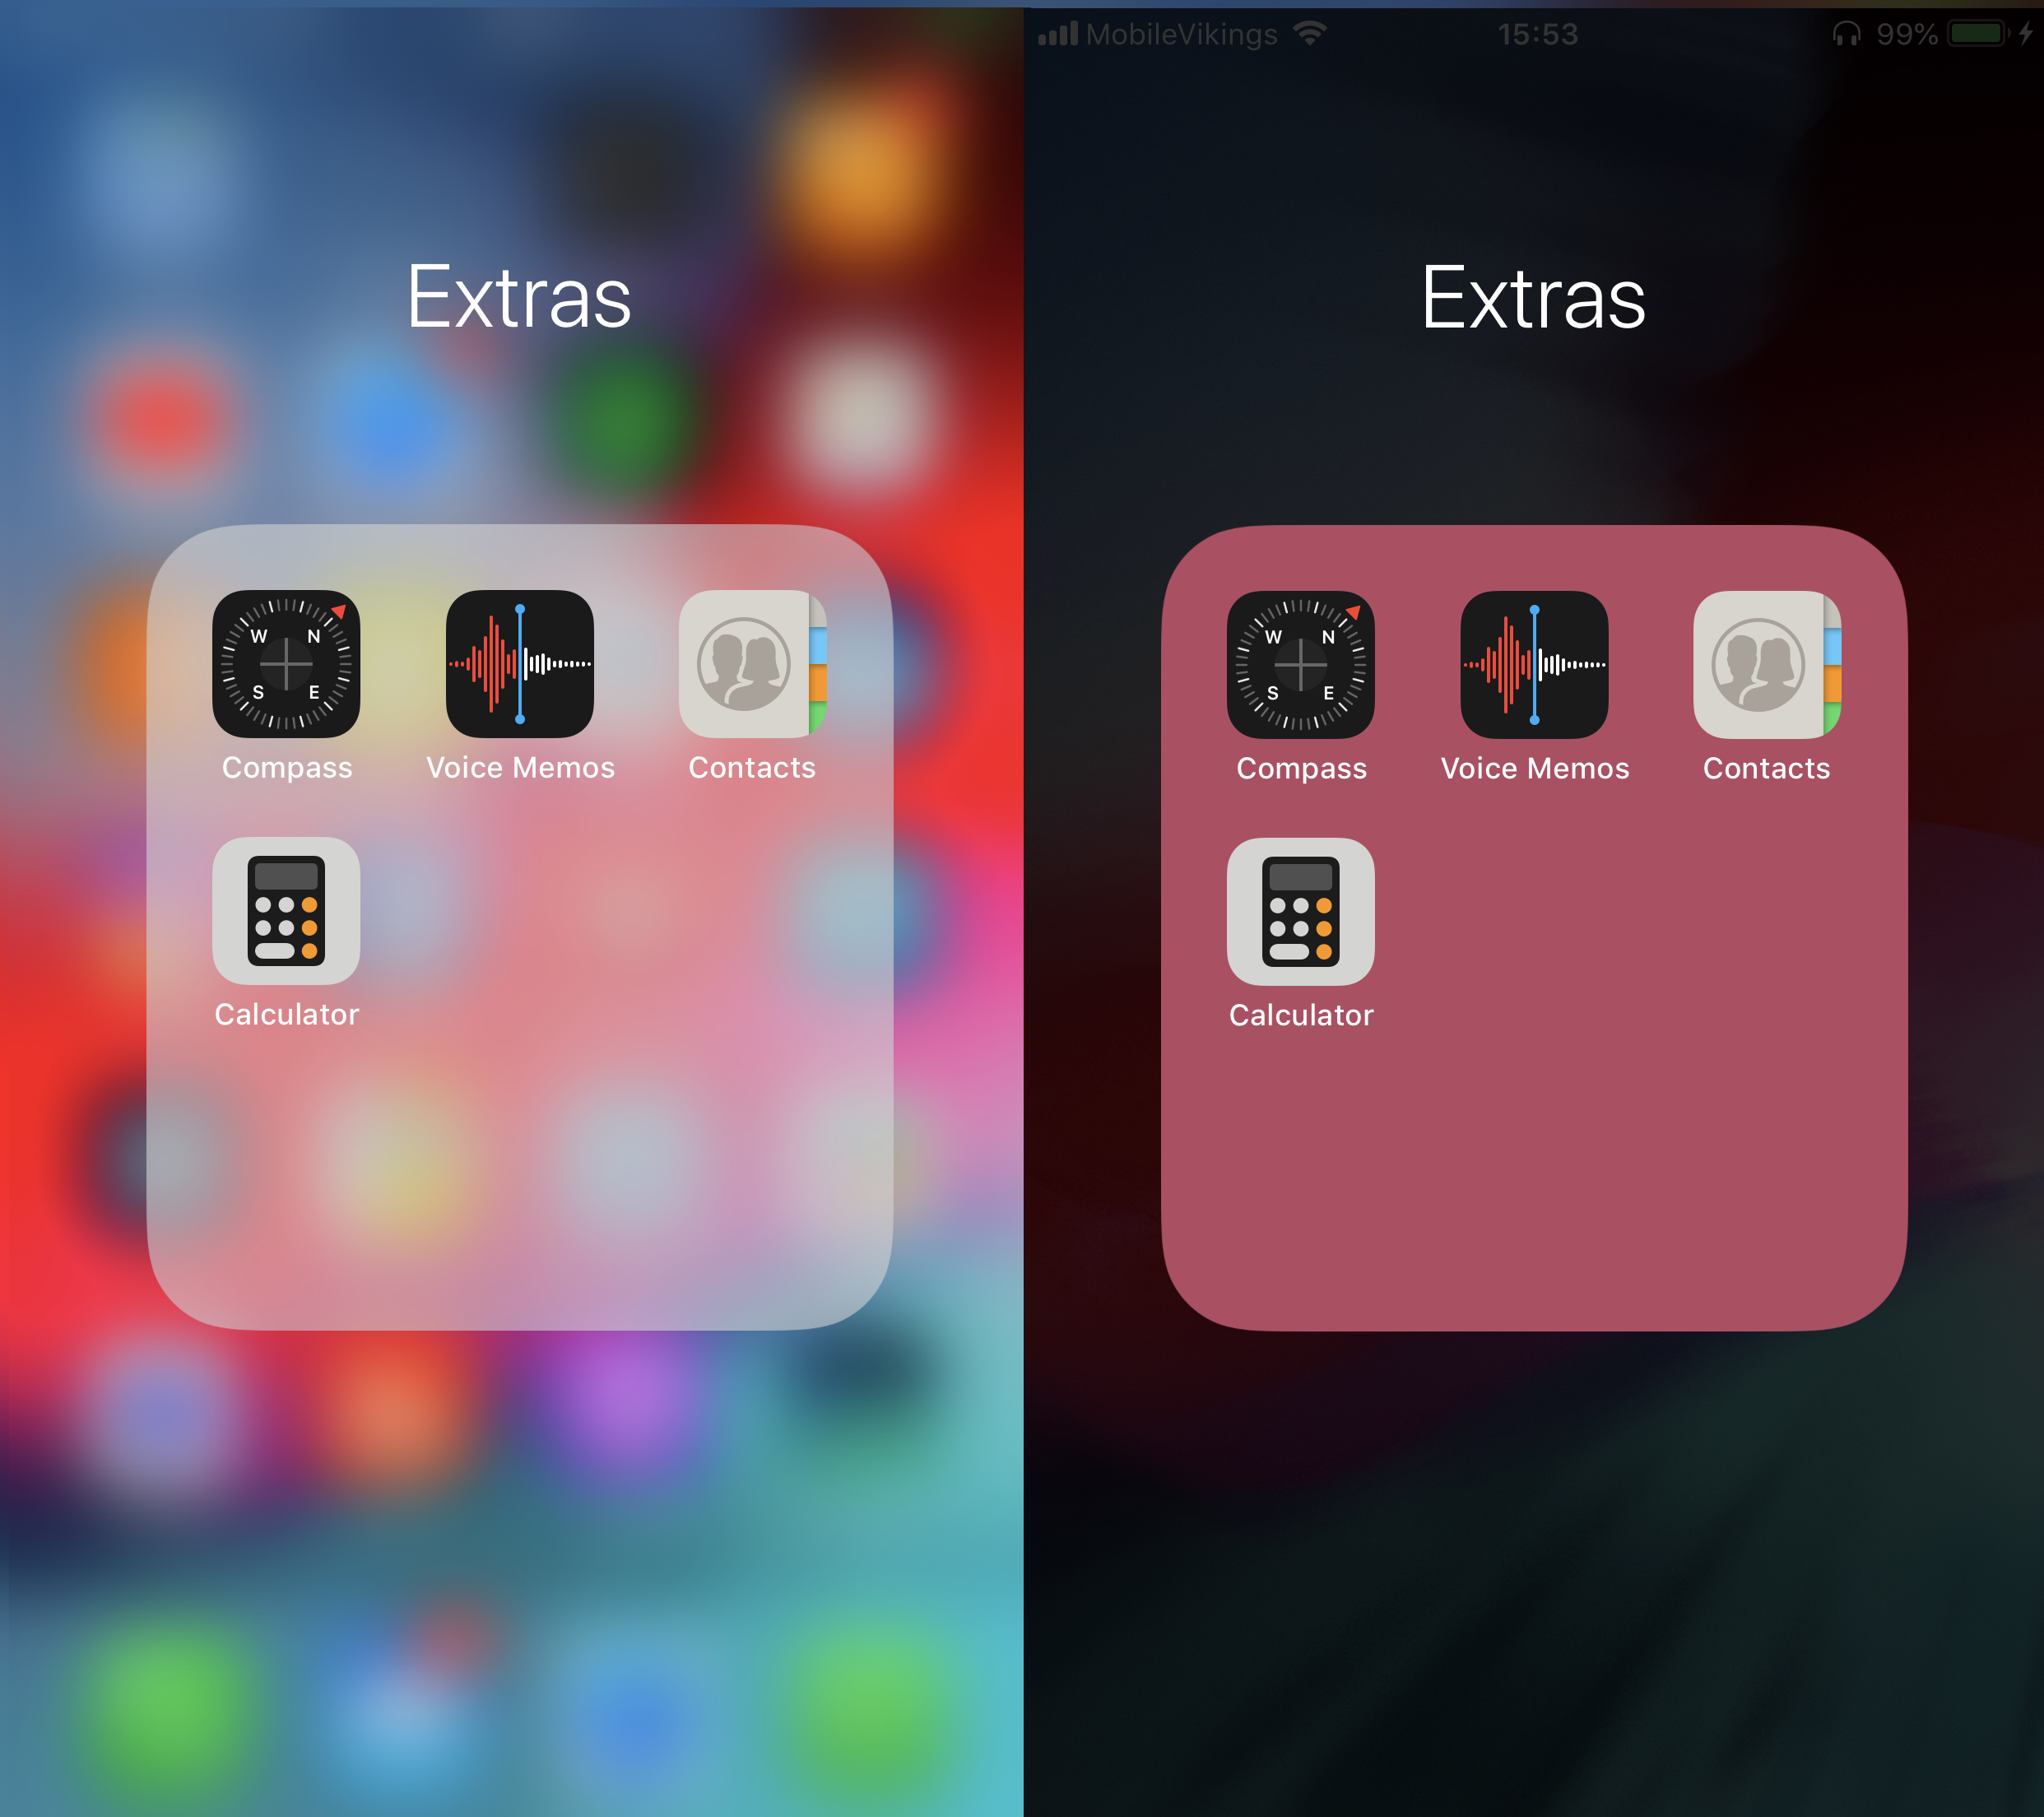
\includegraphics[width=0.7\linewidth]{img/transparantieiOS}}
    \caption{Voorbeeld verminderen transparantie in iOS, links: functionaliteit uit, rechts: functionaliteit aan}
    \label{fig:transparantieiOS}
\end{figure}
\newpage
\subsubsection{Verhogen contrast}
Deze functionaliteit maakt kleuren van elementen donkerder om een hogere contrast te krijgen. Afbeeldingen worden niet aangepast.
Een ontwikkelaar kan via de property \emph{UIAccessibility.isDarkerSystemColorsEnabled} nagaan of deze functionaliteit is ingeschakeld. 
\subsubsection{Vette tekst}
In iOS kan men met de functionaliteit 'Vette tekst' tekst beter leesbaar maken. Alle tekst wordt bij het inschakelen van deze functionaliteit omgezet naar vette tekst.
Via de property \emph{UIAccessibility.isBoldTextEnabled} kan men nagaan of deze functionaliteit is ingeschakeld. 
\subsection{Auditief}
\subsubsection{LED Flash voor notificaties}
Wanneer iemand deze functionaliteit ingeschakeld heeft zal bij een melding zal uit de flits van het toestel een reeks lichtflitsen maken. Deze functionaliteit kan gezien worden als een alternatief voor meldingen met geluid. Men heeft de optie om deze functionaliteit enkel te gebruiken wanneer het geluid van het toestel uit staat.
\subsubsection{Mono-geluid}
Wanneer iemand slechthorend is aan 1 kant kan het wenselijk zijn om beide audio kanalen te combineren naar 1 kanaal. Daardoor kan men alles horen, en mist men geen geluid omdat men maar 1 van de 2 kanalen kon horen. Dankzij deze functionaliteit wordt stereo-geluid aangepast naar mono-geluid.
Via de property \emph{UIAccessibility.isMonoAudioEnabled} kan men nagaan of deze functionaliteit is ingeschakeld.
\subsubsection{Kiezen van balans tussen linker en rechter audiokanaal}
Met deze functionaliteit kan gekozen worden aan de hand van een schuifknop welk audiokanaal men wilt horen. De audiokanalen worden NIET gecombineerd, men zal dus een deel van het afgespeelde geluid verliezen als men de functionaliteit 'Mono-geluid' niet inschakelt. 
\subsubsection{Ondertiteling}
\label{subsec:ondertiteliOS}
Dove of hardhorige mensen gebruiken ondertitelingen als alternatief op audio. Met het inschakelen van deze functionaliteit zullen ondertitelingen weergegeven worden wanneer deze beschikbaar zijn.

Deze functionaliteit is ook nog aanpasbaar naar de voorkeur van de gebruiker. Men kan de stijl van ondertitelingen aanpassen. Er zijn standaard 4 verschillende stijlen, maar die zijn uitbreidbaar met een eigen gemaakte stijl. Wanneer men een nieuwe stijl creëert kan men de tekstkleur, tekstgrootte en lettertype aanpassen. Ook kan de achtergrond en de doorzichtigheid aangepast worden. 

Vaak zullen video's hun vaste stijl gedefinieerd hebben voor ondertiteling, wanneer men een eigen gecreëerde stijl wilt gebruiken zal men  'Video overschrijven' moeten uitschakelen bij alle opties van de eigen gecreëerde stijl.

Een ontwikkelaar kan nagaan of een gebruiker ondertiteling heeft ingeschakeld via de property \emph{UIAccessibility.isClosedCaptioningEnabled}.

Raadpleeg de developer documentatie voor het toevoegen van ondertitelingen aan een AVMediaPlayer\footnote{\url{https://developer.apple.com/streaming/}}.
\subsection{Motorisch}
\subsubsection{Shortcut activatie toegankelijkheidsfunctionaliteiten}
Met deze functionaliteit kunnen personen met een motorische beperking, maar ook met andere beperkingen heel snel hun favoriete functionaliteit activeren. Bij het driemaal indrukken van de homeknop zal de functionaliteit die men geselecteerd heeft geactiveerd worden. Wanneer men meerdere functionaliteiten heeft geselecteerd zal een menu met deze functionaliteiten verschijnen.
\subsubsection{Switch Control}
\label{subsec:schakeliOS}
Switch Control ook wel schakelbediening genoemd laat een gebruiker met een motorische beperking toe om te navigeren binnen iOS. Alle elementen op het scherm worden als het ware één voor één overlopen, waarbij men een element kan activeren door een schakel te gebruiken. Deze schakels kunnen extern zijn, maar kan ook komen vanuit het apparaat. De invoer vanuit het apparaat kunnen knoppen, maar ook touch gebaren zijn. Ook de camera van een apparaat kan gebruikt worden als switch, hierbij kijkt de camera naar bewegingen met het hoofd.

Switch Control is een functionaliteit die zeer aanpasbaar is. Men kan kiezen voor het groeperen van elementen voor snellere navigatie, of voor het afspelen van geluid bij het navigeren, etc.

Een ontwikkelaar kan aan de hand van de property \emph{UIAccessibility.isSwitchControlRunning} weten of iemand Switch Control gebruikt in zijn applicatie. Verder kunnen ontwikkelaars het navigeren in hun applicatie makkelijker maken door elementen te groeperen zoals dit gedaan werd in voorbeeld \ref{dynamicAccessVoiceOverGrouping}.
\subsubsection{AssistiveTouch}
AssistiveTouch maakt het mogelijk om een iOS-apparaat te bedienen zonder de fysieke knoppen te hoeven gebruiken. Bij het activeren van deze functionaliteit krijgt men een menu (AssistiveTouch-menu) op het scherm. Dit menu bevat iconen waarop men kan drukken, elk icoon heeft zijn corresponderende actie in iOS. Zo kan men bijvoorbeeld het scherm vergrendelen, het geluid verhogen, de homeknop bedienen, etc.

Naast het uitvoeren van acties waarvoor men de fysieke knoppen voor zou gebruiken kan men ook touch-gebaren toevoegen als een actie.  Deze gebaren worden dan uitgevoerd wanneer de actie geactiveerd wordt. Deze functionaliteit kan men zeer goed personaliseren, zo kan men kiezen hoeveel acties men in het menu wenst weer te geven. Of men kan 3D Touch gebruiken voor het activeren van een specifieke actie.  Maar ook de doorzichtigheid van het menu kan ingesteld worden.

Als ontwikkelaar kan men nagaan of deze functionaliteit is geactiveerd tijdens het gebruik van zijn applicatie via de volgende propery \emph{UIAccessibility.isAssistiveTouchRunning}.
\subsubsection{Aangepaste aanraking}
\label{subsec:iOSAangepast}
De functionaliteit 'Aangepaste aanraking' is een gecombineerde functionaliteit bestaande uit 3 verschillende functionaliteiten. Ze hebben alle 3 hetzelfde doel, namelijk het aanpassen van hoe het systeem reageert op aanrakingen. Voor onderstaande functionaliteiten te kunnen gebruiken moet men een schakelaar activeren.

De eerste functionaliteit is 'Vasthoudduur' waarbij men kan aanpassen hoelang men het scherm moet indrukken voor iOS het ziet als een aanraking op het touchscreen. Als men een aanraking doet maar men tilt de vinger op voor dat de ingestelde tijd is verstreken zal deze aanraking genegeerd worden. 


Met de functionaliteit 'Negeer herhaling' kan men instellen hoeveel tijd er tussen 2 aanrakingen moet zitten. Hoe langer de tijd die men instelt, hoe langer het besturingssysteem meerdere aanrakingen achter elkaar ziet als 1 aanraking.


De derde functionaliteit 'Tikassistentie' ondersteunt mensen met een motorische beperking die hun vingers ongewenst verplaatsen tijdens het aanraken van het scherm. Zonder deze functionaliteit kan men mogelijk een foutieve selectie maken. Men kan instellen dat iOS bij het aanraken van het scherm ofwel de laatste positie van de aanraking of de eerste positie registreert.

\subsection{Cognitief}
\subsubsection{Verminderen van bewegingen}
Een gebruiker kan met 'Verminderen van bewegingen' ervoor kiezen om animaties te vermijden binnen iOS. Bij het activeren van deze optie worden animaties van het besturingssysteem zelf verwijderd. In tegenstelling tot Android is dit niet het geval bij zelfontwikkelde applicaties.

\lstinputlisting[language=java,label=reduceMotioniOS, caption={Voorbeeld in Swift: Controleren of verminderen van bewegingen is ingeschakeld},frame=single, breaklines,basicstyle=\scriptsize, firstline=18,lastline=30]{../code/iOS/AnimationSample/AnimationSample/ViewController.swift}

Een ontwikkelaar zou bij het gebruik van animaties moeten controleren of een gebruiker deze functionaliteit heeft ingeschakeld. Indien dit het geval is moet de animatie vermeden worden. In voorbeeld \ref{reduceMotioniOS} wordt een animatie uitgevoerd als de optie \emph{UIAccessibility.isReduceMotionEnabled} niet is ingeschakeld.

\subsubsection{Begeleide toegang}
De functionaliteit 'Begeleide toegang' kan wanneer deze geactiveerd is voorkomen dat een gebruiker de applicatie sluit. Dit voorkomt dat een gebruiker afgeleid kan zijn. Enkel bij het ingeven van een wachtwoord, of het aanmelden met FaceID of TouchID kan de applicatie gesloten worden. Naast het voorkomen dat een applicatie gesloten kan worden, kan ook ingesteld worden door een gebruiker in welk gebied geen interactie mogelijk is. Daarnaast kunnen nog diverse zaken ingesteld worden bij het gebruik van een applicatie. Dit kan zijn:
\begin{itemize}
    \item Mogelijkheid tot sluimerknop te gebruiken
    \item Mogelijkheid tot gebruik volumeknoppen
    \item Mogelijkheid tot roteren van scherm
    \item Mogelijkheid tot gebruik toetsenbord
    \item Mogelijkheid tot aanraken van scherm
    \item Tijdslimiet (hoelang de applicatie mag gebruikt worden)
\end{itemize}

Deze functionaliteit kan wanneer deze is ingeschakeld in de instellingen, geactiveerd en gedeactiveerd worden door driemaal kort op de homeknop te drukken. Een ontwikkelaar kan detecteren als de functionaliteit is ingeschakeld in zijn applicatie via de volgende property: \emph{UIAccessibility.isGuidedAccessEnabled}. 

\lstinputlisting[language=java,label=iosAppIdentifierGuided, caption={Voorbeeld in Swift: AppDelegate met applicatie specifieke instellingen voor 'Begeleide toegang'},frame=single, breaklines,basicstyle=\scriptsize, firstline=12,lastline=26]{../code/iOS/GuidedAccess/GuidedAccess/AppDelegate.swift}

Een applicatie kan ook applicatie specifieke instellingen hebben. Deze kunnen bij het activeren van de functionaliteit in de applicatie aan- of uitgezet worden. Met deze instellingen kunnen bepaalde onderdelen van de applicatie geblokkeerd worden, bijvoorbeeld: Toegang tot online wedstrijden in een spelletje.  In voorbeeld \ref{iosAppIdentifierGuided} wordt een applicatie specifieke instelling gedefinieerd. Dit is mogelijk gemaakt door het invullen van de methodes die  overgeërfd werden van het protocol \emph{UIGuidedAccessRestrictionDelegate} in de AppDelegate . De methode \emph{guidedAccessRestrictionIdentifiers} bevat een lijst met alle applicatie specifieke instellingen die men wilt toevoegen. De methode \emph{detailTextForGuidedAccessRestriction(withIdentifier restrictionIdentifier: String)} retourneert voor elke instelling een bijpassende naam. Deze naam is zichtbaar in het instellingen menu.

In voorbeeld \ref{iosAppIdentifierGuidedReaction} wordt een methode gedefinieerd die ook overgeërfd is in de AppDelegate. Deze methode is: \emph{guidedAccessRestriction(withIdentifier restrictionIdentifier: String, didChange newRestrictionState: UIAccessibility.GuidedAccessRestrictionState)}. Met deze methode kan nagegaan worden of een applicatie specifieke instelling geactiveerd werd. Indien dit het geval is kan men dit verder behandelen in de applicatie.
\newpage
\lstinputlisting[language=java,label=iosAppIdentifierGuidedReaction, caption={Voorbeeld in Swift: AppDelegate met methode voor nagaan of applicatie specifieke instelling voor 'Begeleide toegang' werd geactiveerd.'},frame=single, breaklines,basicstyle=\scriptsize, firstline=28,lastline=44]{../code/iOS/GuidedAccess/GuidedAccess/AppDelegate.swift}
%\lipsum[76-80]
\section{Verschillen/gelijkenissen in functionaliteiten Android en iOS}
Uit de bespreking van de toegankelijkheidsfunctionaliteiten in secties \ref{sec:ToegankelijkheidsfunctionaliteitenAndroid} en \ref{sec:ToegankelijkheidsfunctionaliteiteniOS} blijkt,  dat zowel Android als iOS een zeer uitgebreide set aan functionaliteiten bezit. Er kan niet duidelijk gesteld worden dat een besturingssysteem primeert, dit komt vooral door de gelijkenissen en verschillen tussen beide platformen. Wel kan er gesteld worden dat het aantal standaard meegeleverde functionaliteiten kleiner is in Android dan in iOS. In Android is dan weer de mogelijkheid om toegankelijkheidsfunctionaliteiten te downloaden en te ontwikkelen. In de bespreking van de functionaliteiten werden de meest relevante besproken. De virtuele assistenten 'Google Assistant' en 'Siri' werden buiten beschouwing gelaten.


In tabel \ref{overzichtFunctionaliteitenBesproken} vindt u een overzicht met de besproken functionaliteiten. Ook wordt het verschil ten opzichte van functionaliteiten duidelijk gemaakt. Duidelijk zichtbaar is dat de meeste functionaliteiten beschikbaar zijn op beide besturingssystemen. Bij Android werden enkel de standaardfunctionaliteiten besproken. Sommige smartphones met Android kunnen nog extra standaard meegeleverde functionaliteiten bevatten. iOS heeft niet de mogelijkheid om extra functionaliteiten toe te voegen, maar het besturingssysteem bevat wel een brede basis. 

Zowel Android als iOS laten ontwikkelaars toe om toegankelijkheidsfunctionaliteiten te faciliteren in hun applicaties. iOS geeft de ontwikkelaar veel inzicht in welke functionaliteiten ingeschakeld zijn. Wat minder vanzelfsprekend is in Android. Opvallend is dat het schaalbaar maken van tekst veel omslachtiger is in iOS dan in Android. 

\begin{table}
    \centering
    \caption{Overzicht besproken functionaliteiten in Android en iOS per domein}
    \label{overzichtFunctionaliteitenBesproken}
    \begin{tabular}{|l|l|l|} 
        \hline
        \multicolumn{3}{|l|}{\textbf{Visueel} }                                                        \\ 
        \hline
        \textbf{Beschrijving}                                 & \textbf{Android}  & \textbf{iOS}       \\ 
        \hline
        Navigeren via audio feedback                          & TalkBack          & VoiceOver          \\ 
        \hline
        Schalen van lettertypes                               & Ja                & Ja                 \\ 
        \hline
        Schalen van weergave grootte~                         & Ja                & Nee                \\ 
        \hline
        Inzoomen op elementen                                 & Ja                & Ja                 \\ 
        \hline
        Filters voor kleurenblindheid                         & Ja                & Ja                 \\ 
        \hline
        Verhogen contrast~                                    & Ja                & Ja                 \\ 
        \hline
        Inverteren kleuren                                    & Ja                & Ja                 \\ 
        \hline
        Vette tekst                                           & Nee~              & Ja                 \\ 
        \hline
        \multicolumn{3}{|l|}{}                                                                         \\ 
        \hline
        \multicolumn{3}{|l|}{\textbf{Auditief}}                                                        \\ 
        \hline
        \textbf{Beschrijving}                                 & \textbf{Android~} & \textbf{iOS}       \\ 
        \hline
        Mono-geluid                                           & Ja                & Ja                 \\ 
        \hline
        (Aanpasbare) ondertiteling                            & Ja                & Ja                 \\ 
        \hline
        Geluidsversterker                                     & Ja                & Beperkt            \\ 
        \hline
        LED flash voor notificaties                           & Nee               & Ja                 \\ 
        \hline
        \multicolumn{3}{|l|}{}                                                                         \\ 
        \hline
        \multicolumn{3}{|l|}{\textbf{Motorisch}}                                                       \\ 
        \hline
        \textbf{Beschrijving}                                 & \textbf{Android}  & \textbf{iOS}       \\ 
        \hline
        Hardware knoppen voor besturen                        & Ja                & Ja                 \\ 
        \hline
        Scherm automatisch draaien                            & Ja                & Ja                 \\ 
        \hline
        Vertragingen bij aanraken                             & Ja                & Ja                 \\ 
        \hline
        Hardware activatie van functionaliteiten              & Ja                & Ja                 \\ 
        \hline
        Vervanging van hardware knoppen                       & Nee               & AssistiveTouch     \\ 
        \hline
        \multicolumn{3}{|l|}{}                                                                         \\ 
        \hline
        \multicolumn{3}{|l|}{\textbf{Cognitief}}                                                       \\ 
        \hline
        \textbf{Beschrijving}                                 & \textbf{Android}  & \textbf{iOS}       \\ 
        \hline
        Verwijderen van animaties                             & Ja                & Ja                 \\ 
        \hline
        Beperken van afleiding bij gebruik van een applicatie & Nee               & Begeleide toegang  \\
        \hline
    \end{tabular}
\end{table}
\chapter{\IfLanguageName{dutch}{Richtlijnen voor mobiele applicaties}{Richtlijnen voor  mobiele applicaties}}
\label{ch:Richtlijnen voor toegankelijkheid mobiele applicaties}
Een ontwikkelaar moet kunnen nagaan of zijn mobiele applicatie toegankelijk is. De bestaande richtlijnen zijn intimiderend, en moeilijk toepasbaar op mobiele applicaties. Daardoor kan men moeilijk toetsen wanneer men een toegankelijke mobiele applicatie heeft. In dit hoofdstuk wordt aan de hand van de WCAG richtlijnen een maatstaf opgesteld voor ontwikkelaars. Hierdoor kan vlot een inzicht gecreëerd worden over de toegankelijkheid van een mobiele applicatie.

\section{WCAG richtlijnen}
\label{sec:WCAGrichtlijn}

Zoals reeds besproken is in sectie \ref{sec:wetgeving} vormen de WCAG richtlijnen de basis voor dit onderzoek. Meer bepaald de richtlijnen die besproken zijn in WCAG 2.1. Deze richtlijnen bevatten extra criteria gericht op het gebruik van touchscreens, visuele beperkingen en cognitieve beperkingen.
De succescriteria beschreven in de WCAG richtlijnen zijn technologie onafhankelijk opgesteld. Dit wil zeggen dat ze zowel op mobiele platformen als computers kunnen toegepast worden\autocite{w3cTechnologyNeutral}. Vaak wordt het woord 'web' gebruikt in een richtlijn, wat in de meeste gevallen vervangen kan worden door 'mobiele applicatie'. Bij sommige richtlijnen is verdere interpretatie vereist. Dit onderzoek zal dan ook proberen de bestaande richtlijnen te vertalen naar richtlijnen voor mobiele applicaties.

De WCAG 2.1 richtlijnen zijn opgebouwd in een specifieke structuur. De richtlijnen en de daarbij horende succescriteria zijn onderverdeeld onder vier verschillende principes. Aan deze principes moet voldaan worden om een toegankelijke applicatie te hebben. Deze principes zijn respectievelijk: 
\begin{itemize}
    \item Waarneembaar: gebruikers moeten de informatie (op het scherm) kunnen waarnemen.
        \item Bedienbaar: gebruikers moeten kunnen de elementen kunnen bedienen, waaronder ook navigatie.
        \item Begrijpelijk: gebruikers moeten de informatie en bediening van een applicatie verstaan.
        \item Robuust: gebruikers moeten de inhoud blijven kunnen gebruiker wanneer ze nieuwe technologie gebruiken.
\end{itemize}

Binnen de principes zijn er richtlijnen. Deze richtlijnen bevatten de doelen die men moet behalen voor aan een principe te voldoen. Die doelen kunnen behaald worden door de applicatie te toetsen aan succescriteria. Een succescriteria schrijft vereisten voor waaraan voldaan moet worden om een richtlijn te kunnen behalen. 

Elk succescriteria bevat een niveau, deze niveaus komen overeen met de afstemming op de behoeften van gebruikers met een beperking. Deze levels zijn:
\begin{itemize}
    \item Niveau A: Minimum level, voldoet aan niveau A succescriteria.
    \item Niveau AA: Voldoet aan niveau A succescriteria en niveau AA succescriteria.
    \item Niveau AAA: Voldoet aan niveau A, AA en AAA succescriteria.
\end{itemize}

Binnen dit onderzoek zullen wij ons focussen op niveau A en niveau AA succesfactoren. De WCAG richtlijnen raden af om alle succescriteria te proberen afstemmen tot niveau AAA. Ze vermelden dat het onmogelijk is om deze allemaal te behalen. 

Als voorbeeld:  \emph{Succesfactor 1.2.6: Er wordt een gebarentaalvertolking geleverd voor alle vooraf opgenomen audiocontent in gesyncroniseerde media. (Level AAA)}. Er kan gesteld worden, dat dit onmogelijk is voor vele applicaties om daaraan te voldoen \autocite{WCAG2.1Criteria}.

In het vervolg van deze sectie gaan wordt per principe de richtlijnen en succesfactoren bespreken. Om een indruk te kunnen geven van de potentiële impact op de gebruikers van een succesfactor wordt er een score aan toegekend. Deze score drukt de potentiële impact uit op de gebruikservaring van de app (of een specifieke functionaliteit ervan) voor een van de 4 (ruim gedefinieerde) doelgroepen.
Hoe hoger de score, hoe aannemelijker het is dat een correcte toepassing van dit WCAG-criterium een bovengemiddelde impact heeft op de gebruikerservaring. De scores hebben de volgende betekenis:
\begin{enumerate}
    \item Geen bovengemiddelde impact
    \item Bovengemiddelde impact
    \item Essentiële impact
\end{enumerate}


\newpage
\section{WCAG-richtlijnen voor mobiele applicaties}
\label{sec:WCAGrichtlijnMobiel}
De onderstaande principes, richtlijnen en succesfactoren zijn dus gebaseerd op de bestaande WCAG 2.1 richtlijnen\footnote{\url{https://www.w3.org/WAI/WCAG21/quickref/}}. Deze worden vertaalt naar het gebruik in mobiele applicaties. De succesfactoren die moeilijk toepasbaar op mobiele applicaties zijn, of teveel focussen op inhoud, worden buiten beschouwing gelaten. Dit onderzoek richt zich enkel op welke inspanningen een ontwikkelaar kan doen voor het toegankelijk maken van een mobiele applicatie. Voor te voldoen aan de WCAG 2.1 niveau AA richtlijnen, dienen de succesfactoren die focussen op inhoud ook in acht genomen te worden.
\subsection{Principe 1: Waarneembaar}
\label{sec:waarneembaarWCAG}
Dit principe stelt dat informatie en elementen van een applicatie gepresenteerd moeten worden zodanig dat men die kan waarnemen.


\subsubsection{Richtlijn 1.1 - Tekst alternatieven}
Gebruikers kunnen nood hebben aan een alternatief voor inhoud die geen tekst bevat. Voor deze richtlijn te faciliteren moet aan de succesfactoren in tabel xx voldaan worden.
\newpage
\begin{table}[H]
    \centering
    \caption{Succesfactor 1.1.1: niet-tekst inhoud}
 \hspace*{-1cm}\begin{tabular}{|l|p{12cm}|} 
        \hline
        \textbf{Succesfactor}                & 1.1.1                                                                                                                                                                                                                                                                                                             \\ 
        \hline
        \textbf{Level}                       & A                                                                                                                                                                                                                                                                                                                                                                             \\ 
        \hline
        \textbf{Naam}                        & Niet-tekst inhoud~                                                                                                                                                                                                                                                                                                                                                            \\ 
        \hline
        \textbf{Slagen van succesfactor}     & \begin{itemize}
            \item Tekstalternatieven voorzien voor niet-tekst inhoud (bv. afbeeldingen, knoppen, …)
        \end{itemize}                                                                                                                                                                                                      \\ 
        \hline
        \textbf{Beschrijving}                & Vooral gebruikers met een visuele beperking zullen gebruik maken van VoiceOver of TalkBack. Ze besturen hun smartphone via audio feedback. Alle elementen die tekst bevatten worden voorgelezen. Sommige elementen bevatten geen of weinig betekenisvolle tekst. Men moet dus goede tekst alternatieven voorzien voor niet-tekst inhoud.  \\ 
        \hline
        \textbf{Impact op gebruikers}        & 
        \begin{itemize}
            \item Visueel: 3, verhoogt het waarnemen van inhoud.
            \item Cognitief: 2, maakt makkelijker om inhoud op te nemen.             
        \end{itemize}                                                                                                                   \\ 
        \hline
        \textbf{Platform specifieke feature} & \begin{itemize}
            \item iOS: VoiceOver, zie \ref{subsec:VoiceOver}.
            \item Android: TalkBack, zie \ref{subsec:TalkBack}
        \end{itemize}                                                                                                                                                                       \\ 
        \hline
        \textbf{Testen}                      & Deze succesfactor kan getest worden door een ontwikkelaar met ofwel TalkBack of VoiceOver de mobiele applicatie te besturen. Wanneer een element niet duidelijk benoemd is (voornamelijk afbeeldingen), kan gesteld worden dat er niet voldaan wordt aan het succescriteria.                                                                                                                                                                                                                        \\
        \hline
    \end{tabular}
\end{table}



\subsubsection{Richtlijn 1.2: Tijds-gebaseerde media}
Gebruikers moeten een alternatief hebben voor tijds-gebaseerde media. Dit is zowel vooraf opgenomen media als live media. De volgende succesfactoren worden gebruikt: \begin{itemize}
    \item Succesfactor 1.2.1: vooraf opgenomen geluid of beeld (A)
    \item Succesfactor 1.2.2: ondertitelingen bij vooraf opgenomen video’s met audio (A)
    \item Succesfactor 1.2.3: audiodescriptie of alternatief bij vooraf opgenomen video’s met audio (A)
    \item Succesfactor 1.2.4: ondertitelingen bij live video’s met audio (AA)
    \item Succesfactor 1.2.5: audiodescriptie bij vooraf opgenomen video’s met audio (AA)
\end{itemize}
\begin{table}[H]
    \centering
    \caption{Succesfactor 1.2.1: vooraf opgenomen geluid of beeld}
    \hspace*{-1cm}\begin{tabular}{|l|p{12cm}|} 
        \hline
        \textbf{Succesfactor}                & 1.2.1                                                                                                                                                                                                                                                                                                             \\ 
        \hline
        \textbf{Level}                       & A                                                                                                                                                                                                                                                                                                                                                                             \\ 
        \hline
        \textbf{Naam}                        & Vooraf opgenomen geluid of beeld~                                                                                                                                                                                                                                                                                                                                                            \\ 
        \hline
        \textbf{Slagen van succesfactor}     & \begin{itemize}
            \item Bij enkel audio: een tekst transcript voorzien.
            \item Bij enkel video: een audio fragment of tekst transcript voorzien.
        \end{itemize}                                                                                                                                                                                                      \\ 
     \hline
    \textbf{Uitzondering}     & 
        Wanneer de media een alternatief is voor tekst (die aanwezig is), hoeft er geen rekening gehouden te worden voor dat media element.                                                                                                                                                                                                     \\ 
        \hline
        \textbf{Beschrijving}                & Wanneer men te maken heeft met inhoud die ofwel geluid of beeld moet een alternatief voorzien worden. Bij bijvoorbeeld een audio is een transcriptie die beschrijft wat er gebeurt gewenst. Bij video is een transcriptie of een audio track die beschrijft wat er te horen valt gewenst. \\ 
        \hline
        \textbf{Impact op gebruikers}        & 
        \begin{itemize}
            \item Visueel: 3, verhoogt het waarnemen van inhoud (bij beeld).
            \item Auditief 3, verhoogt waarnemen van inhoud (bij geluid).             
        \end{itemize}                                                                                                                   \\ 
        \hline
        \textbf{Testen}                      & Men kan nagaan of voldaan wordt aan de richtlijn, wanneer men er niet in slaagt, kan gesteld worden dat men niet voldoet aan de richtlijn.                                                                                                                                                                                                            \\
        \hline
    \end{tabular}
\end{table}
\newpage
\begin{table}[H]
    \centering
        \caption{Succesfactor 1.2.2: ondertitelingen bij vooraf opgenomen video’s met audio}
    \hspace*{-1cm}\begin{tabular}{|l|p{12cm}|} 
        \hline
        \textbf{Succesfactor}                & 1.2.2                                                                                                                                                                                                                                                                                                             \\ 
        \hline
        \textbf{Level}                       & A                                                                                                                                                                                                                                                                                                                                                                             \\ 
        \hline
        \textbf{Naam}                        & Ondertitelingen bij vooraf opgenomen video’s met audio~                                                                                                                                                                                                                                                                                                                                                            \\ 
        \hline
        \textbf{Slagen van succesfactor}     & \begin{itemize}
            \item Ondertitelingen toevoegen aan video’s waar geluid is.
        \end{itemize}                                                                                                                                                                                                      \\ 
        \hline
        \textbf{Uitzondering}     & Wanneer de video een alternatief is voor tekst (die aanwezig is), hoeft er geen rekening gehouden te worden met de succesfactor.
                                                                                                                                                                                                      \\ 
        \hline
        \textbf{Beschrijving}                & Ondertitelingen worden vaak gebruikt bij gebruikers met een auditieve beperking. Het biedt een tekstalternatief voor de audio die afgespeeld wordt in een video. \\ 
        \hline
        \textbf{Impact op gebruikers}        & 
        \begin{itemize}
            \item Auditief 3, verhoogt waarnemen van inhoud.             
        \end{itemize}                                                                                                                   \\ 
      \hline
    \textbf{Platform specifieke feature} & \begin{itemize}
        \item iOS: zie \ref{subsec:ondertiteliOS}.
        \item Android: zie \ref{subsec:ondertitelAndroid}
    \end{itemize}                                                                                                                                                                       \\ 
        \hline
        \textbf{Testen}                      & Men kan nagaan of voldaan wordt aan de richtlijn. Wanneer een video, die niet dient als alternatief voor een tekst, geen ondertitelingen ondersteunt, kan gesteld worden dat er niet voldaan wordt.                                                                                                                                                                                              \\
        \hline
    \end{tabular}
\end{table}

\begin{table}[H]
    \centering
       \caption{Succesfactor 1.2.3: audiodescriptie of alternatief bij vooraf opgenomen video’s met audio}
    \hspace*{-1cm}\begin{tabular}{|l|p{12cm}|} 
        \hline
        \textbf{Succesfactor}                & 1.2.3                                                                                                                                                                                                                                                                                                             \\ 
        \hline
        \textbf{Level}                       & A                                                                                                                                                                                                                                                                                                                                                                             \\ 
        \hline
        \textbf{Naam}                        & Audiodescriptie of alternatief bij vooraf opgenomen video’s met audio~                                                                                                                                                                                                                                                                                                                                                            \\ 
        \hline
        \textbf{Slagen van succesfactor}     & \begin{itemize}
            \item Een audio beschrijving te voorzien voor video’s, of
            \item een volledig transcript van de video voorzien.
        \end{itemize}                                                                                                                                                                                                      \\ 
        \hline
        \textbf{Uitzondering}     &  Wanneer de video een alternatief is voor tekst (die aanwezig is), hoeft er geen rekening gehouden te worden met de succesfactor.
                                                                                                                                                                                                         \\ 
        \hline
        \textbf{Beschrijving}                & Gebruikers met een visuele een beperking wensen graag een beschrijving van wat er gebeurt in een video. Een audiodescriptie geeft deze gebruikers via geluid uitleg wat er te zien valt in de video. Dit kan gebeuren via een audio descriptie, of een transcript te voorzien. Dit transcript kan door de screenreader dan voorgelezen worden.\\ 
        \hline
        \textbf{Impact op gebruikers}        & 
        \begin{itemize}
            \item Visueel 3, verhoogt waarnemen van inhoud.    
            \item Cognitief 2, verhoogt verstaanbaarheid bewegende beelden         
        \end{itemize}                                                                                                                   \\ 
      
        \hline
        \textbf{Testen}                      & Men kan nagaan of voldaan wordt aan de richtlijn. Wanneer een video, die niet dient als alternatief voor een tekst, een audio beschrijving heeft, of een transcript van de audio voorzien is. Dan slaagt men met het implementeren van deze succesfactor.                                                                                                                               \\
        \hline
    \end{tabular}
\end{table}

\begin{table}[H]
    \centering
       \caption{Succesfactor 1.2.4: ondertitelingen bij live video’s met audio}
    \hspace*{-1cm}\begin{tabular}{|l|p{12cm}|} 
        \hline
        \textbf{Succesfactor}                & 1.2.4                                                                                                                                                                                                                                                                                                             \\ 
        \hline
        \textbf{Level}                       & AA                                                                                                                                                                                                                                                                                                                                                                             \\ 
        \hline
        \textbf{Naam}                        & Ondertitelingen bij live video’s met audio~                                                                                                                                                                                                                                                                                                                                                            \\ 
        \hline
        \textbf{Slagen van succesfactor}     & \begin{itemize}
            \item Ondertitelingen toevoegen aan live video’s waar geluid is.
        \end{itemize}                                                                                                                                                                                                      \\ 
        \hline
        \textbf{Beschrijving}                & Gebruikers met een auditieve beperking hebben vooral baat bij het gebruik van ondertite- lingen in een live video met geluid.  \\ 
        \hline
        \textbf{Impact op gebruikers}        & 
        \begin{itemize}
            \item Auditief 3, verhoogt waarnemen van inhoud.             
        \end{itemize}                                                                                                                   \\ 
        \hline
        \textbf{Platform specifieke feature} & \begin{itemize}
            \item iOS: zie \ref{subsec:ondertiteliOS}.
            \item Android: zie \ref{subsec:ondertitelAndroid}
        \end{itemize}                                                                                                                                                                       \\ 
        \hline
        \textbf{Testen}                      & Elke live video met geluid moet ondertitelingen bevatten bij het activeren ervan.                                                                                                                                                                                    \\
        \hline
    \end{tabular}
\end{table}


\begin{table}[H]
    \centering
    \caption{Succesfactor 1.2.5: audiodescriptie bij vooraf opgenomen video’s met audio}
    \hspace*{-1cm}\begin{tabular}{|l|p{12cm}|} 
        \hline
        \textbf{Succesfactor}                & 1.2.5                                                                                                                                                                                                                                                                                                             \\ 
        \hline
        \textbf{Level}                       & AA                                                                                                                                                                                                                                                                                                                                                                             \\ 
        \hline
        \textbf{Naam}                        & Audiodescriptie bij vooraf opgenomen video’s met audio~                                                                                                                                                                                                                                                                                                                                                            \\ 
        \hline
        \textbf{Slagen van succesfactor}     & \begin{itemize}
            \item Een audio beschrijving te voorzien voor video’s.
        \end{itemize}                                                                                                                                                                                                                         \\ 
    \hline
\textbf{Uitzondering}     &
 Wanneer de video een alternatief is voor tekst (die aanwezig is), hoeft er geen rekening gehouden te worden met de succesfactor.                                                                                                                                                                                                                                                                                  \\ 
        \hline
        \textbf{Beschrijving}                & Deze succesfactor leunt sterk aan tegen succesfactor 1.2.3. Deze overlapping komt doordat men in 1.2.5 (niveau AA) iets hogere vereisten stelt. In 1.2.3 heeft men de keuze voor een transcript, of een audiodescriptie te voorzien. In 1.2.5 wordt men verplicht om een audiodescriptie te voorzien. \\ 
        \hline
        \textbf{Impact op gebruikers}        & 
        \begin{itemize}
            \item Visueel 3, verhoogt waarnemen van inhoud. 
            \item Cognitief 2, laat toe bewegende beelden beter te verstaan            
        \end{itemize}                                                                                                                   \\ 
       
        \hline
        \textbf{Testen}                      & Men kan nagaan of voldaan wordt aan de richtlijn. Wanneer een video, die niet dient als alternatief voor een tekst, een audio beschrijving heeft. Dan slaagt men met het implementeren van deze succesfactor.                                                                                                                                                              \\
        \hline
    \end{tabular}
\end{table}

%\paragraph{Succesfactor 1.2.5: Audiodescriptie bij vooraf opgenomen video's met audio (AA)}
%Deze succesfactor leunt sterk aan tegen succesfactor 1.2.3. Deze overlapping komt doordat men in 1.2.5 (niveau AA) iets hogere vereisten stelt. 
%In 1.2.3 heeft men de keuze voor een transcript, of een audiodescriptie te voorzien. In 1.2.5 wordt men verplicht om een audiodescriptie te voorzien. 

%Om te voldoen aan deze succesfactor dient men: 
%\begin{itemize}
%   \item Een audio beschrijving te voorzien voor video's.
    
%\end{itemize}
%Men hoeft geen rekening te houden met deze succesfactor wanneer de video een alternatief is voor een tekst.

%Een succesvolle implementatie van de succesfactor biedt voordeel aan:
%\begin{itemize}
  %  \item Visuele beperking: moeilijkheden waarnemen van beeld.
  %  \item Cognitieve beperking: moeilijkheden verstaan van bewegende beelden.
%\end{itemize}


\subsubsection{Richtlijn 1.3 - Aanpasbaar}
Deze richtlijn focust op het feit dat alle informatie beschikbaar is in de vorm waarin hij kan waargenomen worden. Bijvoorbeeld door het gebruik van VoiceOver of TalkBack. Daarvoor moet de informatie in een applicatie kunnen waargenomen worden door die software. Binnen deze richtlijn worden de volgende succesfactoren gebruikt: \begin{itemize}
    \item Succesfactor 1.3.1: informatie en relaties tussen informatie (A)
    \item Succesfactor 1.3.2: betekenisvolle volgorde (A)
        \item Succesfactor 1.3.3: zintuiglijke eigenschappen (A)
              \item Succesfactor 1.3.4: oriëntatie scherm (AA)
              \item Succesfactor 1.3.5: identificeerbaar doel van invoerveld (AA)
\end{itemize}

\newpage
\begin{table}[H]
    \centering
    \caption{Succesfactor 1.3.1: informatie en relaties tussen informatie}
    \hspace*{-1cm}\begin{tabular}{|l|p{12cm}|} 
        \hline
        \textbf{Succesfactor}                & 1.3.1                                                                                                                                                                                                                                                                                                             \\ 
        \hline
        \textbf{Level}                       & A                                                                                                                                                                                                                                                                                                                                                                             \\ 
        \hline
        \textbf{Naam}                        & Informatie en relaties tussen informatie~                                                                                                                                                                                                                                                                                                                                                            \\ 
        \hline
        \textbf{Slagen van succesfactor}     & \begin{itemize}
            \item Alle informatie dient waarneembaar te zijn door een screenreader.
        \end{itemize}                                                                                                                                                                                                                       
        \\ 
        \hline
        \textbf{Beschrijving}                & Een gebruiker die gebruik maakt van een screenreader voor te navigeren. Alle informatie op het scherm moet daarvoor kunnen bepaald worden door die software. \\ 
        \hline
        \textbf{Impact op gebruikers}        & 
        \begin{itemize}
            \item Visueel 3, verhoogt waarnemen van inhoud.         
        \end{itemize}                                                                                                                   \\ 
        \hline
        \textbf{Platform specifieke feature} & \begin{itemize}
            \item iOS: zie \ref{subsec:ondertiteliOS}.
            \item Android: zie \ref{subsec:ondertitelAndroid}
        \end{itemize}                                                                                                                                                                       \\ 
        
        \hline
        \textbf{Testen}                      & Men kan nagaan of voldaan wordt aan de richtlijn. Wanneer alle informatie die op het scherm weergegeven is, waarneembaar is door een screenreader voldoet men aan deze succesfactor.                                                                                                                                                        \\
        \hline
    \end{tabular}
\end{table}

\begin{table}[H]
    \centering
    \caption{Succesfactor 1.3.2: betekenisvolle volgorde}
    \hspace*{-1cm}\begin{tabular}{|l|p{12cm}|} 
        \hline
        \textbf{Succesfactor}                & 1.3.2                                                                                                                                                                                                                                                                                                            \\ 
        \hline
        \textbf{Level}                       & A                                                                                                                                                                                                                                                                                                                                                                             \\ 
        \hline
        \textbf{Naam}                        & Betekenisvolle volgorde~                                                                                                                                                                                                                                                                                                                                                            \\ 
        \hline
        \textbf{Slagen van succesfactor}     & \begin{itemize}
            \item De inhoud van een mobiele applicatie moet logisch geordend zijn.
            \item Gerelateerde informatie dient gegroepeerd te worden.
        \end{itemize}                                                                                                                                                                                                                         
        \\ 
        \hline
        \textbf{Beschrijving}                & Bij het gebruik van een screenreader kan volgorde van de informatie vaak van belang zijn. Een gebruiker met een visuele beperking, voornamelijk blinden zullen moeite hebben met de context van de informatie. Wanneer deze niet logisch gerangschikt, gegroepeerd staat,
        kan dit problemen geven. \\ 
        \hline
        \textbf{Impact op gebruikers}        & 
        \begin{itemize}
            \item Visueel 3, verhoogt waarnemen van inhoud op een correcte wijze.         
        \end{itemize}                                                                                                                   \\ 
        \hline
        \textbf{Platform specifieke feature} & \begin{itemize}
            \item iOS: zie \ref{subsec:ondertiteliOS}.
            \item Android: zie \ref{subsec:ondertitelAndroid}
        \end{itemize}                                                                                                                                                                       \\ 
        
        \hline
        \textbf{Testen}                      & Men kan nagaan of voldaan wordt aan de richtlijn. Informatie die aan elkaar verbonden is moet achter elkaar uitgesproken worden.  Voorbeeld: wanneer men 2 elementen heeft (labels), met de tekst 'Totale balans' en '50 euro', is het zinvol dat die vlak na elkaar uitgesproken worden.                                                                                                                                                     \\
        \hline
    \end{tabular}
\end{table}

\begin{table}
    \centering
    \caption{Succesfactor 1.3.3: zintuiglijke eigenschappen }
     \hspace*{-1cm}\begin{tabular}{|l|p{12cm}|} 
        \hline
        \textbf{Succesfactor}                 & 1.3.3                                                                                                                                                                                                                                                                                                                                                                                                                                                                                                             \\ 
        \hline
        \textbf{Level}                        & A                                                                                                                                                                                                                                                                                                                                                                                                                                                                                                                 \\ 
        \hline
        \textbf{Naam}                         & Zintuiglijke eigenschappen~~                                                                                                                                                                                                                                                                                                                                                                                                                                                                                      \\ 
        \hline
        \textbf{Slagen van succesfactor}      & Instructies geven die waarneembaar zijn voor verschillende zintuigen (visueel, auditief, ...).                                                                                                                                                                                                                                                                                                                                                                                                                    \\ 
        \hline
        \textbf{Beschrijving}                 & Deze succesfactor verhindert dat gebruikers met een visuele beperking een mobiele applicatie niet kunnen bedienen door onduidelijke instructies. Bijvoorbeeld: een blinde gebruiker zal niks zijn met de instructie om op de derde knop links te drukken. Voor zo’n actie uit te voeren mag men niet blind zijn. Hetzelfde voor mensen met een auditieve beperking, wanneer instructies enkel via geluid worden gegeven, kan deze gebruiker geen actie ondernemen.  \\ 
        \hline
        \textbf{Impact op gebruikers}         &  
        \begin{itemize}
            \item Visueel 3
            \item Auditief 3   
        \end{itemize}                                                                                                                                                                                                                                                                                                                                                                                                                    \\ 
        \hline
        \textbf{Platform specifieke feature}  & Men kan in iOS eventueel inspelen als developer op de properties in de klasse~\textit{UIAccessibility}. In Android kan men van bepaalde instellingen de waarden opvragen.                                                                                                                                                                                                                                                                                                                                         \\ 
        \hline
        \textbf{Testen}                       & Men kan nagaan of voldaan wordt aan de richtlijn. Wanneer instructies niet waarneembaar zijn voor meer dan 1 zintuig, dan slaagt men niet in het voldoen aan deze succesfactor                                                                                                                                                                                                                                                                                                                                    \\
        \hline
    \end{tabular}
\end{table}




%\paragraph{Succesfactor 1.3.1:  Informatie en relaties tussen informatie (A)}
%Een gebruiker die gebruik maakt van een screenreader voor te navigeren. Alle informatie op het scherm moet daarvoor kunnen bepaald worden door die software. Voor deze succesfactor te implementeren dient:
%\begin{itemize}
%    \item Alle informatie waarneembaar te zijn door een screenreader.
%\end{itemize}
%Een succesvolle implementatie van de succesfactor biedt voordeel aan:
%\begin{itemize}
%    \item Visuele beperking: elementen op scherm worden correct voorgelezen.
%\end{itemize}
%Zie sectie \ref{subsec:TalkBack} en \ref{subsec:VoiceOver} voor details over de implementatie.

%\paragraph{Succesfactor 1.3.2:  Betekenisvolle volgorde (A)}
%Bij het gebruik van een screenreader kan volgorde van de informatie vaak van belang zijn. Een gebruiker met een visuele beperking, voornamelijk blinden zullen moeite hebben met de context van de informatie. Wanneer deze niet logisch gerangschikt, gegroepeerd staat, kan dit problemen geven.
%Om deze succesfactor succesvol te implementeren dient:
%\begin{itemize}
%    \item De inhoud logisch geordend zijn.
 %   \item Gerelateerde informatie gegroepeerd staan.
%\end{itemize}
%Een succesvolle implementatie van de succesfactor biedt voordeel aan:
%\begin{itemize}
%    \item Visuele beperking: elementen op scherm worden correct voorgelezen.
%\end{itemize}
%Zie sectie \ref{subsec:TalkBack} en \ref{subsec:VoiceOver} voor details over hoe men inhoud logisch kan groeperen binnen een applicatie.
%\paragraph{Succesfactor 1.3.3:  Zintuiglijke eigenschappen (A)}
%Deze succesfactor verhindert dat gebruikers met een visuele beperking een mobiele applicatie niet kunnen bedienen door onduidelijke instructies. Bijvoorbeeld: een blinde gebruiker zal niks zijn met de instructie om op de derde knop links te drukken. Voor zo'n actie uit te voeren mag men niet blind zijn. 

%Hetzelfde voor mensen met een auditieve beperking, wanneer instructies enkel via geluid worden gegeven, kan deze gebruiker geen actie ondernemen.

%Om deze succesfactor succesvol te implementeren dient men: 
%\begin{itemize}
 %   \item Instructies te geven die waarneembaar zijn voor verschillende zintuigen (visueel, %auditief, ...)
%\end{itemize}

%Men kan in iOS eventueel inspelen als developer op de properties in de klasse \emph{UIAccessibility}. In Android kan men van bepaalde instellingen de waarden opvragen. 
%Een succesvolle implementatie van de succesfactor biedt voordeel aan mensen met een:
%\begin{itemize}
%    \item Visuele beperking
%    \item Auditieve beperking
%\end{itemize}


\begin{table}
    \centering
    \caption{Succesfactor 1.3.4: oriëntatie scherm }
    \hspace*{-1cm}\begin{tabular}{|l|p{12cm}|} 
        \hline
        \textbf{Succesfactor}                 & 1.3.4                                                                                                                                                                                                                                                                                                                                                                                                                                                                                                             \\ 
        \hline
        \textbf{Level}                        & AA                                                                                                                                                                                                                                                                                                                                                                                                                                                                                                                 \\ 
        \hline
        \textbf{Naam}                         & Oriëntatie scherm~                                                                                                                                                                                                                                                                                                                                                                                                                                                                                      \\ 
        \hline
        \textbf{Slagen van succesfactor}      & Alle informatie en functionaliteiten moeten  identiek zijn in zowel portet- als landschapmodus.                                                                                                                                                                                                                                                                                                                                                            \\ 
        \hline
        \textbf{Beschrijving}                 & Een smartphone kan gebruikt worden in portret- of landschapmodus. Men kan wisselen van modus door het apparaat te roteren. Gebruikers met een motorische beperking zullen vaak niet de mogelijkheid hebben om te wisselen van modus. \\ 
        \hline
        \textbf{Impact op gebruikers}         &  
        \begin{itemize}
            \item Motorisch 3, gebruikers hoeven hun smartphone niet meer fysiek draaien
        \end{itemize}                                                                                                                                                                                                                                                                                                                                                                                                                    \\ 
        \hline
        \textbf{Platform specifieke feature}  & Binnen iOS en Android kan bij het definiëren van de lay-out aan deze functionaliteit voldaan worden.                                                                                                                                                                                                                                                                                                                                         \\ 
        \hline
        \textbf{Testen}                       & Wanneer de inhoud identiek is in zowel landschap- als portretmodus, kan er gesteld worden dat er voldaan is aan deze succesfactor.                                                                                                                                                                                                                                                                                                                 \\
        \hline
    \end{tabular}
\end{table}

%\paragraph{Succesfactor 1.3.4:  Oriëntatie scherm (AA)}
%Een smartphone kan gebruikt worden in portret- of landschapmodus. Men kan wisselen van modus door het apparaat te roteren. 
%Gebruikers met een motorische beperking zullen vaak niet de mogelijkheid hebben om te wisselen van modus. Daarom stelt deze succesfactor dat de inhoud van een mobiele applicatie hetzelfde moet zijn in zowel portret- als landschapmodus.

%Om te voldoen aan deze succesfactor dient:
%\begin{itemize}
%    \item Alle informatie en functionaliteiten identiek zijn in zowel portet- als landschapmodus.
%\end{itemize}

%Een ontwikkelaar moet rekening houden met de mogelijkheid tot roteren van het scherm bij het ontwikkelen van de applicatie. Wanneer men de lay-out opmaakt dient men hier aandacht aan te besteden.

%Een succesvolle implementatie van de succesfactor biedt voordeel aan mensen met een motorische beperking.




%\paragraph{Succesfactor 1.3.5:  Identificeerbaar doel van invoerveld (AA)}
%Wanneer men een formulier of veld moet invullen moet elk veld een duidelijk identificeerbaar doel hebben. Dit kan zijn door het gebruik van labels, maar ook door de juiste metadata aan een veld te geven.
%Wanneer metadata toegevoegd is, kan het besturingssysteem eventueel aanbevelingen geven aan de gebruiker welke informatie ingevuld moet worden.

%Om te voldoen aan deze succesfactor dient men:
%\begin{itemize}
  %  \item Aan elk veld een duidelijk doel te koppelen.
%\end{itemize}

%Voor aan deze succesfactor te voldoen kan men dus kiezen voor duidelijke labels, en eventueel metadata te koppelen aan velden. Binnen iOS kan men gebruik maken van \emph{Text input traits}, in Android kan men een \emph{inputType} koppelen aan een element.

%Een succesvolle implementatie van de succesfactor biedt voordeel aan mensen met een:
%\begin{itemize}
%    \item Cognitieve beperking: moeilijkheden met taal, of geheugen
%    \item Motorische beperking: moeite met invullen van velden
%    \item Visuele beperking: duidelijkere beschrijving verwachte input (screenreader)
%\end{itemize}

\newpage
\begin{table}[H]
    \centering
    \caption{Succesfactor 1.3.5: identificeerbaar doel van invoerveld}
    \hspace*{-1cm}\begin{tabular}{|l|p{12cm}|} 
        \hline
        \textbf{Succesfactor}                 & 1.3.5                                                                                                                                                                                                                                                                                                                                                                                                                                                                                                            \\ 
        \hline
        \textbf{Level}                        & AA                                                                                                                                                                                                                                                                                                                                                                                                                                                                                                                 \\ 
        \hline
        \textbf{Naam}                         & identificeerbaar doel van invoerveld~                                                                                                                                                                                                                                                                                                                                                                                                                                                                                      \\ 
        \hline
        \textbf{Slagen van succesfactor}      & Aan elk veld een moet een duidelijk doel gekoppeld zijn, hetzij een label of metadata.                                                                                                                                                                                                                                                                                             \\ 
        \hline
        \textbf{Beschrijving}                 & Wanneer men een formulier of veld moet invullen moet elk veld een duidelijk identificeerbaar doel hebben. Dit kan zijn door het gebruik van labels, maar ook door de juiste metadata aan een veld te geven. Wanneer metadata toegevoegd is, kan het besturingssysteem eventueel aanbevelingen geven aan de gebruiker welke informatie ingevuld moet worden. \\ 
        \hline
        \textbf{Impact op gebruikers}         &  
        \begin{itemize}
            \item Cognitieve beperking 2, ondersteunen gebruikers met moeilijkheden in taal
            \item Motorische beperking 3, beperken van het aantal in te vullen velden (aanbevelingen door besturingssysteem)
            \item Visuele beperking 3, duidelijkere beschrijving welke invoer verwacht wordt (screenreader)
        \end{itemize}                                                                                                                                                                                                                                                                                                                                                                                                                    \\ 
        \hline
        \textbf{Platform specifieke feature}  & Binnen iOS kan men gebruik maken van Text input traits, in Android kan men een inputType koppelen aan een element.                                                                                                                                                                                                                                                                                                      \\ 
        \hline
        \textbf{Testen}                       & Wanneer elk veld een duidelijk label, of duidelijke metadata heeft, kan er gesteld worden dat er voldaan is aan deze succesfactor.                                                                                                                                                                                                                                                                                                                 \\
        \hline
    \end{tabular}
\end{table}

\subsubsection{Richtlijn 1.4 - Onderscheidbaar}
Deze richtlijn focust zich op het makkelijker maken van waarnemen van inhoud. Dit is zowel op auditief, als visueel vlak.  De volgende succesfactoren worden gebruikt binnen deze richtlijn:
\begin{itemize}
    \item  Succesfactor 1.4.1:  gebruik van kleur (A)
    \item Succesfactor 1.4.2:  controle over geluid (A)
    \item Succesfactor 1.4.3:  contrast (Minimum) (AA)
    \item Succesfactor 1.4.4:  schalen van tekst (AA)
    \item Succesfactor 1.4.5:  tekst in een afbeelding (AA)
    \item Succesfactor 1.4.11:  niet-tekst contrast (AA)
    \item Succesfactor 1.4.12:  regelafstand (AA)
    \item Succesfactor 1.4.13:  inhoud bij focussen op element (AA)
\end{itemize}

De volgende succesfactor is niet/onvoldoende toepasbaar op mobiele applicaties: \begin{itemize}
    \item Succesfactor 1.4.10:  reflow (AA)
\end{itemize}



\begin{table}[H]
    \centering
    \caption{Succesfactor 1.4.1: gebruik van kleur}
    \hspace*{-1cm}\begin{tabular}{|l|p{12cm}|} 
        \hline
        \textbf{Succesfactor}                 & 1.4.1                                                                                                                                                                                                                                                                                                                                                                                                                                                                                                            \\ 
        \hline
        \textbf{Level}                        & A                                                                                                                                                                                                                                                                                                                                                                                                                                                                                                                 \\ 
        \hline
        \textbf{Naam}                         & Gebruik van kleur~                                                                                                                                                                                                                                                                                                                                                                                                                                                                                      \\ 
        \hline
        \textbf{Slagen van succesfactor}      & Informatie mag niet enkel door kleur weergegeven worden.                                                                                                                                                                                                                                                                     \\ 
        \hline
        \textbf{Beschrijving}                 & Gebruikers die moeite hebben met het onderscheiden van kleuren moeten duidelijk informatie van elkaar kunnen onderscheiden. Wanneer men enkel gebruik maakt van kleur bij bijvoorbeeld instructies, bestaat de kans dat een persoon met kleurenblindheid dit niet ziet. Men kan bijvoorbeeld een tekstalternatief voorzien, om de informatie duidelijk te maken. \\ 
        \hline
        \textbf{Impact op gebruikers}         &  
        \begin{itemize}
            \item Visuele beperking 3, duidelijker informatie kunnen onderscheiden 
        \end{itemize}                                                                                                                                                                                                                                                                                                                                                                                                            \\ 
        \hline
        \textbf{Testen}                       & Wanneer informatie in een kleur weergegeven wordt, moet er een tekstalternatief beschikbaar zijn. Indien dit het geval is, dan slaagt men voor dit succescriteria.                                                                                                                                                                                                                                                                                            \\
        \hline
    \end{tabular}
\end{table}

\begin{table}[H]
    \centering
    \caption{Succesfactor 1.4.2: controle over geluid}
    \hspace*{-1cm}\begin{tabular}{|l|p{12cm}|} 
        \hline
        \textbf{Succesfactor}                 & 1.4.2                                                                                                                                                                                                                                                                                                                                                                                                                                                                                                            \\ 
        \hline
        \textbf{Level}                        & A                                                                                                                                                                                                                                                                                                                                                                                                                                                                                                                 \\ 
        \hline
        \textbf{Naam}                         & Controle over geluid~                                                                                                                                                                                                                                                                                                                                                                                                                                                                                      \\ 
        \hline
        \textbf{Slagen van succesfactor}      & Geluiden mogen niet automatisch afspelen.                                                                                                                                                                                                                              \\ 
        \hline
        \textbf{Beschrijving}                 & Mensen die een visuele beperking hebben, en een screenreader gebruiken, kunnen moeite ondervinden bij geluid die automatisch afspeelt. Het geluid zal in bepaalde gevallen de screenreader onderdrukken.  \\ 
        \hline
        \textbf{Impact op gebruikers}         &  
        \begin{itemize}
            \item Visuele beperking 3, verhogen van leesbaarheid voor mensen met slecht zicht
        \end{itemize}                                                                                                                                                                                                                                                                                                                                                                                                                    \\ 
        \hline
        \textbf{Testen}                       & Wanneer een geluid automatisch meer dan 3 seconden afspeelt, wordt niet voldaan aan deze succesfactor.                                                                                                                                                                                                                                                              \\
        \hline
    \end{tabular}
\end{table}


\begin{table}[H]
    \centering
    \caption{Succesfactor 1.4.3: contrast (Minimum)}
    \begin{threeparttable}

 
    \hspace*{-1cm}\begin{tabular}{|l|p{12cm}|} 
        \hline
        \textbf{Succesfactor}                 & 1.4.3                                                                                                                                                                                                                                                                                                                                                                                                                                                                                                          \\ 
        \hline
        \textbf{Level}                        & AA                                                                                                                                                                                                                                                                                                                                                                                                                                                                                                                 \\ 
        \hline
        \textbf{Naam}                         & contrast (Minimum)~                                                                                                                                                                                                                                                                                                                                                                                                                                                                                      \\ 
        \hline
        \textbf{Slagen van succesfactor}      & Het hebben van een contrast ratio van minstens \textbf{4.5:1} tussen tekstkleur en de achtergrondkleur van de tekst.                                                                                                                                                                                                    \\ 
        \hline
        \textbf{Beschrijving}                 & Een hoog contrast maakt tekst duidelijker voor de gebruiker. Vooral gebruikers met een visuele beperking hebben nood aan tekstelementen waar een goed contrast is. Het gebruik van kleur moet bij het ontwerpen van een mobiele applicatie een doordachte keuzen zijn. \\ 
        \hline
        \textbf{Impact op gebruikers}         &  
        \begin{itemize}
            \item Visuele beperking 3, screenreaders worden niet onderdrukt door geluiden
        \end{itemize}                                                                                                                                                                                                                                                                                                                                                                                                                    \\ 
        \hline
        \textbf{Testen}                       & Wanneer de kleur van tekst en zijn achtergrondkleur een contrast lager hebben dan 4.5:1 kan gesteld worden dat we niet voldoen aan deze richtlijn. Een voorbeeld van een tool om een contrast ratio te bereken is  \emph{WebAim Color Contrast Checker}\tnote{1}.                                                                                                                                                                                                                                 \\
        \hline
    \end{tabular}
\begin{tablenotes}
    \item[1] \url{https://webaim.org/resources/contrastchecker/}
    
\end{tablenotes}
   \end{threeparttable}
\end{table}


\begin{table}[H]
    \centering
    \caption{Succesfactor 1.4.4: schalen van tekst }
    \hspace*{-1cm}\begin{tabular}{|l|p{12cm}|} 
        \hline
        \textbf{Succesfactor}                 & 1.4.4                                                                                                                                                                                                                                                                                                                                                                                                                                                                                                             \\ 
        \hline
        \textbf{Level}                        & AA                                                                                                                                                                                                                                                                                                                                                                                                                                                                                                                 \\ 
        \hline
        \textbf{Naam}                         & Schalen van tekst~                                                                                                                                                                                                                                                                                                                                                                                                                                                                                      \\ 
        \hline
        \textbf{Slagen van succesfactor}      & De tekstelementen moeten kunnen geschaald worden.                                                                                                                                                                                                                                                                                                                                                            \\ 
        \hline
        \textbf{Beschrijving}                 & Gebruikers met een visuele beperking kunnen gebruik maken van de mogelijkheid tot het vergroten/schalen van tekst. Dit maakt het makkelijker waarneembaar voor hen. Mobiele applicaties moeten compatibel zijn met de voorkeur van de gebruiker.\\ 
        \hline
        \textbf{Impact op gebruikers}         &  
        \begin{itemize}
            \item Visuele beperking 3, gebruikers worden gefaciliteerd in het waarnemen van informatie
        \end{itemize}                                                                                                                                                                                                                                                                                                                                                                                                                    \\ 
        \hline
        \textbf{Platform specifieke feature}  & \begin{itemize}
            \item Android: zie \ref{subsec:androidSchalenTekst}
            \item iOS: zie \ref{subsec:iOSSchalenTekst}
        \end{itemize}                                                                                                                                                                                                                                                                                                                                   \\ 
        \hline
        \textbf{Testen}                       & Wanneer men instelt dat de tekst moet schalen, dient de tekst in de applicatie mee te schalen. Is dit niet het geval, dan voldoet men niet aan deze succesfactor.                                                                                                                                                                                                                                                                            \\
        \hline
    \end{tabular}
\end{table}



\begin{table}[H]
    \centering
    \caption{Succesfactor 1.4.5: Afbeeldingen van tekst}
    \hspace*{-1cm}\begin{tabular}{|l|p{12cm}|} 
        \hline
        \textbf{Succesfactor}                 & 1.4.5                                                                                                                                                                                                                                                                                                                                                                                                                                                                                                             \\ 
        \hline
        \textbf{Level}                        & AA                                                                                                                                                                                                                                                                                                                                                                                                                                                                                                                 \\ 
        \hline
        \textbf{Naam}                         & Afbeeldingen van tekst~                                                                                                                                                                                                                                                                                                                                                                                                                                                                                      \\ 
        \hline
        \textbf{Slagen van succesfactor}      & Gebruik geen foto's om tekst weer te geven.                                                                                                                                                                                                                                                                                                                                                            \\ 
         \hline
        \textbf{Uitzonderingen}     & 
        \begin{itemize}
            \item Een logo.
            \item Decoratieve tekst, zonder inhoud.
        \end{itemize}                                                                                                                                                                                                   \\ 
        \hline
        \textbf{Beschrijving}                 & Mensen die nood hebben aan het schalen van tekst, doen dit zodat ze dan alle inhoud goed kunnen waarnemen. De tekst in een foto kan niet geschaald worden.\\ 
        \hline
        \textbf{Impact op gebruikers}         &  
        \begin{itemize}
            \item Visuele beperking 2, leesbaarheid wordt verhoogd 
            \item Cognitieve beperking 2, beperkt afleiding in het lezen van tekst
        \end{itemize}                                                                                                                                                                                                                       \\ 
        \hline
        \textbf{Testen}                       & Men slaagt niet wanneer de mobiele applicatie een foto bevat met tekst, die niet gebruikt wordt als decoratieve tekst, noch logo aantreft.                                                                                                                                                                                  \\
        \hline
    \end{tabular}
\end{table}

\begin{table}[H]
    \centering
    \caption{Succesfactor 1.4.11: niet-tekst contrast}

        
        \hspace*{-1cm}\begin{tabular}{|l|p{12cm}|} 
            \hline
            \textbf{Succesfactor}                 & 1.4.11                                                                                                                                                                                                                                                                                                                                                                                                                                                                                                          \\ 
            \hline
            \textbf{Level}                        & AA                                                                                                                                                                                                                                                                                                                                                                                                                                                                                                                 \\ 
            \hline
            \textbf{Naam}                         & Niet-tekst contrast~                                                                                                                                                                                                                                                                                                                                                                                                                                                                                      \\ 
            \hline
            \textbf{Slagen van succesfactor}      & De volgende zaken moeten een contrast ratio hebben van minstens van minstens \textbf{3:1}: \begin{itemize}
                \item UI elementen.
                 \item Grafische elementen, die inhoud hebben.
            \end{itemize}                                                                                                                                                                                  \\ 
          \hline
        \textbf{Uitzonderingen}     & 
        \begin{itemize}
            \item Inactieve UI elementen.
            \item Grafische elementen, die geen inhoud hebben voor de gebruiker.
        \end{itemize}                                                                                                                                                                                                   \\ 
            \hline
            \textbf{Beschrijving}                 & Deze succesfactor verzekert dat gebruikers met een slecht zicht, belangrijke componenten en grafische elementen kunnen waarnemen.  \\ 
            \hline
            \textbf{Impact op gebruikers}         &  
            \begin{itemize}
                \item Visuele beperking 3, inhoud van elementen beter zichtbaar.
            \end{itemize}                                                                                                                                                                                                                                                                                                                                                                                                                    \\ 
            \hline
            \textbf{Testen}                       & Wanneer de inhoudelijke elementen (uitgezonderd tekst, zie succesfactor 1.4.3),  een contrast lager  dan 3:1 hebben, kan gesteld worden dat we niet voldoen aan deze richtlijn. Men kan dit contrast bepalen door de kleur te bepalen van het element, en zijn achtergrond.                                                                                                                                                                                                                  \\
            \hline
        \end{tabular}
        
\end{table}



\paragraph{Succesfactor 1.4.12:  tekst regelafstand (AA)}
\paragraph{Succesfactor 1.4.13:  inhoud bij focussen op element (AA)}

\subsection{Principe 2: Bedienbaar}
\label{sec:bedienbaarWCAG}
TODO: uitleg
\subsubsection{Richtlijn 2.1 - Toetsenbord toegankelijk}
TODO: uitleg
\begin{table}[H]
    \centering
    \caption{Succesfactor 2.1.1 : bedienbaar via schakelaars}
    \hspace*{-1cm}\begin{tabular}{|l|p{12cm}|} 
        \hline
        \textbf{Succesfactor}                 & 2.1.1                                                                                                                                                                                                                                                                                                                                                                                                                                                                                                             \\ 
        \hline
        \textbf{Level}                        & AA                                                                                                                                                                                                                                                                                                                                                                                                                                                                                                                 \\ 
        \hline
        \textbf{Naam}                         & Bedienbaar via schakelaars~                                                                                                                                                                                                                                                                                                                                                                                                                                                                                      \\ 
        \hline
        \textbf{Slagen van succesfactor}      & Alle functionaliteiten moeten kunnen gebruikt worden met behulp van een schakelaar.                                                                                                                                                                                                                                                                                                                                                          \\ 
        \hline
        \textbf{Beschrijving}                 & Een schakelaar biedt een alternatieve manier voor het besturen van een apparaat. Elementen op het scherm worden overlopen, en kunnen aangeduid worden.\\ 
        \hline
        \textbf{Impact op gebruikers}         &  
        \begin{itemize}
            \item Visuele beperking 3, toegankelijker maken van besturen
        \end{itemize}                                                                                                                                                                                                                                                                                                                                                                                                                    \\ 
        \hline
        \textbf{Platform specifieke feature}  & \begin{itemize}
            \item Android: zie \ref{subsec:schakelAndroid}
            \item iOS: zie \ref{subsec:schakeliOS}
        \end{itemize}                                                                                                                                                                                                                                                                                                                                   \\ 
        \hline
        \textbf{Testen}                       & Wanneer een functionaliteit niet bedienbaar is door een schakelaar (toetsenbord), kan men stellen dat er niet voldaan werd aan deze succesfactor. Dit kan binnen iOS en Android getest worden door de functionaliteit te activeren.                                                                                                                                                                                                                                                                     \\
        \hline
    \end{tabular}
\end{table}

\begin{table}[H]
    \centering
    \caption{Succesfactor 2.1.2 : geen val voor schakelaars}
    \hspace*{-1cm}\begin{tabular}{|l|p{12cm}|} 
        \hline
        \textbf{Succesfactor}                 & 2.1.2                                                                                                                                                                                                                                                                                                                                                                                                                                                                                                             \\ 
        \hline
        \textbf{Level}                        & AA                                                                                                                                                                                                                                                                                                                                                                                                                                                                                                                 \\ 
        \hline
        \textbf{Naam}                         & Geen val voor schakelaars~                                                                                                                                                                                                                                                                                                                                                                                                                                                                                      \\ 
        \hline
        \textbf{Slagen van succesfactor}      & Een gebruiker moet steeds de mogelijkheid hebben om te navigeren met schakelaars.                                                                                                                                                                                                                                                                                                                    \\ 
        \hline
        \textbf{Beschrijving}                 & Wanneer het niet mogelijk is om terug te navigeren via een schakelaar, zit de gebruiker vast. Wanneer navigeren dan enkel mogelijk is door het aanraken van het scherm, is dat niet toegankelijk. \\ 
        \hline
        \textbf{Impact op gebruikers}         &  
        \begin{itemize}
            \item Visuele beperking 2, toegankelijker maken van besturen
        \end{itemize}                                                                                                                                                                                                                                                                                                                                                                                                                    \\ 
        \hline
        \textbf{Platform specifieke feature}  & \begin{itemize}
            \item Android: zie \ref{subsec:schakelAndroid}
            \item iOS: zie \ref{subsec:schakeliOS}
        \end{itemize}                                                                                                                                                                                                                                                                                                                                   \\ 
        \hline
        \textbf{Testen}                       & Wanneer men bij het gebruiken van schakelaars niet terug kan navigeren naar een vorige scene, kan gesteld worden dat men niet voldoet.  Dit kan binnen iOS en Android getest worden door de functionaliteit te activeren en te navigeren door de applicatie.                                                                                                                                                                                                                                                             \\
        \hline
    \end{tabular}
\end{table}

\begin{table}[H]
    \centering
    \caption{Succesfactor 2.1.4 : toetsenbord shortcuts}
    \hspace*{-1cm}\begin{tabular}{|l|p{12cm}|} 
        \hline
        \textbf{Succesfactor}                 & 2.1.4                                                                                                                                                                                                                                                                                                                                                                                                                                                                                                             \\ 
        \hline
        \textbf{Level}                        & A                                                                                                                                                                                                                                                                                                                                                                                                                                                                                                                \\ 
        \hline
        \textbf{Naam}                         & Toetsenbord shortcuts ~                                                                                                                                                                                                                                                                                                                                                                                                                                                                                      \\ 
        \hline
        \textbf{Slagen van succesfactor}      & Wanneer een applicatie een toetsenbord shortcut moet men voldoen aan 1 van de volgende situaties: \begin{itemize}
            \item Mogelijkheid tot uitschakelen shortcut.
            \item Het kunnen veranderen van de toets van de shortcut.
            \item Shortcut is enkel actief wanneer een bepaald element een focus heeft.
        \end{itemize}                                                                                                                                                                                                                                                                                  \\ 
        \hline
        \textbf{Beschrijving}                 & Gebruikers die gebruik maken van een functionaliteit zoals TalkBack hebben de mogelijkheid tot het toekennen van shortcuts met bij gebruik van een extern toetsenbord. Deze shortcuts hebben dan een functie bij het navigeren in Android. Het kan dus voorkomen dat een applicatie gebruik maakt van een toets als shortcut. Wanneer deze hetzelfde blijkt te zijn als de toets die ingesteld werd voor hun functionaliteit, kan de gebruiker ongewenst zaken activeren. \\ 
        \hline
        \textbf{Impact op gebruikers}         &  
        \begin{itemize}
            \item Visuele beperking 2, voorkomen accidenteel activeren features
            \item Motorische beperking 2, voorkomen accidenteel activeren features
        \end{itemize}                                                                                                                                                                                                                                                                                                                                                                                                                    \\ 
      
        \hline
        \textbf{Testen}                       & Wanneer een applicatie gebruik maakt van een sneltoets, dient voldaan te worden aan de situaties die beschreven werden. Anders slaagt men niet in het voldoen aan deze succesfactor.                                                                                                                                                                                                       \\
        \hline
    \end{tabular}
\end{table}

\subsubsection{Richtlijn 2.2 - Genoeg tijd}
TODO: beschrijven
\begin{table}[H]
    \centering
    \caption{Succesfactor 2.2.1: aanpasbare timing}
    
    
    \hspace*{-1cm}\begin{tabular}{|l|p{12cm}|} 
        \hline
        \textbf{Succesfactor}                 & 2.1.2                                                                                                                                                                                                                                                                                                                                                                                                                                                                                                          \\ 
        \hline
        \textbf{Level}                        & A                                                                                                                                                                                                                                                                                                                                                                                                                                                                                                                 \\ 
        \hline
        \textbf{Naam}                         & Aanpasbare timing~                                                                                                                                                                                                                                                                                                                                                                                                                                                                                      \\ 
        \hline
        \textbf{Slagen van succesfactor}      & \begin{itemize}
            \item Wanneer inhoud voor een bepaalde tijdslimiet zichtbaar is, moet de optie beschikbaar zijn om deze limiet uit te schakelen of,
            \item er is een optie tot verlengen van tijdslimiet beschikbaar.
        \end{itemize}                                                                                                                                                                   \\ 
        \hline
        \textbf{Uitzonderingen}     & 
        \begin{itemize}
            \item Tijdslimiet voor real-time gebeurtenissen.
            \item Inhoud is een livestream.
            \item Tijdslimiet is essentieel.
        \end{itemize}                                                                                                                                                                                                   \\ 
        \hline
        \textbf{Beschrijving}                 & Sommige gebruikers hebben meer tijd nodig bij het waarnemen van de inhoud van een applicatie. Men kan deze gebruikers verhinderen door een tijdslimiet te plaatsen op deze inhoud. \\ 
        \hline
        \textbf{Impact op gebruikers}         &  
        \begin{itemize}
            \item Visuele beperking 3, meer tijd voor inhoud waar te nemen.
            \item Cognitieve beperking 3, meer tijd voor lezen inhoud.
        \end{itemize}                                                                                                                                                                                                                                                                                                                                                                                                                    \\ 
        \hline
        \textbf{Testen}                       & Wanneer inhoud beperkt zichtbaar is door een tijdslimiet, en de inhoud is geen van bovenstaande uitzonderingen, voldoet de applicatie niet.                                                                                                                                                                                                                  \\
        \hline
    \end{tabular}
    
\end{table}

\begin{table}[H]
    \centering
    \caption{Succesfactor 2.2.2 pauzeer, stoppen, verbergen}
    
    
    \hspace*{-1cm}\begin{tabular}{|l|p{12cm}|} 
        \hline
        \textbf{Succesfactor}                 & 2.1.2                                                                                                                                                                                                                                                                                                                                                                                                                                                                                                          \\ 
        \hline
        \textbf{Level}                        & A                                                                                                                                                                                                                                                                                                                                                                                                                                                                                                                 \\ 
        \hline
        \textbf{Naam}                         & Pauzeer, stoppen, verbergen~                                                                                                                                                                                                                                                                                                                                                                                                                                                                                      \\ 
        \hline
        \textbf{Slagen van succesfactor}      & \begin{itemize}
            \item Bewegende inhoud moet een optie hebben tot het pauzeren, stoppen of verbergen ervan. 
            \item Inhoud die automatisch update, moet kunnen gepauzeerd worden.
        \end{itemize}                                                                                                                                                                   \\ 
        \hline
        \textbf{Uitzonderingen}     & 
        \begin{itemize}
            \item Bewegende inhoud start niet automatisch.
            \item Bewegingen duren niet langer dan 5 seconden.
            \item De beweging is een animatie die aantoont dat iets aan het laden is.
        \end{itemize}                                                                                                                                                                                                   \\ 
        \hline
        \textbf{Beschrijving}                 & Bewegende inhoud kan gebruikers serieus afleiden. De aandacht naar de inhoud kan verloren gaan bij het bewegen van andere inhoud. \\ 
        \hline
        \textbf{Impact op gebruikers}         &  
        \begin{itemize}
            \item Visuele beperking 2, meer tijd voor inhoud waar te nemen.
            \item Cognitieve beperking 3, minder afleiding bij waarnemen inhoud.
        \end{itemize}                                                                                                                                                                                                                                                                                                                                                                                                                    \\ 
        \hline
        \textbf{Testen}                       & Wanneer inhoud beweegt, en die beweging van de inhoud is geen van bovenstaande uitzonderingen, voldoet de applicatie niet aan de succesfactor.                                                                                                                                                                                                                  \\
        \hline
    \end{tabular}
    
\end{table}

\subsubsection{Richtlijn 2.3 - Aanvallen en fysieke reacties}
Bepaalde gebruikers van een mobiele applicatie zijn zeer gevoelig aan flitsende beelden. Aanvallen en/of fysieke reacties kunnen het gevolg zijn van blootstelling aan flitsende beelden. De volgende succesfactoren zijn van toepassing op deze richtlijn: 
\begin{itemize}
    \item Succesfactor 2.3.1: drie flitsen na elkaar (A)
\end{itemize}

\subsubsection{Richtlijn 2.4 - Navigeerbaar}
Gebruikers moeten de mogelijkheid hebben om te navigeren binnen een applicatie. Voor gebruikers met een beperking kan dit een opgave zijn. Duidelijkheid over waar een gebruiker zich bevindt is dus de essentie. De volgende succesfactoren zijn van toepassing op deze richtlijn: 
\begin{itemize}
    \item Succesfactor 2.4.2: scherm-titel (A)
     \item Succesfactor 2.4.4: knop/link doel (A)
        \item Succesfactor 2.4.7: zichtbare focus (AA)
\end{itemize}

De volgende succesfactoren zijn niet/beperkt toepasbaar op mobiele applicaties: 
\begin{itemize}
        \item Succesfactor 2.4.1: omzeilen blokken (A)



\end{itemize}

De volgende succesfactoren zijn te wijten aan inhoud, en vallen buiten de scope van dit onderzoek: 
\begin{itemize}
            \item Succesfactor 2.4.3: focus order (A)
    \item Succesfactor 2.4.6: headers en labels (AA)
    
\end{itemize}
Beide succesfactoren zijn afhankelijk van de inhoud, wat niet het onderzoeksdomein is. Toch is het niet af te raden om ook aan de bovenstaande succescriteria te voldoen. 
\begin{table}[H]
    \centering
    \caption{Succesfactor 2.4.2 scherm-titel}
    
    
    \hspace*{-1cm}\begin{tabular}{|l|p{12cm}|} 
        \hline
        \textbf{Succesfactor}                 & 2.4.2                                                                                                                                                                                                                                                                                                                                                                                                                                                                                                          \\ 
        \hline
        \textbf{Level}                        & A                                                                                                                                                                                                                                                                                                                                                                                                                                                                                                                 \\ 
        \hline
        \textbf{Naam}                         & Scherm-titel~                                                                                                                                                                                                                                                                                                                                                                                                                                                                                      \\ 
        \hline
        \textbf{Slagen van succesfactor}      & Wanneer gebruikt gemaakt wordt van navigatie, moet elk scherm een titel bevatten.                                                                                                                                  \\ 
     
        \hline
        \textbf{Beschrijving}                 & Een titel laat gebruiker toe om makkelijker te navigeren. Een gebruiker kan zich dankzij een titel binnen de applicatie oriënteren. Ook kunnen gebruikers snel nagaan of de informatie op het scherm relevant is aan de hand van de titel.\\ 
        \hline
        \textbf{Impact op gebruikers}         &  
        \begin{itemize}
            \item Visuele beperking 2, titel wordt voorgelezen door screenreader.
            \item Cognitieve beperking 3, ondersteunen bij navigeren, onthouden, ...
        \end{itemize}                                                                                                                                                                                                                                                                                                                                                                                                                    \\ 
        \hline
        \textbf{Testen}                       & Men dient een titel te voorzien, wanneer navigatie wordt gebruikt, om te slagen voor deze succesfactor.                                                                                                                                                                                                      \\
        \hline
    \end{tabular}
    
\end{table}

\begin{table}[H]
    \centering
    \caption{Succesfactor 2.4.4 knop doel}
    
    
    \hspace*{-1cm}\begin{tabular}{|l|p{12cm}|} 
        \hline
        \textbf{Succesfactor}                 & 2.4.4                                                                                                                                                                                                                                                                                                                                                                                                                                                                                                          \\ 
        \hline
        \textbf{Level}                        & A                                                                                                                                                                                                                                                                                                                                                                                                                                                                                                                 \\ 
        \hline
        \textbf{Naam}                         & Knop/link doel~                                                                                                                                                                                                                                                                                                                                                                                                                                                                                      \\ 
        \hline
        \textbf{Slagen van succesfactor}      & Het doel van een knop moet duidelijk beschreven zijn.                                                                                                                                 \\ 
        
        \hline
        \textbf{Beschrijving}                 & Gebruikers die gebruik maken van een screenreader willen de impact van een knop weten. De beschrijving van die impact kan een ontwikkelaar toevoegen aan dit element. Gebruikers krijgen die beschrijving dan voorgelezen.\\ 
        \hline
        \textbf{Impact op gebruikers}         &  
        \begin{itemize}
            \item Visuele beperking 3, doel knop wordt duidelijk.
           
        \end{itemize}                                                                                                                                                                                                                                                                                                                                                                                                                    \\ 
      \hline
      \textbf{Platform specifieke feature} & \begin{itemize}
          \item iOS: VoiceOver, zie \ref{subsec:VoiceOver}.
          \item Android: TalkBack, zie \ref{subsec:TalkBack}
      \end{itemize}                                                                                                                                                                       \\ 
        \hline
        \textbf{Testen}                       & Om te slagen dient elke knop een duidelijke beschrijving te hebben. Dit kan getest worden door met een screenreader te focussen op een knop.                                                                                                                                                                                              \\
        \hline
    \end{tabular}
    
\end{table}

\begin{table}[H]
    \centering
    \caption{Succesfactor 2.4.7 zichtbare focus}
    
    
    \hspace*{-1cm}\begin{tabular}{|l|p{12cm}|} 
        \hline
        \textbf{Succesfactor}                 & 2.4.7                                                                                                                                                                                                                                                                                                                                                                                                                                                                                                          \\ 
        \hline
        \textbf{Level}                        & AA                                                                                                                                                                                                                                                                                                                                                                                                                                                                                                               \\ 
        \hline
        \textbf{Naam}                         & Zichtbare focus~                                                                                                                                                                                                                                                                                                                                                                                                                                                                                      \\ 
        \hline
        \textbf{Slagen van succesfactor}      & Op elk element die inhoud/functionaliteit heeft moet het mogelijk zijn om op te focussen.                                                                                                                 \\ 
        
        \hline
        \textbf{Beschrijving}                 & Wanneer men een screenreader of schakelaars gebruikt om te navigeren, is het wenselijk om elk element te kunnen waarnemen/aanduiden. Daarvoor is het van belang dat elk element met een inhoud de mogelijkheid heeft om op te focussen.\\ 
        \hline
        \textbf{Impact op gebruikers}         &  
        \begin{itemize}
            \item Visuele beperking 3, faciliteren waarnemen en navigeren.
            \item Visuele beperking 3, makkelijker navigeren binnen applicatie.
            
        \end{itemize}                                                                                                                                                                                                                                                                                                                                                                                                                    \\ 
        \hline
        \textbf{Platform specifieke feature} & \begin{itemize}
            \item iOS: VoiceOver, zie \ref{subsec:VoiceOver}.
            \item Android: TalkBack, zie \ref{subsec:TalkBack}
        \end{itemize}                                                                                                                                                                       \\ 
        \hline
        \textbf{Testen}                       & Om te slagen dient het mogelijk te zijn om te focussen op elk element met inhoud. Dit kan getest worden door met een screenreader te focussen op de verschillende elementen.                                                                                                                                                                                          \\
        \hline
    \end{tabular}
    
\end{table}

\subsubsection{Richtlijn 2.5 - Invoermogelijkheden}
TODO beschrijving
De volgende succesfactoren zijn van toepassing op deze richtlijn: 
\begin{itemize}
    \item Succesfactor 2.5.1: aanwijsgebaren (A)
     \item Succesfactor 2.5.2: aanwijzen annuleren (A)
     \item Succesfactor 2.5.3: label in naam (A)
          \item Succesfactor 2.5.4: bewegings-aansturing (A)
\end{itemize}

\begin{table}[H]
    \centering
    \caption{Succesfactor 2.5.1 aanwijsgebaren}
    
    
    \hspace*{-1cm}\begin{tabular}{|l|p{12cm}|} 
        \hline
        \textbf{Succesfactor}                 & 2.5.1                                                                                                                                                                                                                                                                                                                                                                                                                                                                                                          \\ 
        \hline
        \textbf{Level}                        & A                                                                                                                                                                                                                                                                                                                                                                                                                                                                                                               \\ 
        \hline
        \textbf{Naam}                         & Aanwijsgebaren~                                                                                                                                                                                                                                                                                                                                                                                                                                                                                      \\ 
        \hline
        \textbf{Slagen van succesfactor}      & Functionaliteiten die gebruik maken van aanwijsgebaren voor het veranderen van waarden of het activeren van een functionaliteit, dienen ook zonder dit aanwijsgebaar te kunnen geactiveerd worden.                                                                                                            \\ 
                \hline
        \textbf{Uitzondering}     & 
        Wanneer het aanwijsgebaar essentieel is, en de informatie of functionaliteit zou veranderen bij het bieden van een alternatief.                                                                                                                                                                                                    \\ 
        \hline
        \textbf{Beschrijving}                 & Gebruikers met een motorische beperking zijn vaak niet instaat om een slider te gebruiken. Het gebruiken van bijvoorbeeld de slider wordt gezien als een complex aanwijsgebaar. Er dient een alternatief voorzien te worden om dezelfde functionaliteit met 1 aanraking te verkrijgen.\\ 
        \hline
        \textbf{Impact op gebruikers}         &  
        \begin{itemize}
            \item Motorische beperking 3, vermijden van moeilijke aanwijsgebaren.
  
            
        \end{itemize}                                                                                                                                                                                                                                                                                                                                                                                                                    \\ 
       
        \hline
        \textbf{Testen}                       & Wanneer men een moeilijke aanwijsgebaar dient te doen voor activatie van een functionaliteit, moet er een alternatief zijn met 1 aanraking. Ontbreekt dit alternatief voldoet men niet aan deze succesfactor.                                                                                                                        \\
        \hline
    \end{tabular}
    
\end{table}

\begin{table}[H]
    \centering
    \caption{Succesfactor 2.5.2 aanwijzen annuleren}
    
    
    \hspace*{-1cm}\begin{tabular}{|l|p{12cm}|} 
        \hline
        \textbf{Succesfactor}                 & 2.5.2                                                                                                                                                                                                                                                                                                                                                                                                                                                                                                        \\ 
        \hline
        \textbf{Level}                        & A                                                                                                                                                                                                                                                                                                                                                                                                                                                                                                               \\ 
        \hline
        \textbf{Naam}                         & Aanwijzen annuleren~                                                                                                                                                                                                                                                                                                                                                                                                                                                                                      \\ 
        \hline
        \textbf{Slagen van succesfactor}      & Voor functionaliteiten dient met een enkele aanraking geactiveerd kunnen worden dient het te voldoen aan 1 van de volgende voorwaarden:
        \begin{itemize}
            \item De functionaliteit pas geactiveerd wordt wanneer men zijn vinger heeft opgeheven.
            \item Er een undo mogelijkheid is.
            \item Het uitvoeren van de functionaliteit bij het indrukken is essentieel.
        \end{itemize}                                                                                                 \\ 
        \hline
        \textbf{Beschrijving}                 & Gebruikers kunnen per ongeluk een functionaliteit activeren door hun vinger over een element te bewegen. Dit is een situatie die vaak voorkomt bij mensen met een motorische beperking. Om te verhinderen dat een gebruiker een functionaliteiten ongewenst activeert,  dient een ontwikkelaar deze succesfactor in acht te nemen.  \\ 
        \hline
        \textbf{Impact op gebruikers}         &  
        \begin{itemize}
            \item Motorische beperking 3, vermijden van ongewenst activeren functionaliteiten.
            
            
        \end{itemize}                                                                                                                                                                                                                                                                                                                                                                                                                                                               \\ 
        \hline
        \textbf{Testen}                       & Men dient te voldoen aan 1 van de bovenstaande voorwaarden. Wanneer men niet voldoet, en buiten de voorwaarden om een functionaliteit activeert, voldoet men niet.                                                                                                            \\
        \hline
    \end{tabular}
    
\end{table}

\begin{table}[H]
    \centering
    \caption{Succesfactor 2.5.3: label in naam}
    
    
    \hspace*{-1cm}\begin{tabular}{|l|p{12cm}|} 
        \hline
        \textbf{Succesfactor}                 & 2.5.3                                                                                                                                                                                                                                                                                                                                                                                                                                                                                                        \\ 
        \hline
        \textbf{Level}                        & A                                                                                                                                                                                                                                                                                                                                                                                                                                                                                                               \\ 
        \hline
        \textbf{Naam}                         & Label in naam~                                                                                                                                                                                                                                                                                                                                                                                                                                                                                      \\ 
        \hline
        \textbf{Slagen van succesfactor}      & De naam/tekst van een label die een ander element ondersteunt, dient opgenomen te worden in de naam van het element.
                                                                                                   \\ 
        \hline
        \textbf{Beschrijving}                 & Een gebruiker wenst graag te weten waarvoor een element dient. Gebruikers zonder een visuele beperking zullen dan kijken naar het label die rondom het element staat. Een gebruiker met een visuele beperking kan navigeren naar het label. Maar toch bestaat de kans dat het element een andere beteken heeft dan het label beschrijft. Het opnemen van de naam van het label in het element die het beschrijft, zorgt dat men het label en het element kan linken aan elkaar.   \\ 
        \hline
        \textbf{Impact op gebruikers}         &  
        \begin{itemize}
            \item Visuele beperking 2, behouden van context inhoud.
            
            
        \end{itemize}                                                                                                                                                                                                                                                                                                                                                                                                                                                               \\ 

         \hline
        \textbf{Platform specifieke feature} & \begin{itemize}
            \item iOS: VoiceOver, zie \ref{subsec:VoiceOver}.
            \item Android: TalkBack, zie \ref{subsec:TalkBack}
        \end{itemize}                                                                                                                                                                       \\ 
          \hline
        \textbf{Testen}                       & Wanneer men een screenreader activeert, en een element vindt met een beschrijvend label,  dient de tekst van het label in de naam van het element te zitten.                           \\
        \hline
    \end{tabular}
    
\end{table}

\begin{table}[H]
    \centering
    \caption{Succesfactor 2.5.4: bewegings-aansturing}
    
    
    \hspace*{-1cm}\begin{tabular}{|l|p{12cm}|} 
        \hline
        \textbf{Succesfactor}                 & 2.5.4                                                                                                                                                                                                                                                                                                                                                                                                                                                                                                        \\ 
        \hline
        \textbf{Level}                        & A                                                                                                                                                                                                                                                                                                                                                                                                                                                                                                               \\ 
        \hline
        \textbf{Naam}                         & Bewegings-aansturing~                                                                                                                                                                                                                                                                                                                                                                                                                                                                                      \\ 
        \hline
        \textbf{Slagen van succesfactor}      & Functionaliteiten die aangestuurd zijn door beweging van het apparaat kunnen ook geactiveerd worden door een element in te drukken. Ook dient de activatie door de beweging uitgeschakeld te kunnen worden.
        \\ 
                \hline
        \textbf{Uitzondering}     & 
        \begin{itemize}
            \item Beweging is voor gebruik van toegankelijkheidsfunctionaliteiten.
            \item Beweging is essentieel.
        \end{itemize}                                                                                                                                                                                           \\ 

        \hline
        \textbf{Beschrijving}                 & Deze succesfactor verhindert dat gebruikers, die niet mobiel zijn, functionaliteiten kunnen activeren. Het voorzien van een alternatief laat bijvoorbeeld gebruikers met een motorische beperking toe om een bepaalde functionaliteit te activeren.   \\ 
        \hline
        \textbf{Impact op gebruikers}         &  
        \begin{itemize}
            \item Motorische beperking 2, faciliteren van gebruik functionaliteiten.
            
            
        \end{itemize}                                                                                                                                                                                                                                                                                                     \\ 
       
        \hline
        \textbf{Testen}                       & Een functionaliteit die geactiveerd dient te worden door een beweging dient ook een alternatief te hebben. Ook kan men de activatie van de functionaliteit door de beweging deactiveren.  Behalve als de beweging voldoet aan 1 van de uitzonderingen.                         \\
        \hline
    \end{tabular}
    
\end{table}
\subsection{Principe 3: Verstaanbaar}
\label{sec:verstaanbaarWCAG}

\subsubsection{Richtlijn 3.1 - Leesbaar}
Gebruikers moeten de mogelijkheid hebben om de inhoud te verstaan, dit is door het gebruik van de taal. Maar ook de gebruikte taal speelt hier invloed op. Sommige gebruikers hebben moeite met het interpreteren van een vreemde taal, en wensen de inhoud aangepast naar hun taal. Deze richtlijn valt buiten de scope van dit onderzoek, de succesfactoren zijn vooral gericht op inhoud. De volgende succesfactoren zullen dus niet besproken worden: \begin{itemize}
    \item Succesfactor 3.1.1: taal van een pagina (A)
    \item Succesfactor 3.1.2: taal van onderdelen (AA)
\end{itemize}
\subsubsection{Richtlijn 3.2 - Voorspelbaar}
Het is van belang dat een applicatie voorspelbaar werkt. Als een applicatie zich gedraagt op een manier dat een gebruiker het niet verwacht, vormt dat een negatieve ervaring. De volgende succesfactoren zorgen voor het slagen van deze richtlijn:
\begin{itemize}
    \item Succesfactor 3.2.1: bij focus (A)
      \item Succesfactor 3.2.2: bij invoer (A)
\end{itemize}
Bepaalde richtlijnen richten zich op de inhoud van een applicatie, daarom zullen de volgende succesfactoren niet besproken worden: \begin{itemize}
    \item Succesfactor 3.2.3: consistente navigatie (AA)
    \item Succesfactor 3.2.4: consistente identificatie (AA)
\end{itemize}
\newpage
\begin{table}[H]
    \centering
    \caption{Succesfactor 3.2.1: bij focus}
    
    
    \hspace*{-1cm}\begin{tabular}{|l|p{12cm}|} 
        \hline
        \textbf{Succesfactor}                 & 3.2.1                                                                                                                                                                                                                                                                                                                                                                                                                                                                                                        \\ 
        \hline
        \textbf{Level}                        & A                                                                                                                                                                                                                                                                                                                                                                                                                                                                                                               \\ 
        \hline
        \textbf{Naam}                         & Bij focus~                                                                                                                                                                                                                                                                                                                                                                                                                                                                                      \\ 
        \hline
        \textbf{Slagen van succesfactor}      & Een element mag niet automatisch veranderen enkel door te focussen erop. 
        \\  
        \hline
        \textbf{Beschrijving}                 & Wanneer een gebruiker focust op een element, wordt niet verwacht dat deze veranderd. Het zorgt voor verwarring bij een gebruiker.   \\ 
        \hline
        \textbf{Impact op gebruikers}         &  
        \begin{itemize}
            \item Motorische beperking 2, verhinderen dat inhoud plots veranderd is.
             \item Visuele beperking 3, verhinderen dat inhoud plots veranderd is.
            \item Cognitieve beperking 2, verhinderen veranderingen.
        \end{itemize}                                                                                                                                                                                                                                                                                                     \\ 
        
        \hline
        \textbf{Testen}                       & Men kan dit testen door te focussen op elementen. Wanneer visueel niets veranderd is, kan men stellen dat men voldoet aan deze succesfactor.                         \\
        \hline
    \end{tabular}
    
\end{table}

\begin{table}[H]
    \centering
    \caption{Succesfactor 3.2.2: bij invoer}
    
    
    \hspace*{-1cm}\begin{tabular}{|l|p{12cm}|} 
        \hline
        \textbf{Succesfactor}                 & 3.2.2                                                                                                                                                                                                                                                                                                                                                                                                                                                                                                        \\ 
        \hline
        \textbf{Level}                        & A                                                                                                                                                                                                                                                                                                                                                                                                                                                                                                               \\ 
        \hline
        \textbf{Naam}                         & Bij focus~                                                                                                                                                                                                                                                                                                                                                                                                                                                                                      \\ 
        \hline
        \textbf{Slagen van succesfactor}      & Bij elementen waar men gegevens kan invoeren, mag het element niet veranderen, tenzij de gebruiker gewaarschuwd werd.
        \\  
        \hline
        \textbf{Beschrijving}                 & Het invoeren van gegevens is vaak belangrijk bij het gebruik van een applicatie. Het invoeren van de gegevens moet dan ook voorspelbaar zijn. Een gebruiker moet een waarschuwing ontvangen wanneer een element veranderd bij invoer. Dit kan bijvoorbeeld voorkomen bij het invoeren van een datum.  \\ 
        \hline
        \textbf{Impact op gebruikers}         &  
        \begin{itemize}
            \item Motorische beperking 2
            \item Visuele beperking 3, verhinderen dat inhoud plots veranderd is / onbruikbaar lijkt.
            \item Cognitieve beperking 2, verhinderen verwarring door onaangekondigde verandering.
        \end{itemize}                                                                                                                                                                                                                                                                                                     \\ 
        
        \hline
        \textbf{Testen}                       & Men kan dit testen door te focussen op invoerelementen zoals tekstvelden. Wanneer visueel iets veranderd, en dit werd niet aangekondigd, dan voldoet men niet aan de richtlijn.                       \\
        \hline
    \end{tabular}
    
\end{table}
\newpage
\subsubsection{Richtlijn 3.2 - Invoer assistentie}
Wanneer een gebruiker een fout maakt bij het invoeren van gegevens, is het wenselijk dat duidelijk is wat fout is. Deze richtlijn beschrijft een aantal succesfactoren die fouten duidelijker overbrengen naar de gebruiker. De volgende succesfactoren worden besproken: \begin{itemize}
    \item Succesfactor 3.3.1: fouten identificatie (A)
        \item Succesfactor 3.3.4: error preventie (A)
\end{itemize}

De volgende succesfactoren focussen zich op inhoud van de mobiele applicatie, deze vallen buiten de scope van dit onderzoek: \begin{itemize}
     \item Succesfactor 3.3.2: labels of instructies (A)
      \item Succesfactor 3.3.3: error suggestie (AA)
\end{itemize}
\chapter{\IfLanguageName{dutch}{Toetsen van applicaties a.d.h.v. richtlijnen}{Testing of mobile applications}}
\label{ch:toetsenApplicaties}

\section{Opstellen van checklist }
\label{sec:checklist}
\lipsum[76-80]

\section{Toetsen van mobiele applicaties a.d.h.v. checklist}
\label{sec:checklistTesting}
\lipsum[76-80]

% Voeg hier je eigen hoofdstukken toe die de ``corpus'' van je bachelorproef
% vormen. De structuur en titels hangen af van je eigen onderzoek. Je kan bv.
% elke fase in je onderzoek in een apart hoofdstuk bespreken.

%\input{...}
%\input{...}
%...

\input{conclusie}

%%=============================================================================
%% Bijlagen
%%=============================================================================

\appendix
\renewcommand{\chaptername}{Appendix}

%%---------- Onderzoeksvoorstel -----------------------------------------------

\chapter{Onderzoeksvoorstel}

Het onderwerp van deze bachelorproef is gebaseerd op een onderzoeksvoorstel dat vooraf werd beoordeeld door de promotor. Dat voorstel is opgenomen in deze bijlage.

% Verwijzing naar het bestand met de inhoud van het onderzoeksvoorstel
%---------- Inleiding ---------------------------------------------------------

\section{Introductie} % The \section*{} command stops section numbering
\label{sec:introductie}

Smartphones hebben een grote impact op ons hedendaagse leven. Het heeft de sociale en economische betrokkenheid van een individu veranderd.  Doch is het gebruik van een smartphone gelimiteerd voor mensen met een beperking
~\autocite{morris2014wireless}. Deze groep dreigt dan ook door deze limitatie uitgesloten te worden van bepaalde informatie. De Belgische overheid heeft doelstellingen gemaakt om tegen 22 juni 2021 al hun mobiele applicaties toegankelijk te maken voor mensen met een beperking. Hierbij volgen ze de richtlijnen op van de Europese Unie voor toegankelijkheid van digitale informatie~\autocite{Knacktoegankelijkheid2018}.

Tegenwoordig is toegankelijkheid een issue die we niet kunnen en mogen vermijden. Toch is er binnen de software-development een gebrek aan duidelijke richtlijnen. Juist daarom wordt dit onderwerp vaak overgeslagen bij het maken van mobiele applicaties. Ook de exponentiële groei van innovatie bij smartphones beperkt het opleggen van duidelijke richtlijnen~\autocite{diaz2014accessibility}. 
\\~\\
Er zijn  tal van functionaliteiten die beschikbaar worden gesteld op mobiele platformen om deze toegankelijker te maken. Ontwikkelaars worden daarbij voorzien van uitgebreide software bibliotheken. Deze functionaliteiten en bibliotheken verschillen per platform, waardoor het aanbod aan voorzieningen voor bepaalde beperkingen kan verschillen. In dit onderzoek gaan we voor de platformen Android en iOS het volgende nagaan:


% TODO: Deftige formulering van onderzoeksvragen


\begin{itemize}
    \setlength\itemsep{0.5 em}
    \item Wat zijn de overeenkomsten en verschillen tussen de platformen iOS en Android inzake toegankelijkheid?
  \item Hoe kan men verbeteringen aanbrengen in een mobiele applicatie die de toegankelijkheid voor gebruikers met een beperking verbeteren?
  \item Hebben toegankelijkheid verbeteringen een positief effect op het algemene gebruikersgemak van apps? 
  
\end{itemize}

%---------- Stand van zaken ---------------------------------------------------

\section{State-of-the-art}
\label{sec:state-of-the-art}

Onderzoek naar toegankelijkheid in mobiele applicaties heeft er in het verleden al veel plaatsgevonden. Door de snelle innovatie en groei van mobiele platformen lijken vele onderzoeken gedateerd. Vele nieuwe functionaliteiten ontbreken in deze onderzoeken.
Vaak zijn de onderzoeken ook voor een specifieke beperking. Zo omschreef het onderzoek van \citeauthor{leporini2012interacting} wat de impact van de VoiceOver functie in iOS was op mensen met een visuele beperking. Er werd in dit onderzoek geconcludeerd dat ondanks de krachtige mogelijkheden van VoiceOver de applicaties niet voldoende de interactieve elementen beschrijven zodat VoiceOver deze beschrijving kan voorlezen~\autocite{leporini2012interacting}. 

Het onderzoek van \citeauthor{diaz2014accessibility} focust zich op de oudste generatie, vaak hebben zij te kampen met een lichamelijke achteruitgang. Ook deze groep heeft daardoor nood aan toegankelijkheid in mobiele applicaties. Gedurende dit onderzoek heeft men onderzoek gedaan om duidelijke richtlijnen te maken voor toegankelijkheid bij ouderen. Ze concluderen dat elke applicatie toegankelijk zou moeten zijn om sociale uitsluiting te voorkomen~\autocite{diaz2014accessibility}. 

Een vergelijkende studie tussen Android en iOS over de beschikbare functionaliteiten voor gebruikers werd door \citeauthor{10.1007/978-3-319-07638-6_14} uitgevoerd. Deze studie heeft per type beperking een opsomming gemaakt van enkele functionaliteiten die er per platform beschikbaar zijn voor de gebruiker. De onderzoeker vermelde dat er in de toekomst nieuwe functionaliteiten zullen zijn die nog betere toegankelijkheid zal verzorgen voor mensen met een beperking bij het gebruik van mobiele applicaties~\autocite{10.1007/978-3-319-07638-6_14}. 
\\~\\
Dit onderzoek zal verder gaan dan enkel de functionaliteiten voor gebruikers, ook de functionaliteiten die beschikbaar gesteld worden voor de ontwikkelaar om zijn app meer toegankelijk te maken voor zowel iOS en Android worden gekaderd. Ook wordt de focus op het aanbrengen van verbeteringen voor verschillende soorten beperkingen gelegd. Daarnaast zal er nagegaan worden of toegankelijkheid verbeteringen een positief effect zou kunnen hebben op het algemene gebruikersgemak van de gebruiker die geen of zich niet identificeert met een beperking.


%---------- Methodologie ------------------------------------------------------
\section{Methodologie}
\label{sec:methodologie}

Voor de onderzoeksvragen beantwoord worden is er nood aan inzicht in de verschillende beperkingen die aan bod zullen komen gedurende dit onderzoek. 

Wanneer we inzicht hebben gevormd in de verschillende beperkingen zal er voor de eerste onderzoeksvraag een literatuurstudie plaatsvinden. Daarin zullen we per beperking de functionaliteiten voor zowel de gebruiker als de ontwikkelaar die beschikbaar zijn voor iOS en Android nagaan. Om antwoord te formuleren op de tweede onderzoeksvraag zal dit onderzoek nagaan welke richtlijnen we kunnen vormen om ontwikkelaars in staat te stellen om een toegankelijke app te maken. Deze richtlijnen zullen we onderbrengen in een matrix met een bijhorende schaal. 
Aan de hand van deze richtlijnen zullen er enkele populaire applicaties getest worden op toegankelijkheid. De matrix zal een ontwikkelaar in staat stellen om zijn applicatie te evalueren en eventueel aan te passen naar de bijpassende richtlijnen opgesteld in dit onderzoek. 

Tot slot zal er nagegaan worden wat relevante aanpassingen zijn voor toegankelijkheid die ook het gebruikersgemak verhoogt voor mensen zonder een beperking. Aan de hand van een vragenlijst zal bewezen worden of enkele toegevoegde functionaliteiten voor toegankelijkheid effectief het gebruikersgemak verhoogt.


%---------- Verwachte resultaten ----------------------------------------------
\section{Verwachte resultaten}
\label{sec:verwachte_resultaten}

 Zowel Android als iOS bieden een uitgebreid assortiment aan functionaliteiten voor zowel de gebruiker als de ontwikkelaar. Na het opstellen van de richtlijnen zal blijken dat een groot aantal bestaande apps onvoldoende zullen scoren. Voor de laatste onderzoeksvraag wordt er verwacht dat er vele positieve effecten zijn op gebruikers, vaak zullen ze niet beseffen dat een bepaalde functie ontworpen is voor mensen die nood hebben aan toegankelijkheid.

%---------- Verwachte conclusies ----------------------------------------------
\section{Verwachte conclusies}
\label{sec:verwachte_conclusies}

Wanneer de resultaten van de testen op verschillende apps met onze richtlijnen kloppen mag er geconcludeerd worden dat er onvoldoende aandacht wordt besteed aan het ontwikkelen waarbij men toegankelijkheid in acht neemt. Ondanks de grote hoeveelheid resources heerst er een grote onwetendheid bij ontwikkelaars. Ook het onderwijs spendeert hier onvoldoende aandacht aan.


%%---------- Andere bijlagen --------------------------------------------------
% TODO: Voeg hier eventuele andere bijlagen toe
\chapter{Checklist richtlijnen mobiele applicaties}
\includepdf[pages=1,pagecommand=\section{Blanco checklist} \label{sec:blancoChecklist}]{../testenApplicatie/blancoChecklist.pdf}
\includepdf[pages=2-3]{../testenApplicatie/blancoChecklist.pdf}
%\input{...}
\includepdf[pages=1,pagecommand=\section{De Lijn - Android checklist} \label{sec:checkListAndroidDeLijn}]{../testenApplicatie/DeLijn-Android.pdf}
\includepdf[pages=2-3]{../testenApplicatie/DeLijn-Android.pdf}
%\input{...}
\includepdf[pages=1,pagecommand=\section{De Lijn - iOS checklist} \label{sec:checklistiOSDeLijn}]{../testenApplicatie/DeLijn-iOS.pdf}
\includepdf[pages=2-3]{../testenApplicatie/DeLijn-iOS.pdf}
%itsme
\includepdf[pages=1,pagecommand=\section{itsme - Android checklist} \label{sec:checkListAndroiditsme}]{../testenApplicatie/itsme-Android.pdf}
\includepdf[pages=2-3]{../testenApplicatie/itsme-Android.pdf}

\includepdf[pages=1,pagecommand=\section{itsme - iOS checklist} \label{sec:checkListiOSitsme}]{../testenApplicatie/itsme-iOS.pdf}
\includepdf[pages=2-3]{../testenApplicatie/itsme-iOS.pdf}
%%---------- Referentielijst --------------------------------------------------

\printbibliography[heading=bibintoc]

\end{document}
